\documentclass{extbook}
\usepackage{graphicx} % Required for inserting images

\usepackage{graphicx}
\graphicspath{ {./images/} }
\usepackage{geometry}
\usepackage{hyperref}
\usepackage{amsmath}
\usepackage{amsfonts}
\newgeometry{
left=   1 in,
bottom= 1.5 in,
right=  1 in,
top=    1 in
}

\title{ML Notes}
\author{Riccardo Cappi}
\date{January 2024}

\begin{document}

\maketitle

\section{Disclaimer}
These are just my notes that I used to prepare for the exam. So, probably, there will be both spelling and conceptual errors. Feel free to contact me at riccardo.cappi@studenti.unipd.it if you find any errors. This is the github repo where you can find the latex files of the notes: \url{https://github.com/riccardocappi/Computer-Science-notes}

\tableofcontents

\chapter{Lec 03 - PCA}

\section{Unsupervised Learning}
Most of this course focuses on \textbf{supervised learning} methods such as regression and classification. In that setting we observe both a set of features $X_1, X_2, . . . , X_p$ for each object, as well as a response or
outcome variable $Y$. The goal is then to predict $Y$ using $X_1, X_2, . . . , X_p$.\\\\
Here we instead focus on \textbf{unsupervised learning}, where we observe only the features $X_1, X_2, . . . , X_p$. We are not interested in prediction, because we do not have an associated response variable $Y$. The goal is to discover interesting things about the measurements: is there an informative way to visualize the data? Can we discover subgroups among the variables or among the observations?

\section{Recall of mean, variance, covariance}
Recall of the formulas for mean, variance and covariance:
\begin{itemize}
    \item \textbf{Mean:} $\overline{X} = \frac{1}{n}\sum_{i=1}^n x_i$

    \item \textbf{Variance:} $Var(X) = \frac{1}{n}\sum_{i=1}^n (x_i - \overline{X})^2$

    \item \textbf{Covariance:} $Cov(X,Y) = \frac{1}{n}\sum_{i=1}^n (x_i - \overline{X})(y_i - \overline{Y})$
\end{itemize}

\section{Principal Components Analysis (PCA)}
PCA produces a low-dimensional representation of a dataset. It finds a sequence of linear combinations of the variables that have maximal variance, and are mutually uncorrelated.
\\\\
PCA is an unsupervised approach, since it involves only a set of features $X_1, X_2,...,X_p$, and no associated response $Y$. Apart from producing derived variables for use in supervised learning problems, PCA also serves as a tool for data visualization.

\subsection{What Are Principal Components?}
Suppose that we wish to visualize $n$ observations with measurements on a
set of $p$ features, $X_1, X_2,...,X_p$, as part of an exploratory data analysis. We would like to find a low-dimensional representation of the data that captures as much of the information as possible. For instance, if we can obtain a two-dimensional representation of the data that captures most of the information, then we can plot the observations in this low-dimensional space.\\\\
PCA provides a tool to do just this. It finds a low-dimensional representation of a data set that contains as much as possible of the variation. The idea is that each of the $n$ observations lives in $p$-dimensional space, but not all of these dimensions are equally interesting. PCA seeks a small number of dimensions that are as interesting as possible, where the concept of interesting is measured by the amount that the observations vary along each dimension.  Each of the dimensions found by PCA is a linear combination of the $p$ features. We now explain the manner in which these dimensions, or principal components, are found.\\\\
The \textit{first principal component} of a set of features $X_1, X_2,...,X_p$ is the normalized linear combination of the features
\[Z_1 = \phi_{11}X_1 + \phi_{21}X_2 + ... +\phi_{p1}X_p\]
that has the largest variance. By normalized, we mean that $\sum_{j=1}^p \phi_{j1}^2 = 1$. We refer to the elements $\phi_{11},...,\phi_{p1}$ as the loadings of the first principal component; together, the loadings make up the principal component loading vector $\phi_1$. We constrain the loadings so that their sum of squares is equal to one, since otherwise setting these elements to be arbitrarily large in absolute value could result in an arbitrarily large variance.\\\\
Given a $n \times p$ data set $\textbf{X}$, how do we compute the first principal component? Since we are only interested in variance, we assume that each of the variables in $\textbf{X}$ has been centered to have mean zero (that is, the column means of $\textbf{X}$ are zero) \footnote{We can do this by subtracting the mean of each column from the values of that column.}. We then look for the linear combination of the sample feature values of the form:
\begin{equation}
    z_{i1} = \phi_{11}x_{i1} + \phi_{21}x_{i2} + ... +\phi_{p1}x_{ip}
    \label{z}
\end{equation}
that has \textbf{largest sample variance}, subject to the constraint that $\sum_{j=1}^p \phi_{j1}^2 = 1$. In other words, the first principal component loading vector solves the optimization problem:
\begin{equation}
    \text{maximize}_{\phi_{11}, ..., \phi_{p1}}\left\{\frac{1}{n}\sum_{i=1}^n\left(\sum_{j=1}^p \phi_{j1}x_{ij}\right)^2\right\} \quad \text{subject to } \sum_{j=1}^p \phi_{j1}^2 = 1
    \label{first comp}
\end{equation}
From \ref{z}, we can write the objective in \ref{first comp} as:
\[\frac{1}{n}\sum_{i=1}^n z_{i1}^2\]
Note that in \ref{first comp} the variance is computed without subtracting the mean because, since $\frac{1}{n}\sum_{i=1}^n x_{i,j} = 0$,  the average of the $z_{11},...,z_{n1}$ will be zero as well. Hence the objective that we are maximizing in \ref{first comp}  is just the sample variance of the $n$ values of $z_{i1}$. We refer to $z_{11},...,z_{n1}$ as the \textit{scores} of the first principal component. Problem \ref{first comp} can be solved via an eigendecomposition, a standard technique in linear algebra.\\\\
There is a nice geometric interpretation for the first principal component. The loading vector $\phi_1$ with elements $\phi_{11}, \phi_{21},...,\phi_{p1}$ defines a direction in feature space along which the data vary the most. If we project the $n$ data points $x_1,...,x_n$ onto this direction, the projected values are the principal component scores $z_{11},...,z_{n1}$ themselves. 

\subsection{Example}
From the figure below we can see that The green solid line represents the first principal component direction of the data. We can see by eye that this is the direction along which there is the greatest variability in the data. That is, if we projected the 100 observations onto this line, then the resulting projected observations would have the largest possible variance.
\begin{center}
    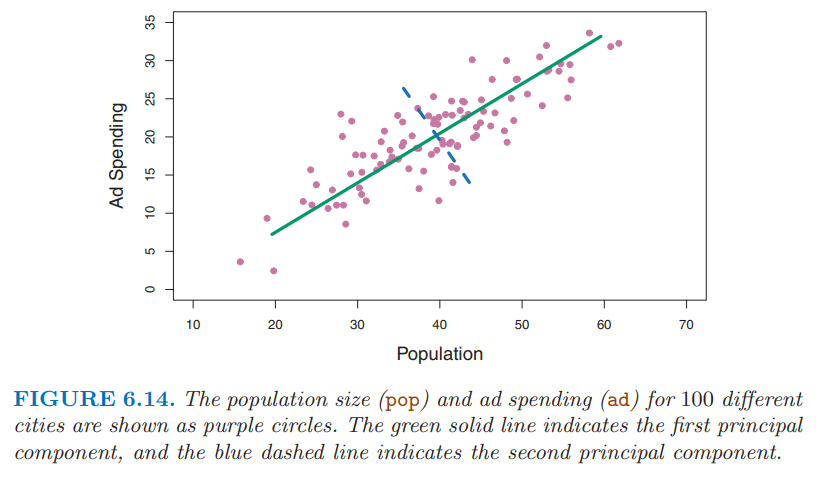
\includegraphics[scale=0.8]{images/first princ comp.png}
\end{center}
Projecting a point onto a line simply involves finding the location on the line which is closest to the point. The first principal component in the figure is given by the formula:
\begin{equation}
    Z_1 = 0.839 \times (pop - \overline{pop}) + 0.544 \times (ad - \overline{ad})
    \label{example}
\end{equation}
Here $\phi_{11} = 0.839$ and $\phi_{21} = 0.544$ are the principal component loadings, which define the direction referred to above. In \ref{example}, $\overline{pop}$ indicates the mean of all $pop$ values in this data set, and $\overline{ad}$ indicates the mean of all advertising spending. The idea is that out of every possible linear combination of $pop$ and $ad$ such that $\phi_{11}^2 + \phi_{21}^2 = 1$, this particular linear combination
yields the highest variance: i.e. this is the linear combination for which $Var(\phi_{11} \times (pop - \overline{pop}) + \phi_{21} \times (ad - \overline{ad}))$ is maximized.

\subsection{Further principal components}
After the first principal component $Z_1$ of the features has been determined, we can find the second principal component $Z_2$. The second principal component is the linear combination of $X_1,...,X_p$ that has maximal variance out of all linear combinations that are \textit{uncorrelated} with $Z_1$. The second principal component scores $z_{12}, z_{22},...,z_{n2}$ take the form
\[z_{i2} = \phi_{12} x_{i1} + \phi_{22}x_{i2} + ... + \phi_{p2} x_{ip}\]
where $\phi_2$ is the second principal component loading vector.  It turns out that constraining $Z_2$ to be uncorrelated with $Z_1$ is equivalent to constraining the direction $\phi_2$ to be orthogonal (perpendicular) to the direction $\phi_1$, and so on.\\\\
Once we have computed the principal components, we can plot them
against each other in order to produce low-dimensional views of the data. For instance, we can plot the score vector $Z_1$ against $Z_2$, $Z_1$ against $Z_3$,
$Z_2$ against $Z_3$, and so forth.\\\\
We illustrate the use of PCA on the \textbf{USArrests} data set. For each of the
50 states in the United States, the data set contains the number of arrests
per 100,000 residents for each of three crimes: \textbf{Assault}, \textbf{Murder}, and \textbf{Rape}. We also record \textbf{UrbanPop} (the percent of the population in each state living in urban areas). The principal component score vectors have length $n = 50$, and the principal component loading vectors have length $p = 4$. PCA was performed after standardizing each variable to have mean zero and standard deviation one.
\begin{center}
    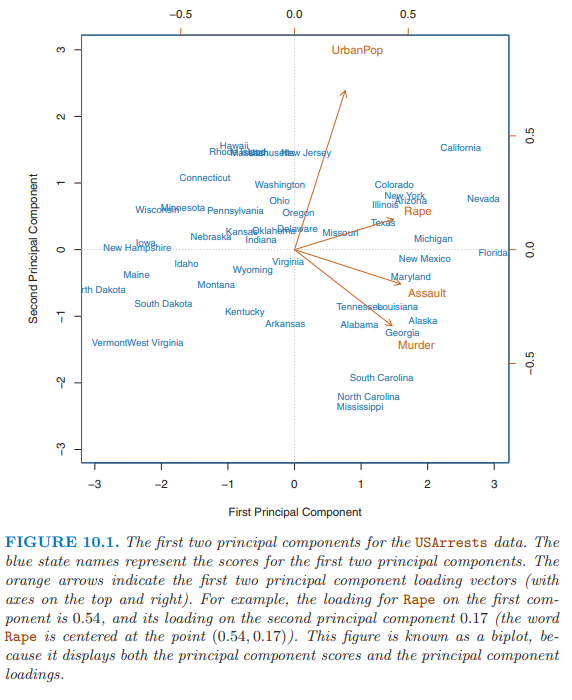
\includegraphics[]{images/biplot.png}
\end{center}
The figure above plots the first two principal components of these data. The figure represents both the principal component scores and the loading vectors in a single biplot display. The loadings are also given in the table below: 
\begin{center}
    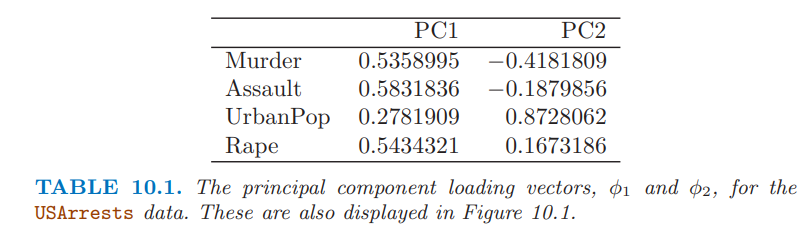
\includegraphics[scale=0.6]{images/table.png}
\end{center}
From the figure we see that the first loading vector places approximately
equal weight on \textbf{Assault}, \textbf{Murder}, and \textbf{Rape}, with much less weight on \textbf{UrbanPop}. Hence this component roughly corresponds to a measure of overall rates of serious crimes. The second loading vector places most of its weight
on \textbf{UrbanPop} and much less weight on the other three features. Hence, this
component roughly corresponds to the level of urbanization of the state. Overall, we see that the crime-related variables (\textbf{Murder}, \textbf{Assault}, and \textbf{Rape}) are located close to each other, and that the \textbf{UrbanPop} variable is far from the other three. This indicates that the crime-related variables are correlated with each other—states with high murder rates tend to have high
assault and rape rates—and that the \textbf{UrbanPop} variable is less correlated with the other three.\\\\
We can examine differences between the states via the two principal component score vectors shown in the figure. Our discussion of the loading vectors suggests that states with large positive scores on the first component, such as California, Nevada and Florida, have high crime rates, while states like North Dakota, with negative scores on the first component, have low crime rates. California also has a high score on the second component, indicating a high level of urbanization, while the opposite is true for states like Mississippi. States close to zero on both components, such as Indiana, have approximately average levels of both crime and urbanization.

\section{Another Interpretation of Principal Components}
The first two principal component loading vectors in a simulated three-dimensional data set are shown in the left-hand panel of the Figure below.
\begin{center}
    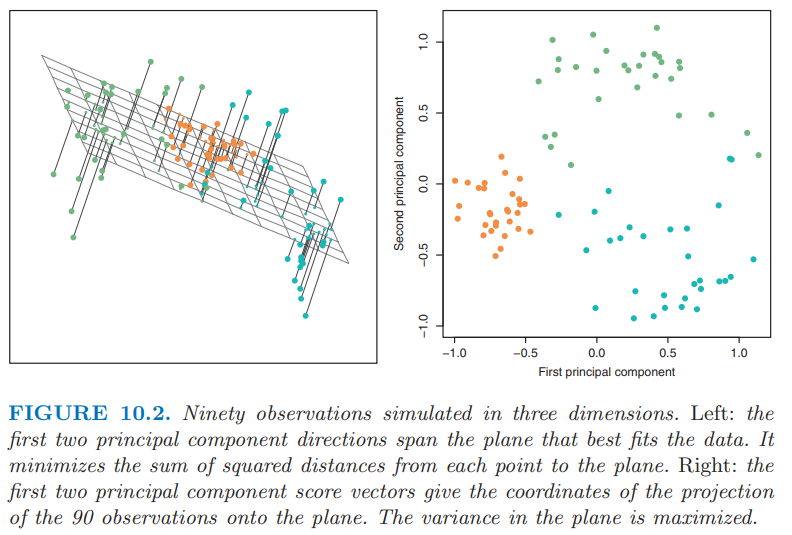
\includegraphics[scale=0.8]{images/3d pca.png}
\end{center}
Principal components provide low-dimensional linear surfaces that are closest to the observations. We expand upon that interpretation here. The first principal component loading vector has a very special property: it is the line in $p$-dimensional space that is closest to the n observations (using average squared Euclidean distance as a measure of closeness). The appeal of this interpretation is clear: we seek a single dimension of the data that lies as close as possible to all of the data points, since such a line will likely provide a good summary of the data.\\\\
The notion of principal components as the dimensions that are closest to the n observations extends beyond just the first principal component.  For instance, the first two principal components of a data set span the plane that is closest to the n observations, in terms of average squared Euclidean distance.

\section{Scaling the Variables}
We have already mentioned that before PCA is performed, the variables should be centered to have mean zero. Furthermore, the results obtained when we perform PCA will also depend on whether the variables have been individually scaled (each multiplied by a different constant).
\begin{center}
    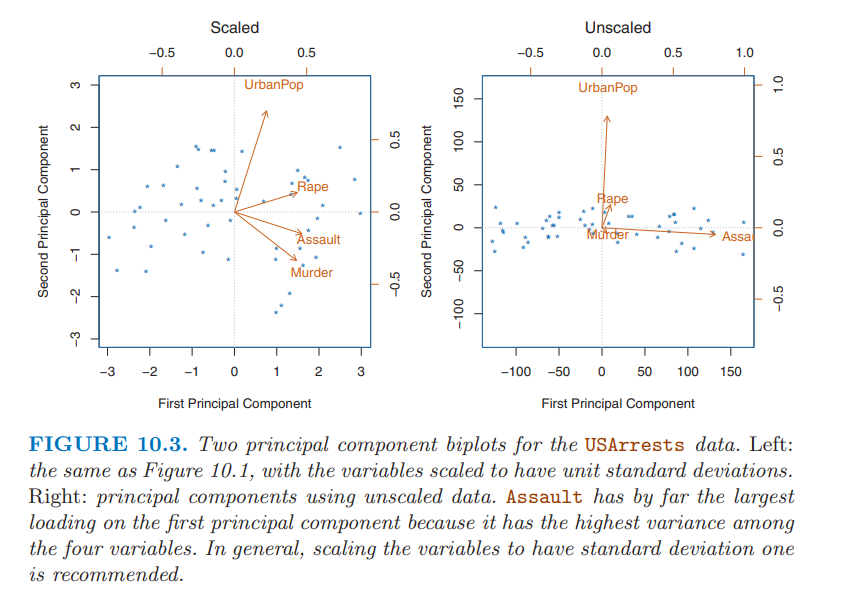
\includegraphics[scale=0.8]{images/scaled pca.png}
\end{center}
From the figure above, we see that scaling does indeed have a substantial effect on the results obtained. In these data, the variables are measured in different units; \textbf{Murder}, \textbf{Rape}, and \textbf{Assault} are reported as the number of occurrences per 100, 000 people, and \textbf{UrbanPop} is the percentage of the state’s population that lives in an urban area. These four variables have variance 18.97, 87.73, 6945.16, and 209.5, respectively. Consequently, if we perform PCA on the unscaled variables, then the first principal component loading vector will have a very large loading for \textbf{Assault}, since that variable has by far the highest variance.
\\\\
Because it is undesirable for the principal components obtained to depend on an arbitrary choice of scaling, we typically scale each variable to have standard deviation one before we perform PCA. In certain settings, however, the variables may be measured in the same units. In this case, we might not wish to scale the variables to have standard deviation one before performing PCA.

\section{The Proportion of Variance Explained}
In Figure 10.2, we performed PCA on a three-dimensional data set (lefthand panel) and projected the data onto the first two principal component loading vectors in order to obtain a two-dimensional view of the data  (i.e. the principal component score vectors; right-hand panel). We see that this two-dimensional representation of the three-dimensional data does successfully capture the major pattern in the data.\\\\
We can now ask a natural question: how much of the information in a given data set is lost by projecting the observations onto the first few principal components? That is, how much of the variance in the data is not contained in the first few principal components? More generally, we are interested in knowing the \textbf{proportion of variance explained} (PVE) by each principal component.\\\\
The total variance present in a data set (assuming that the variables have been centered to have mean zero) is defined as:
\[\sum_{j=1}^p Var(X_j) = \sum_{j=1}^p \frac{1}{n} \sum_{i=1}^n x_{ij}^2\]
and the variance explained by the $m$-th principal component is
\[\frac{1}{n}\sum_{i=1}^n z_{im}^2\]
Therefore, the PVE of the $m$-th principal component is given by:
\[\frac{\sum_{i=1}^n z_{im}^2}{\sum_{j=1}^p\sum_{i=1}^n x_{ij}^2}\]
In total, there are $min(n - 1, p)$ principal components, and their PVEs sum to one.

\section{Deciding How Many Principal Components to Use}
If we use principal components as a summary of our data, how many components are sufficient?  Unfortunately, there is no single (or simple!) answer to this question. We typically decide on the number of principal components required to visualize the data by examining a scree plot, such as the one shown in the left-hand panel of Figure 10.4.
\begin{center}
    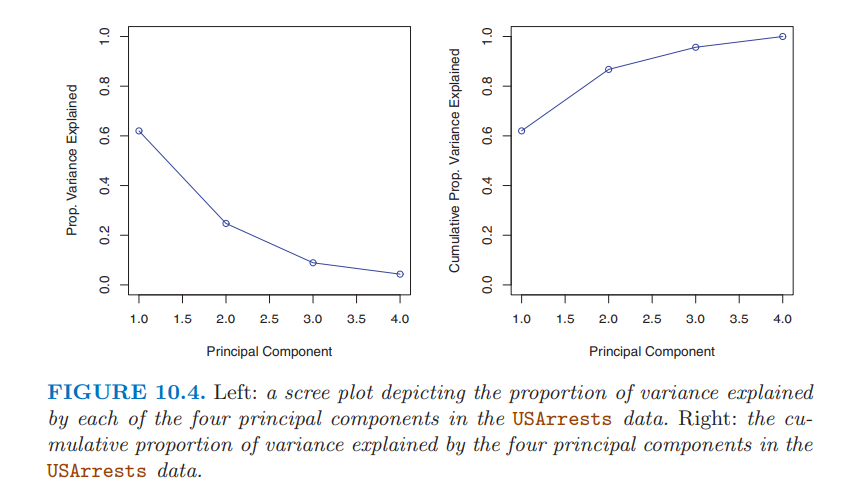
\includegraphics[scale=0.8]{images/scree plot.png}
\end{center}

\chapter{Lec 04 - PAC, Generalization and SRM}
\section{Hoeffding's Inequality}
Let's start with an example. Consider a bin full of red and green marbles.
\begin{center}
    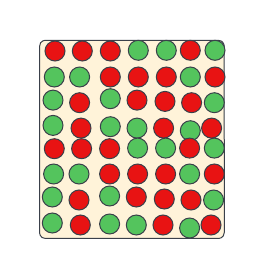
\includegraphics{images/Marbles Bin.png}
\end{center}
We denote:
\begin{itemize}
    \item $P(red) = \pi$ the probability to draw a red marble (unknown)
    \item $P(green) = 1 - \pi$ the probability to draw a green marble (unknown)
\end{itemize}
Then we draw $N$ marbles (the \textit{sample}) from the bin, \textbf{independently}\footnote{the draw of one marble doesn't influence the draw of the next one}, and we set $\sigma$ as the fraction of red marbles in the sample. So $\pi$ represent the proportion of red marbles in the \textbf{bin}, while sigma represent the proportion of red marbles in the \textbf{sample}. So the question is, does $\sigma$ say anything about $\pi$?

Consider the following formula:
\begin{center}
    \[P(|\sigma - \pi| > \epsilon) \leq 2e^{-2\epsilon^{2}N}\]
\end{center}
It's called \textbf{Hoeffding's Inequality} and it means that in a large sample (large $N$), the value of $\sigma$ is likely close to $\pi$ (within $\epsilon$).
\begin{itemize}
    \item $|\sigma - \pi| > \epsilon$ is called \textit{bad event} because when the absolute value of the difference between $\sigma$ an $\pi$ is greater than $\epsilon$, it means that $\sigma$ an $\pi$ are not so similar. This event depends on the \textit{tolerance} value $\epsilon$ that we choose.
    
    \item $2e^{-2\epsilon^{2}N}$ is a negative exponential curve.
    \begin{flushleft}
        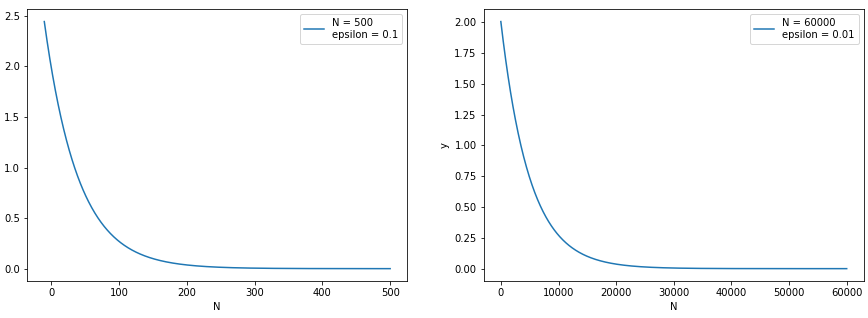
\includegraphics[scale = 0.45]{images/exp.png}
    \end{flushleft}
    As you can see from the graphs above, the curve decreases as N increases. So with larger samples, the \textit{bad event} will occur with a lower probability. Furthermore, if we set a stricter tolerance value (e.g $\epsilon$ = 0.01) the curve decreases more slowly.
\end{itemize}
For example, if we set $\epsilon$ = 0.1, $P(|\sigma - \pi| > \epsilon)$ is the probability of having a discrepancy between $\sigma$ and $\pi$ greater than 10\%; this probability, for $N$ = 200, is $\leq 0.03663127777746833$. So $\sigma = \pi$ is \textbf{P.A.C} (Probably Approximately Correct).

\section{Connection to Learning}
\begin{itemize}
    \item The target function $f: X \rightarrow Y$ is unknown
    \item The bin is the input space $X$ which contains all possible inputs for a model.
    \item The sample $N$ is the training set.
    
    \item The training set is composed by a set of pairs $\{(\textbf{x}_{1},y_{1}),...,(\textbf{x}_{n},y_{n})\}$ where $y_{i} = f(\textbf{x}_{i})$. Once we have fixed an hypothesis $h: X \rightarrow Y$ (chosen from the hypothesis space), we can "color" each example in $N$ as follows:
    \begin{itemize}
        \item green if $h(\textbf{x}) = f(\textbf{x})$
        \item red if $h(\textbf{x}) \neq f(\textbf{x})$
    \end{itemize}
    \begin{center}
        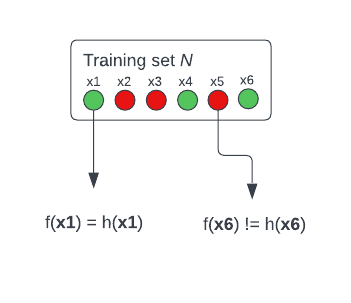
\includegraphics{images/Training set.png}
    \end{center}
\end{itemize}
Now we can say that $\sigma$ is the \textbf{empirical error}, while $\pi$ is the \textbf{ideal error} (for this $h$) and following the previous example we can observe that $\sigma$ tends to be close to $\pi$. If we have a small error $\sigma$ it's more and more probable that $h$ is a good approximation of the target function \textbf{in general} as $N$ increases. So this process \textbf{verifies} how good the approximation $h$ of $f$ is, but it has nothing to do with learning process, because $\pi$ and $\sigma$ depend on which $h$ we choose. How do we choose $h$?
\subsection{Learning}
First of all, let's change the notation:
\begin{itemize}
    \item empirical error on training data $\sigma \rightarrow E_{i}(h)$
    \item ideal error $\pi \rightarrow E_{o}(h)$
    \item $P(|E_{i}(h) - E_{o}(h)| > \epsilon) \leq 2e^{-2\epsilon^{2}N}$. The bound depends on $h$
\end{itemize}
The hypothesis space $H \equiv \{h_{1}, h_{2},...,h_{m}\}$ it's composed by many different hypotheses $h_{1},..,h_{m}$ and each of them has an empirical error $E_{i}(h_{i})$ and an ideal error $E_{o}(h_{i})$. Learning algorithms search in the hypothesis space (following some criterion) and select an hypothesis $h_{i}$ that minimizes $E_{o}(h_{i})$. However, the Hoeffding's Inequality can't be used for learning because in Supervised Learning we have to choose among several hypotheses. If we consider a worst case analysis, where all the bad events over the hypothesis space are \textbf{disjointed}, we have to bound the probability of interest in the following way:
\[P[|E_{i}(h_{i}) - E_{o}(h_{i})| > \epsilon] \leq \sum_{m=1}^{M}P[|E_{i}(h_{m}) - E_{o}(h_{m})| > \epsilon] \leq 2Me^{-2\epsilon^{2}N}\] where $M$ is the number of hypotheses (can also be infinite). \newline

The formula above says that since $h_{i}$ can be any of all $h_{1},..,h_{m}$ hypotheses in the hypothesis space, the bad event $|E_{i}(h_{i}) - E_{o}(h_{i})| > \epsilon$ can happen for $h_{1}$ \textbf{or} for $h_{2}$ \textbf{or} for $h_{3}$ \textbf{or} ... for $h_{m}$. So, since we are assuming that all bad events are disjointed ($P(A \cup B) = P(A) + P(B)$), $P[|E_{i}(h_{i}) - E_{o}(h_{i})| > \epsilon]$ must be bounded by $\sum_{m=1}^{M}P[|E_{i}(h_{m}) - E_{o}(h_{m})| > \epsilon]$. Note that for very big M the resulting bound is $>>1$, so it's useless.\newline

Just to recap a little bit:
\begin{itemize}
    \item \textbf{Testing:} Hoeffding's Inequality can help us to verify if a \textbf{fixed} hypothesis $h$ is a good approximation of the target function $f$ over a sample $N$.
    \item \textbf{Training:} Hoeffding's Inequality is not so useful for learning process since we have to choose among several hypotheses.
\end{itemize}

Fortunately, bad events are not always disjointed but they are overlapped.
\begin{center}
    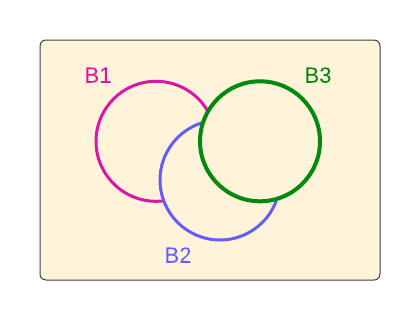
\includegraphics{images/Overlapped Sets.png}
\end{center}
So $M$ can be replaced by the \textbf{growth function} $m_{H}(N) \leq 2^{N}$ which is related to the complexity of the hypothesis space. When the hypothesis space has a low complexity bad events overlap a lot ($m_{H}(N) << 2^{N}$), when it's very complex they tend to be disjointed. So if $m_{H}(N)$ is \textbf{polynomial} with respect to $N$, the upper bound $2Me^{-2\epsilon^{2}N}$ tends to 0 as $N$ increases. How can i compute the complexity of the hypothesis space ?
\subsection{VC-Dimension}
\begin{center}
    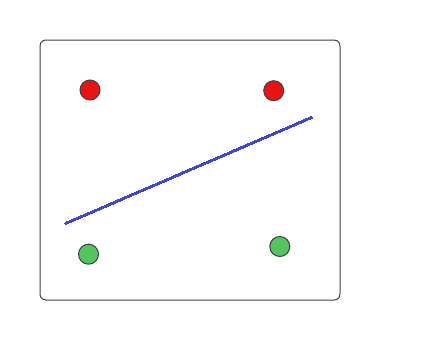
\includegraphics{images/Dichotomy 1.png}
    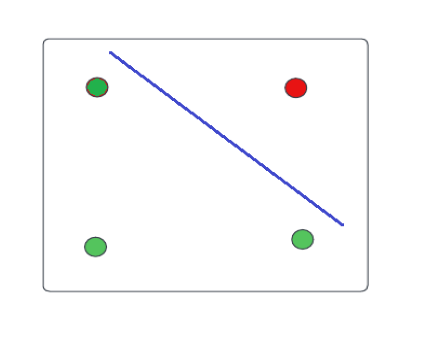
\includegraphics{images/Dichotomy 2.png}
\end{center}
Let's consider a plane with 4 points. If we choose the hyperplanes in $\mathbb{R}^{2}$ as hypothesis space $H$ we can divide the points with a line and classify them with two colors (red and green). These partitions are called dichotomies. Note that this particular $H$ \textbf{can't} implement all possible dichotomies.
\begin{figure}[h]
    \centering
    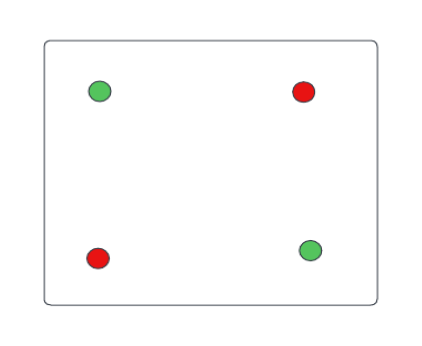
\includegraphics{images/Dichotomy 3.png}
    \caption{This classification can't be implemented by any hyperplane in $H$}
\end{figure} \newline
\begin{itemize}
    \item \textbf{Shattering: } Given $S \subset X, S$ is shattered by the hypothesis space $H$ iff 
    \[\forall S^{'} \subseteq S, \exists h \in H, s.t. \forall x \in S, h(x) = 1 \iff x \in S^{'}\]
    That means that $H$ is able to implement all possible dichotomies of $S$.
    
    \item \textbf{VC-dimension: } The VC-dimension of an hypothesis space $H$ defined over an instance space $X$ is the size of the largest finite subset of $X$ shattered by $H$: 
    \[VC(H) = \max_{S \subseteq X}|S|\]
    such that S is shattered by $H$.
\end{itemize}

If we consider $H_{1} = \{f_{w,b}(y) | f_{w,b}(y) = sign(w \cdot y + b), w \in \mathbb{R}^{2}, b \in \mathbb{R}\}$ as hypothesis space (hyperplanes in $\mathbb{R}^{2}$), as we saw before $VC(H_{1}) = 3$ because it doesn't exist \textbf{any} configuration of 4 points that can be shattered by $H_{1}$. In general, VC-dimension of hyperplanes in $\mathbb{R}^{n} = n + 1$: in 2 dimensions $VC(H) = 3$, in 3 dimensions $VC(H) = 4$ and so on.

\subsection{VC bound and SRM}
Consider a binary classification learning problem with:
\begin{itemize}
    \item Training set $S = \{(\textbf{x}_{1},y_{1}),...,(\textbf{x}_{n},y_{n})\}$.
    \item Hypothesis space $H = \{h_{\theta}(\textbf{x})\}$.
    \item Learning algorithm $L$, returning the hypothesis $g = h_{\theta}^{*}$ minimizing the empirical error on $S$, that is $g = argmin_{h \in H}error_{S}(h)$.
\end{itemize}
It is possible to derive \footnote{We will not see the derivation here.} an upper bound of the ideal error which is valid with probability $(1-\delta)$, $\delta$ being arbitrarily small, of the form:
\[error(g) \leq error_{S}(g) + F(\frac{VC(H)}{n},\sigma)\]
where $error(g)$ is the ideal error. The term $F(\frac{VC(H)}{n},\sigma)$ is called \textbf{VC-confidence} and it depends on:
\begin{itemize}
    \item The training size $n$ (inversely).
    \item The VC-dimension of $H VC(H)$ (proportionally).
    \item The confidence $\sigma$ (inversely).
\end{itemize}
As the VC-dimension grows, you usually observe that the empirical error decreases and that the VC confidence increases. So you can use the inductive principle \textbf{Structural Risk Minimization (SRM)} in order to minimize the right side of the confidence bound to get a tradeoff between the empirical error and the VC confidence.
\begin{figure}[h]
    \centering
    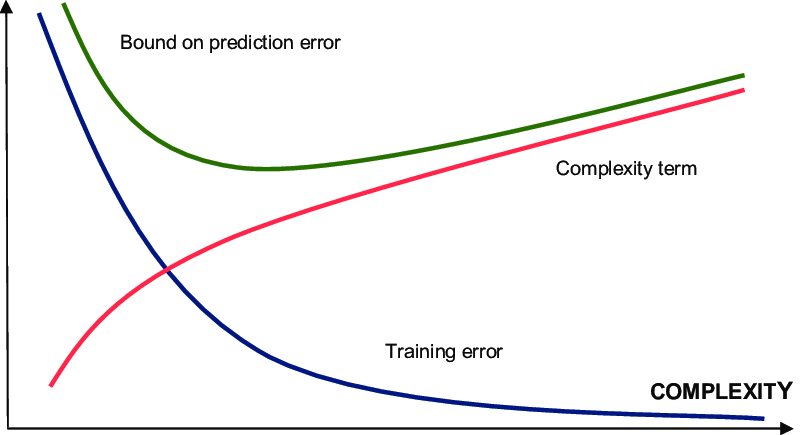
\includegraphics[scale=0.3]{images/Structural-risk-minimization-principle-Vapnik-1998.png}
    \caption{The green curve \textit{Bound on prediction error} is the sum between empirical error curve and VC confidence curve.}
\end{figure}

\chapter{Lec 05 - Decision Trees I}

\section{Decision Trees}
Decision trees (DTs) allow to learn \textbf{discrete} functions that are representable by a tree. Given a training set instance like the following one:
\begin{center}
    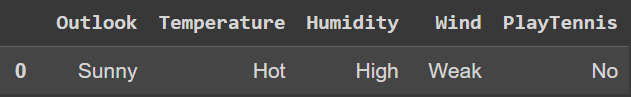
\includegraphics[scale=0.7]{images/Dataset instance.png}
\end{center}
\textbf{Attributes} are [$Outlook, Temperature, Humidity, Wind$], while $PlayTennis$ is the feature to predict (we want to predict if a day is suitable to play tennis). The values that $PlayTennis$ can take are called \textbf{classes}.
In a decision Tree:
\begin{itemize}
    \item An \textbf{inner node} corresponds to an attribute of an instance.
    \item A \textbf{branch} descending from a node corresponds to one of the possible values the attribute can assume.
    \item A \textbf{Leaf node} assigns a classification.
\end{itemize}
The classification of an instance works in the following way:
\begin{itemize}
    \item Start from the root
    \item Select the attribute attached to the current node
    \item Select a subtree following the branch corresponding to the value of that attribute in the instance.
    \item If we reach a leaf node we classify the instance with the associated label, else return to step 2.
\end{itemize}
Let's consider the following Decision Tree related to the \textit{tennis dataset} mentioned before.
\begin{center}
    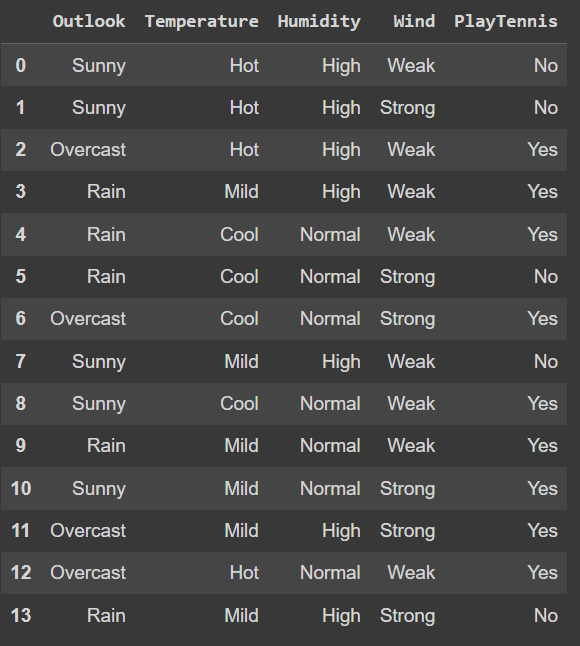
\includegraphics[scale=0.5]{images/layTennisDataset.png}
    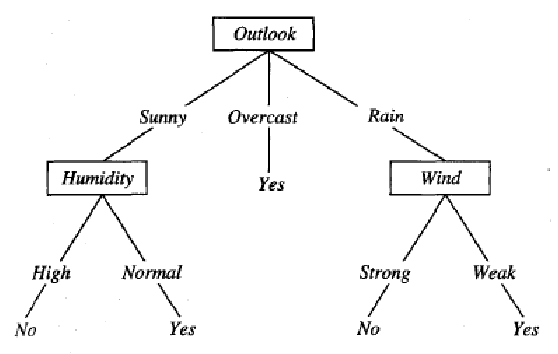
\includegraphics[scale=0.45]{images/decision tree playtennis.png}
\end{center}
The instance [O=Sunny, T=Hot, H=High, W=Strong] is classified with label \textit{NO} (not suitable to play tennis). In fact, following the path $O=Sunny \rightarrow H=High$ we end up in a leaf node with label 'NO'. Note that a decision tree can be represented as a boolean function:
\begin{itemize}
    \item Each path from the root to a leaf node codifies a conjunction of constraints on the attribute values of the instance.
    \item Different paths that lead to a same classification codify disjunctions of conjunctions.
\end{itemize}
So the classification can be seen as a series of \textbf{DNF} (disjunctive normal form) formulas, one DNF for each class. For example, DNF corresponding to \textit{YES} is (O=Sunny \textbf{and} H=Normal) \textbf{or} (O=Overcast) \textbf{or} (O=Rain \textbf{and} W=Week). This last feature, absent in most of the machine learning techniques, makes decision trees comprehensible and interpretable by humans. So they are particularly interesting for medical, biological and financial applications where interpreting a model is very important.
\subsection{DTs learning algorithm}
A recursive implementation of the \textbf{ID3} algorithm (the most popular learning algorithm for DTs) is the following:\newline
\textbf{ID3($S$, $A$)} Given a sample $S$ and a set of attributes $A$
\begin{itemize}
    \item If examples in $S$ are all of the same class $c$, return a leaf node with label $c$.
    \item if $A$ is empty, return a leaf node with label equals to the majority class\footnote{the class associated with the largest number of examples in $S$} in $S$.
    \item Select $a \in A$, the \textbf{optimal} attribute in $A$ and remove it from $A$ $(A = A - a)$.
    \item For each distinct value $v_{j}$ that $a$ can take in $S_{a}$, partition $S$ according to $v_{j}$ ($S_{a=v_{j}}$) and return the tree T having sub-trees the trees obtained by recursively calling \textbf{ID3}($S_{a=v_{j}}, A$).
\end{itemize}
Note that in the $4^{th}$ point of the algorithm, when you partition $S$ according to $v_{j}$, it is possible that in $S$ there are instances having only some of the possible values that the best attribute $a$ can take, so you have to consider only these values in that specific $S_{a}$ partition.

\subsection{Select optimal attribute}
Different learning algorithms for DTs mainly differ in how they select the optimal attributes. ID3 uses the concepts of \textbf{Entropy} and \textbf{Information Gain}.
\begin{itemize}
    \item \textbf{Entropy}: Let $C$ be the number of classes and $S_{c}$ the subset of $S$ of instances of class $c$, the entropy is computed as follows:
    \[E(S) = -\sum_{c=1}^{C}p_{c}log_{2}(p_{c})\]
    where $p_{c} = \frac{|S_{c}|}{|S|}$.
    In the case of binary classification (only two classes), it has the following shape:
    \begin{center}
        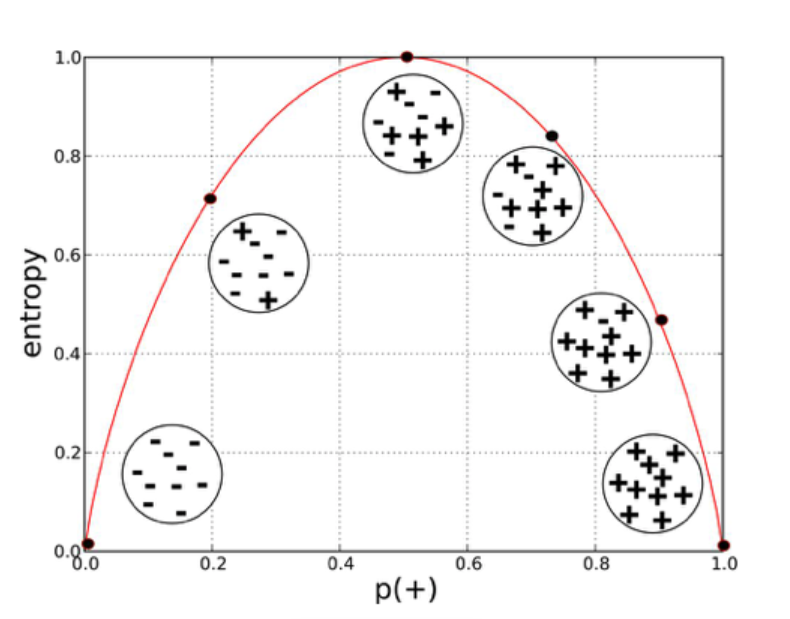
\includegraphics[scale=0.5]{images/entropy.png}
    \end{center}
    Entropy is lowest at the extremes, when $S$ either contains no positive instances or only positive instances (sample is pure without disorder) and it's highest where positive and negative instances are evenly split.
    
    \item \textbf{Information Gain:} The optimal attribute will be the one that maximizes the Information Gain $G(S,a)$
    \[G(S,a) = E(S) - \sum_{v \in V(a)}\frac{|S_{a=v}|}{|S|}E(S_{a=v})\]
    where 
    \begin{itemize}
        \item $S$ is the sample (could be the entire training set or a partition of it depending on which level of recursion we are in: see $4^{th}$ point of the ID3 algorithm.
        \item $a$ is the selected attribute.
        \item $E(S)$ is the total entropy of $S$.
        \item $V(a)$ is the set of distinct values that $a$ can take in $S_{a}$.
        \item $S_{a=v}$ is the partition of $S$ in which instances have the attribute $a$ equals to $v$.
    \end{itemize}
\end{itemize}
We can generalize the notion of Information Gain to other impurity measures:
\begin{itemize}
    \item \textbf{Cross-Entropy:} $I_{H} = -\sum_{c=1}^{C}p_{c}log_{2}(p_{c})$.
    \item \textbf{Gini Index:} $I_{G} = 1 - \sum_{c=1}^{C}(p_{c}^{2})$.
    \item \textbf{Misclassification:} $I_{E} = 1 - \max_{c}(p_{c})$.
\end{itemize}
Let $I$ be any of the impurity criteria mentioned above, the Information Gain definition becomes:
\[G(S,a) = I(S) - \sum_{v \in V(a)}\frac{|S_{a=v}|}{|S|}I(S_{a=v})\]
\subsection{DTs problems}
The information gain tends to favor attributes that can assume many possible values. \newline
\textbf{Example:} Consider a sample $S$ with an attribute consisting in dates. This attribute is likely going to be the one with maximum gain because each subset $S_{a=v}$, that is composed by \textbf{only one instance}, will be pure with zero impurity. In fact, the entropy of a subset with only one class is 0. \newline \newline
Another problem is the overfitting: The model is very accurate on training data but not on test data. 
\begin{center}
    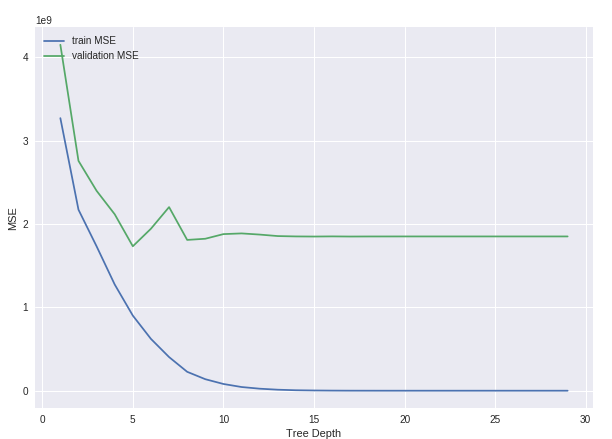
\includegraphics[scale=0.4]{images/overfitting dts.png}
\end{center}
We can observe that the problem increases as the number of nodes increases. A partial solution can be to set a minimal number of examples to accept on leaf nodes or limit the maximal depth of the tree (at a certain point i don't split $S$ anymore and i consider that node as a leaf with label the majority class in $S$).
\subsection{When to use DTs}
Decision trees are useful when dealing with problems having the following characteristics:
\begin{itemize}
    \item A fixed set of attributes and, for each attribute, a fixed set of values
    \item Discrete values for the attributes (decision trees can also be extended to deal with continuous values).
    \item Target function with discrete output values (classification problems).
    \item The target function can be approximated by disjunctions of boolean functions (Inductive bias).
    \item Training examples can contain noise (two or more instances with same attributes values but different classes) and missing values.
    
\end{itemize}
%You can find my implementation from scratch of ID3 algorithm on my GitHub(\url{https://github.com/riccardocappi/Machine_Learning_Course/blob/main/Decision_Trees_Python.ipynb}), Colab notebook(\url{https://colab.research.google.com/drive/1K2sytaFCfyT-FVMHNb7jvOi7bben_cah?usp=sharing}) or uploaded on the forum of ML course(\url{https://stem.elearning.unipd.it/mod/forum/discuss.php?d=2484}).

\chapter{Lec 06 - Probability}

\section{Probability - terminology}
\begin{itemize}
    \item \textbf{Random variable:} a variable that can take different values randomly

    \item \textbf{Probability distribution:} a description of how likely a random variable x (or a set of random variables) is to take each of its possible states.\newline\newline
    \textbf{Discrete variables:} Probability distribution is described by a \textbf{Probability mass function}
    \begin{itemize}
        \item The domain of $P$ is the set of all possible states of x ($k$ different values).
        
        \item $\forall \, x \in \text{x} \, 0 \leq P(\text{x} = x) \leq 1$
        
        \item $\sum_{x \in \text{x}}P(x) = 1$
    \end{itemize}
    E.g. Uniform distribution $\forall \, x \in \text{x} \, P(\text{x} = x) = \frac{1}{k}$\newline\newline
    \textbf{Continuous variables:} Probability distribution is described by a \textbf{Probability Density Function} (PDF) 
    \begin{itemize}
        \item The domain of $p$ is the set of all possible states of x

        \item $\forall \, x \in \text{x}\, p(x) \geq 0$

        \item $\int p(x) dx = 1$
    \end{itemize}
    E.g. Gaussian distribution

    \item \textbf{Joint probability distribution:} Probability distribution over 2 or more variables $P(\text{x} = x, \text{y} = y)$

    \item \textbf{Gaussian distribution}: The one-dimensional Gaussian with mean $\mu$ and standard deviation $\sigma$ has the following shape:
    \[G(x) = \frac{1}{\sigma \sqrt{2\pi}}e^{-\frac{(x-\mu)^{2}}{2\sigma^{2}}}\]
    \begin{center}
        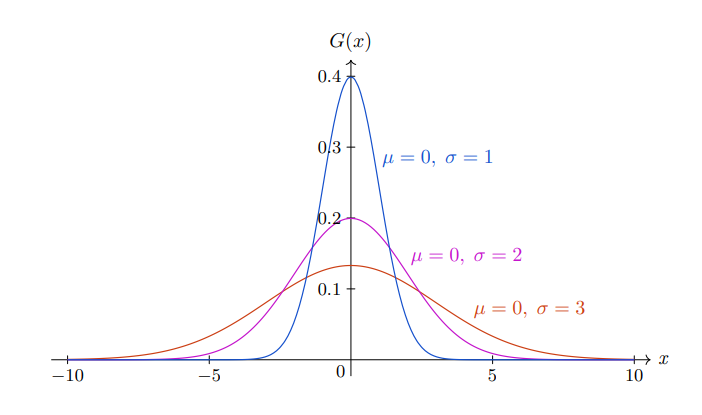
\includegraphics[]{images/Gaussian.png}
    \end{center}

    \item \textbf{Shannon Entropy (discrete variable):} 
    We can apply information theory to calculate the amount of information there is in an event. This is called \textit{self-information} and can be calculated for a \textbf{discrete} event $x$ as follows:
    \[I(x) = -log\,(P(x))\]
    where $log()$ is the base-2 logarithm and $P(x)$ is the probability of the event $x$ \footnote{other bases can be used, $e$ for example}.
    \newline\newline
    The choice of the base-2 logarithm means that the units of the information measure is in bits (binary digits). This can be directly interpreted as the number of bits required to represent an event. If the probability that an event occurs is $0.5$, we need 2 bits two represent it ($0$ fail, $1$ success); if the event occurs with probability $0.125$, we need $3$ bits to represent it (remember $y = log_a\,(x) \iff x = a^y$).
    \newline\newline
    The Shannon entropy of a \textbf{distribution} is the \textbf{expected} amount of information in an event drawn from that distribution:
    \[H(\text{x}) = - E_{x \sim P(\text{x})}[log(P(x))] = -\sum_i P(x_i) log\,P(x_i)\]
    It provides a lower bound on the number of bits needed \textbf{on average} to encode a symbol drawn from the distribution.\newline\newline
    Distributions that are nearly deterministic (where the outcome is nearly certain) have low entropy; distributions that are closer to uniform have high entropy.
    

    \item \textbf{Kullback-Leibler divergence and Cross Entropy:} Let's consider two probability distributions $P(x)$ and $Q(x)$. How can we measure how different they are?
    \begin{itemize}
        \item Kullback-Leiber divergence:
        \[D_{KL}(P \,||\, Q) = E_{x \sim P}\left[ log\frac{P(x)}{Q(x)} \right] = E_{x \sim P}[ log\, P(x) - log\, Q(x)] = \sum_i P(x_i) log\, \left(\frac{P(x_i)}{Q(x_i)}\right)\]
        It is not a true distance because it is not symmetric:
        \[D_{KL}(P \, ||\, Q) \neq D_{KL}(Q \, ||\, P)\]
        It is the measure of information lost when $Q$ is used to approximate $P$.


        \item Cross Entropy:
        \[H(P, Q) = H(P) + D_{KL}(P\, ||\, Q) = -E_{x \sim P}[log\, Q(x)]\]
        where $H(P)$ is the entropy of $P$. Note that minimizing the Cross Entropy of $P$ with respect to $Q$ is equivalent to minimize KL divergence between $P$ and $Q$. (if $P$ is given, $H(P)$ and $E_{x \sim P}[log\, P(x)]$ are constants). If $P$ is a fixed distribution minimize KL divergence or minimize CE is the same, but CE is easier to compute.
    \end{itemize}

    \item \textbf{Maximum likelihood estimation:} Is a principled way to derive estimators (models). Consider $n$ examples $Tr = \{\textbf{x}^{1}, ..., \textbf{x}^{n}\}$ drawn i.i.d. from $p_{data}$ (which is not known in advance). With machine learning we want to estimate this probability $p_{data}$ with some models that depend on a set of parameters $\theta$.\newline\newline
    Let's consider a family of parametric probability distributions (models) $p_{model}(\textbf{x}; \theta)$. It maps a point $\textbf{x}$ to a real number, estimating $p_{data} (\textbf{x})$. How can we find $\theta$ in such a way that $p_{model}$ and $p_{data}$ are as close as possible ? A possible formalization of this problem is given by the Maximum Likelihood estimation for $\theta$:
    \[\theta_{ML} = argmax_{\theta}\, p_{model}(Tr; \theta) = argmax_{\theta}\prod_{i = 1}^{n}p_{model}(\textbf{x}^{i}; \theta)\]
    Basically, we choose the probability distribution which is most likely to have produced our data. Note that we are assuming that all the examples are \textbf{independent} each other ($P(x, y) = P(x)P(y)$).
\end{itemize}

\section{Maximum likelihood}
Maximum likelihood (ML) is a special case of \textbf{maximum a posteriori estimation (MAP)}.
\[h_{MAP} = argmax_{h \in H}P(h|D)\]
\[= argmax_{h \in H}\frac{P(D|h)P(h)}{P(D)}\]
where:
\begin{itemize}
    \item $P(h):$ a priori probability of the hypothesis $h$
    \item $P(D):$ a priori probability of training data. It is the probability to observe exactly this training set when we don't know anything about the hypothesis.
    \item $P(h|D):$ probability of $h$ given $D$. It is the probability that $h$ is the hypothesis that generates data $D$.
    \item $P(D|h):$ probability if $D$ given $h$. Given a hypothesis $h$, it is the probability of data $D$ to be generated by $h$.
\end{itemize}
Since $P(D)$ does not depend on $h$, we can consider it as a constant and remove it from the equation.
\[= argmax_{h \in H}P(D|h)P(h)\]
If we assume uniform probabilities on the hypotheses, that is $P(h_{i}) = P(h_{j})$, we can choose the so called \textbf{maximum likelihood hypothesis} $h_{ML}:$
\[h_{ML} = argmax_{h \in H}P(D|h)\]
MAP and maximum likelihood approach make predictions using a single point estimate of $\theta$. The Bayesian approach is to make predictions using a full probability distribution over $\theta$. For example, given a new instance $\textbf{x}$, which is the most likely \textbf{classification}? The classification given by the most likely hypothesis $h_{MAP}$ is not necessarily the most likely classification. For example, given the following three possible hypothesis:
 \[P(h_{1} | D) = 0.4 \quad P(h_{2} | D) = 0.3 \quad P(h_{3} | D) = 0.3\]
 We want to classify a new instance $\textbf{x}$:
 \[h_{1}(\textbf{x}) = + \quad h_{2}(\textbf{x}) = - \quad h_{1}(\textbf{x}) = -\]
 The most likely hypothesis $h_{1}$ classifies $\textbf{x}$ with the label (+), but the most likely classification is (-). This is because the optimal (Bayes) classification of a certain instance is the class $v_{j} \in V$ which maximizes the following probability:
 \[argmax_{v_{j} \in V} = \sum_{h_{i} \in H}P(v_{j} | h_{i})P(h_{i} | D)\]
 where $V$ is the set of possible labels.\newline\newline
 However, in real-world problems having the probabilities $P(h_{i} | D)$ is almost impossible. Therefore, we usually make the assumption of considering the classification made by $h_{map}$ as most probable.

 \subsection{Maximum likelihood estimation}
 As we said before, the maximum likelihood estimation is defined as follows:
 \[\theta_{ML} = argmax_{\theta}\, p_{model}(Tr; \theta) = argmax_{\theta}\prod_{i = 1}^{n}p_{model}(\textbf{x}^{i}; \theta)\]
 However, computing the product of many probability is unstable. Therefore, we can apply the $log$ and the $argmax$ does not change (log-likelihood).
 \[\theta_{ML} = log(argmax_{\theta}\prod_{i=1}^{n}p_{model}(\textbf{x}^{(i)}; \theta))\]
 \[= argmax_{\theta}\sum_{i = 1}^{n}log\, p_{model}(\textbf{x}^{(i)}, \theta)\]
 We can equivalently divide by $n$ to express maximum likelihood as an expectation over training data:
 \[\theta_{ML} = argmax_{\theta}E_{x \sim \hat{p}_{data}}[log \, p_{model}(x; \theta)]\]
where $\hat{p}_{data}$ is an empirical discrete distribution that we get over the examples in the training set. This implies that maximum likelihood minimizes the dissimilarity between $\hat{p}_{data}$ and $p_{model}$, measured by the KL divergence. It also corresponds to minimize the \textbf{cross-entropy} between the two distributions.

\subsection{Conditional log likelihood}
We can use maximum likelihood to estimate a \textbf{conditional} probability $P(\textbf{y} | \textbf{x}; \theta)$ to predict $\textbf{y}$ given $\textbf{x}$ (supervised learning).
\[\theta_{ML} = argmax_{\theta} P(\textbf{Y} | \textbf{X}; \theta)\]
If input examples are i.i.d.
\[\theta_{ML} = argmax_{\theta}\sum_{i=1}^{n}log\, P(\textbf{y}^{(i)} | \textbf{x}^{(i)}; \theta)\]
Consider any real-valued target function $f$ and learning examples $\langle 
 \textbf{x}_{i}, d_{i}\rangle$ where $d_{i}$ has some noise:
 \begin{itemize}
     \item $d_{i} = f(\textbf{x}_{i}) + e_{i}$
     \item $e_{i}$ is a random variable (noise) extracted independently, for each $\textbf{x}_{i}$, according to a Gaussian distribution with mean 0.
 \end{itemize}
 It can be shown that the maximum likelihood hypothesis is the one that minimizes the mean squared error:
 \[\theta_{ML} = argmin_{\theta} \sum_{i=0}^{m}(d_{i} - \hat{y}_{i})^{2}\]
maximizing the log-likelihood with respect to $\theta$ yields the same estimate of the parameters $\theta$ as does minimizing the mean squared error.

\chapter{Lec 07 - Neural Networks I}

\section{Neural Networks}
An artificial neuron is a unit that computes a non-linear function over the inputs. Its output depends on the input and on the set of \textbf{weights}. These weights have to be learned.\newline\newline
An \textbf{Artificial Neural Network} is a system consisting of interconnected units that compute nonlinear (numerical) functions. Adjustable weights are associated with connections among units.\newline\newline
Deep Feed Forward Neural Networks, also called multi-layer perceptrons (MLP), approximate a function $f^{*}$ that maps an input $x$ to a category $y$. The MLP defines a mapping $\hat{y} = f(x;\theta)$ where $\theta$ is the set of parameters. They are typically represented as a composition of many different functions $f(x) = f^{(3)}(f^{(2)}(f^{(1)}(x)))$. The intermediate layers are called \textbf{hidden layers}, while the final layer is called \textbf{output layer}.\newline\newline
Multiple layers of cascaded units makes a Neural Network able to implement complex non linear functions. The non linearity of the model is given by the activation functions. In fact, without them (linear activation) the result of the model, even if it’s very complex, would still be linear.\newline\newline
\textbf{Example:}\newline
Let's try to define a linear model that predicts the XOR function.
\[Tr = \{ ([0,0], 0), ([0, 1], 1), ([1,0],1), ([1,1], 0)\} \quad f(\textbf{x};\textbf{w};b) = \textbf{x}\textbf{w}^{T} + b\]
The XOR function \textbf{cannot} be learned by any linear classifier. In order to solve this problem, we can define a two-layers Neural Network with the addition of the ReLU activation function $ReLU(y) = max(0, y)$. The networks becomes:
\[f(\textbf{x}; \textbf{W}, \textbf{c}, \textbf{w}, b) = \textbf{w}^{T} \, max(0, \textbf{W}\textbf{x}^{T} + \textbf{c}) + b\]
the following parameters values provide a solution to the XOR problem:
\[
    \textbf{W} =
    \begin{bmatrix}
        1 & 1\\
        1 & 1
    \end{bmatrix},
    \,\,
    \textbf{c} = 
    \begin{bmatrix}
        0 \\
        -1
    \end{bmatrix},
    \,\,
    \textbf{w} = 
    \begin{bmatrix}
        1 \\
        -2
    \end{bmatrix},
    \,\,
    b = 0
\]
Note that the first hidden layer has two nodes.\newline\newline
The most common activation functions are the following:
\begin{center}
    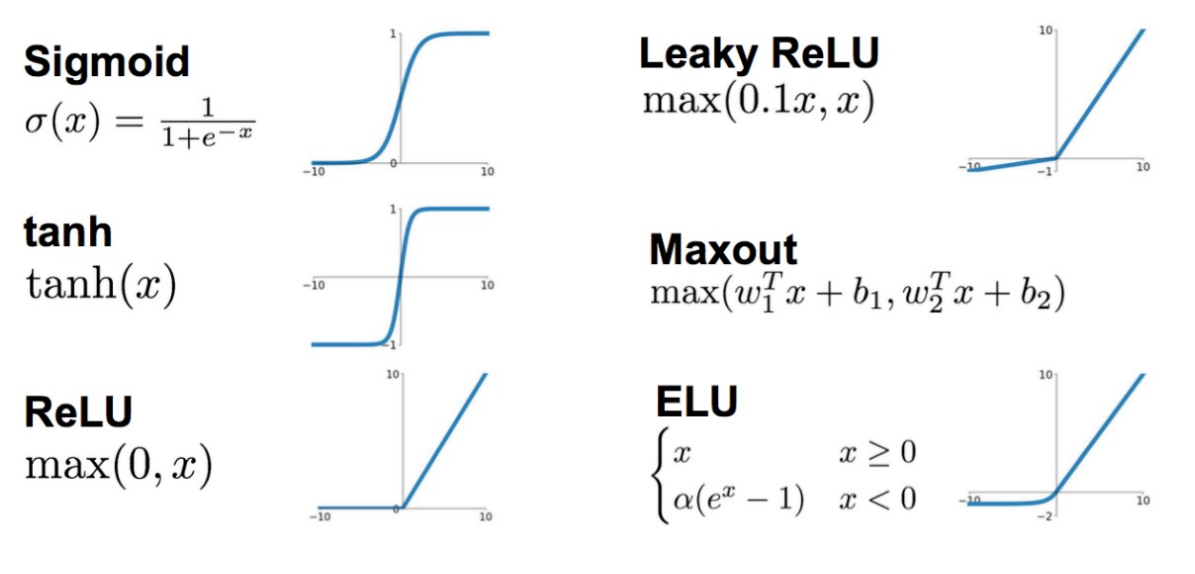
\includegraphics[scale = 0.6]{images/Activation Functions.png}
\end{center}
In general, the goal is to have a more complex decision surface. We can achieve this goal by using non-linear activation functions and stacking several hidden layers. In the XOR example above, the initial points are mapped by the first hidden layer into a new space where they are linearly separable. Thanks to this, the output linear layer is able to classify the points correctly.

\section{Learning in a Neural Network}
In general, the problem of how to update the weights of a model in order to minimize the committed error is called \textbf{credit assignment problem}. A possible solution is to make a single neuron \textbf{derivable} and exploit gradient descent technique to learn the \textit{right} weights. In order to make a neuron derivable, its activation function must be derivable.\newline\newline
Linear models (e.g. SVM) are formulated as \textbf{convex models}. However, the non-linearity in neural networks makes the problem \textbf{non-convex}. It means that there is no guarantee of achieving the global optimum. Furthermore, the way in which the weight of a NN are initialized has a strong impact on the solution that the model will find.

\section{Cost Function}
A important aspect of the design of a deep neural network is the choice of the cost function. In most cases, the model defines a distribution $p(\textbf{y} | \textbf{x}; \theta)$ and the cost function is the cross-entropy between training labels and network predictions (negative log-likelihood):
\[J(\theta) = - E_{(x,y) \sim \hat{p}_{data}}log\, p_{model}(\textbf{y}|\textbf{x})\]
The specific form of the cost function changes from model to model. The output representation $\textbf{h} = f(\textbf{x};\theta)$ determines the form of the cross-entropy function.
\begin{itemize}
    \item \textbf{Linear Regression:} If we assume that the target values are distributed according to a Gaussian distribution $G$, we can think our output layer as to produce the mean of $G$.
    \[\hat{\textbf{y}} = \textbf{W}^{T}\textbf{h} + \textbf{b}\]
    \[G(\textbf{y};\hat{\textbf{y}}; \textbf{I})\]
    As we already seen, in this case maximizing the likelihood corresponds to minimize the mean squared error.
    \[J(\theta) = \frac{1}{2}E_{p \sim \hat{p}_{data}}(y - f(\textbf{x}; \theta))^{2} + constant\]
    Basically, this is a motivation of why the mean squared error cost function is suitable for linear regression.

    \item \textbf{Binary classification:} In this case we assume that our targets are distributed according to a Bernoulli distribution. This distribution depends on a single parameter $\phi \in [0, 1]$:
    \begin{itemize}
        \item $P(\text{x} = 1) = \phi$
        \item $P(\text{x} = 0) = 1 - \phi$
    \end{itemize}
    In general:
    \[P(\text{x} = x) = \phi^{x}(1 - \phi)^{1-x}\]
    The NN just needs to predict $P(\text{y} = 1 | \textbf{x})$. Therefore, we want to force this number to lie in $[0, 1]$. For example, we can use the following function:
    \[P(\text{y} = 1|\textbf{x}) = max(0, min(1, \textbf{w}^{T}\textbf{h} + b))\]
    However, this is not a good choice for gradient descent. In fact, if the output is outside $[0, 1]$ the function is not derivable and the gradient will always be 0. We want to ensure that there is always some gradient when the model is wrong. An alternative way to force the output to lie in $[0, 1]$ is to use an \textbf{output} linear layer with a \textbf{sigmoid activation function}.
    \[\hat{y} = \sigma(\textbf{w}^{T}\textbf{h} + b)\]
    where $\sigma$ is a Sigmoid or Logistic function:
    \[\sigma(x) = \frac{1}{1 + e^{-x}}\]
    \begin{center}
        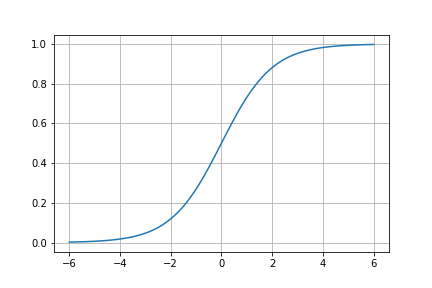
\includegraphics[scale = 0.5]{images/sigmoid.png}
    \end{center}
    An output unit is composed of two components:
    \begin{itemize}
        \item $z = \textbf{w}^{T}\textbf{h} + b$
        \item $\sigma(\cdot)$: the activation function to \textbf{convert $z$ into a probability} (in order to apply maximum likelihood optimization).
    \end{itemize}
    How can we define a probability distribution over $y$ using the value $z$ ? The sigmoid can be motivated by constructing an unnormalized probability distribution $\hat{P}(y)$, which does not sum to 1. We assume that the unnormalized probabilities are linear in $y$ and $z$.
    \[log\, \hat{P}(y) = yz \quad i.e. \,\, log\, \hat{P}(y = 1) = z, \,\, log\, \hat{P}(y = 0) = 0\]
    We can exponentiate to obtain the unnormalized probabilities:
    \[\hat{P}(y) = e^{yz}\]
    Then, we normalize to obtain a proper probablity:
    \[P(y) = \frac{e^{yz}}{\sum_{y'=0}^{1} e^{y'z}} = \sigma((2y - 1)z)\]
    where:
    \begin{itemize}
        \item $P(y = 1) = \frac{1}{1 + e^{-z}}$
        \item $P(y = 0) = \frac{1}{1 + e^{z}}$
    \end{itemize}
    As we already seen, the cost function used with maximum likelihood is the negative-log likelihood. Therefore, the loss function for maximum likelihood learning of a Bernoulli parametrized by a sigmoid is:
    \[J(\theta) = -log\, P(y|\textbf{x}) = -log\,\sigma((2y - 1)z) = \zeta((1 - 2y)z)\]
    where $\zeta(x) = log(1 - exp(x))$ is called \textbf{softplus} function.\newline\newline
    This approach to predicting the probabilities in log-space is natural to use with maximum likelihood learning. The log in the cost function undoes the exp of the sigmoid. Without this effect, the saturation of the sigmoid could prevent gradient- based learning from making good progress.\newline\newline
    The saturation (i.e. when the gradient is very small) occurs when $y = 1$ and $z$ is very positive or $y = 0$ and $z$ is very negative, that is, when the model has the right answer.\newline\newline
    With other cost functions, such as MSE, we'll be able to find a solution but it would \textbf{not} be the maximum-likelihood solution.

    \item \textbf{Multi-class classification:} In this case the output has to be a probability distribution over a discrete variable with $n$ possible values. We have to generate a vector $\hat{\textbf{y}}= [\hat{y}_0, \hat{y}_1, ..., \hat{y}_{n-1}]$ where:
    \begin{itemize}
        \item $\hat{y}_i = P(y = i | \textbf{x})$
        \item $\forall i,\,\, 0 \leq \hat{y}_i \leq 1$
        \item $\sum_i \hat{y}_i = 1$
    \end{itemize}
    We can use the same approach for the Bernoulli distribution generalized to the \textbf{Multinoulli distribution}:
    \[\textbf{z} = \textbf{W}^{T}\textbf{h} + \textbf{b} \quad \text{where}\,\, z_i = log\, \hat{P}(y = i | x)\]
    In order to represent the probability distribution over $n$ different classes, we can use the \textbf{Softmax} function, which is a generalization of sigmoid.
    \[softmax(\textbf{z})_i = \frac{e^{z_i}}{\sum_j^n e^{z_j}}\]
    By applying the log-likelihood, the cost function is:
    \[log\, softmax(\textbf{z})_i = z_i - log \, \sum_j e^{z_j}\]
    $z_i$ pushes the correct labels up and $log \, \sum_j e^{z_j}$ pushes the uncorrect labels down. When we perform the prediction, we'll choose the argmax of $\hat{\textbf{y}}$.
\end{itemize}

\subsection{Output functions in general}
Linear, sigmoid and softmax output units are the most common, but NN can generalize to almost any kind of output layer.\newline\newline
Maximum likelihood provides a guide to design almost any output layer.
\begin{enumerate}
    \item We define a conditional distribution $p(\textbf{y}|\textbf{x}; \theta)$
    \item As cost function, maximum likelihood suggest to use $-log\, p(\textbf{y}|\textbf{x}; \theta)$
\end{enumerate}
We can think of the NN as $f(\textbf{x}; \theta) = \omega$ where $\omega$ are the parameters of a distribution over $\textbf{y}$ and the cost function is $-log\, p(\textbf{y};\omega(\textbf{x}))$

\section{Hidden units}
An hidden unit can be described as accepting an input $x$, computing $z = W^{T}x + b$, and applying an element-wise nonlinear function $g(z)$. The design of hidden units does not have many definitive guiding theoretical principle. What we can do is to evaluate hidden units performance on a validation set. To select the most suitable activation function we can rely on some basic intuitions motivating each type of hidden unit.

\subsection{Hidden units: ReLU}
An hidden unit with ReLU activation function is defined as follows:
\[g(z) = max(0, z) \quad z = f(\textbf{W}^{T}\textbf{x} + \textbf{b})\]
Such hidden units are similar to linear units and therefore easier to optimize. However, ReLU units do not learn via gradient-based methods on examples for which their activation is zero. In order to solve this problem, generalizations of ReLU have been defined (e.g. leakyReLU) $g(z, \alpha)_i = max(0, z_i) + \alpha_i \, min(0, z_i)$.

\subsection{Hidden units: Tanh and sigmoid}
Other common activation functions are Tanh and sigmoid:
\begin{itemize}
    \item Logistic sigmoid: $g(z) = \sigma(z)$
    \item Hyperbolic Tangent: $g(z) = tanh(z) = 2\sigma(2z) - 1$
\end{itemize}
Actually, these two functions are not a very good choice for the hidden layers since they saturate across most of their domain. In particular, they saturate to high value when $z$ is very positive, and to low value when $z$ is very negative. This is good for output units, as we seen before, but not for hidden units, because in hidden layers we just want to keep learning without necessarily having a value between 0 and 1. Tanh typically performs better than the logistic sigmoid.\newline\newline
In general, many differentiable functions are reasonable (e.g. $cos(x)$), but they show no significant advantage over common ones.

\section{Architecture}
The architecture of a NN is its overall structure. Neural networks are generally organised in layers where each layer is a function of the preceding one:
\[\textbf{h}^{(1)} = g^{(1)}(\textbf{W}^{(1)T}\textbf{x} + \textbf{b}^{(1)})\]
\[\textbf{h}^{(i)} = g^{(i)}(\textbf{W}^{(i)T}\textbf{h}^{(i - 1)} + \textbf{b}^{(i)})\]
The main architectural considerations are:
\begin{itemize}
    \item The depth of the network
    \item The width of each layer
\end{itemize}
Deeper networks tend to generalize better, but they are harder to train.\newline\newline
All these hyper-parameters should be validated on a validation set.\newline\newline
\textbf{Universal approximation Theorem}\newline\newline
Given a feed-forward NN with just one hiddel layer, any continuous function $f:\mathbb{R}^{n} \rightarrow \mathbb{R}$ and an arbitrarily small $\epsilon > 0$, then, for a large class of activation functions, there always exists an integer $M$ such that the function $g: \mathbb{R}^{n} \rightarrow \mathbb{R}$ computed by the net using at least $M$ hidden units approximates the function $f$ with tolerance $\epsilon$, that is:
\[max_{x \in \Omega}|f(\textbf{x}) - g(\textbf{x})| < \epsilon\]
Note that the theorem attests the existence of a NN with $M$ hidden units that approximates any continuous function with the desired tolerance, but it says nothing about how $M$ can be computed and how large this network would be. Furthermore, we are not guaranteed that the training algorithm will be able to learn it (the optimization algorithm may not be able to find the value of the parameters that corresponds to the desired function).\newline\newline
Using deeper models can reduce the number of units required to represent the desired function. Furthermore, greater depth does seem to result (empirically) in better generalization for a wide variety of tasks.\newline\newline
Many neural networks architectures have been developed for specific tasks, e.g. Convolutional Neural Networks (CNN) or Recurrent Neural Network (RNN). In general, the layers need to be connected in a chain:
\begin{itemize}
    \item Skip connections: Make it easier for the gradient to flow from output layers to layers nearer the input.

    \item Sparse connections: Each unit in a layer is connected to only a small subset of units in the next layer.
\end{itemize}

\chapter{Lec 08 - Logical Agents}
\section{Logical Agents}
Logical agents simulate the process of \textbf{reasoning} operating on internal \textbf{representations} of knowledge. The problem-solving agents seen so far know things, but only in a very limited,
inflexible sense. The knowledge of what the actions do is hidden inside the domain-specific code of the transition model, which defines the result of a move. We will see that \textbf{logic} provides a possible formalism to support knowledge-based agents.

\section{Knowledge based agents}
The central component of a knowledge-based agent is its \textbf{knowledge base}, or KB. A knowledge base is a set of \textbf{sentences} in a formal language. Each sentence is expressed in a language called a \textbf{knowledge representation language} and represents some assertion about the world.\newline\newline
There must be a way to add new sentences to the knowledge base and a way to query what is known. The standard names for these operations are TELL and ASK, respectively. Both operations may involve inference, that is, deriving new sentences from old.\newline\newline
Agents can be viewed at the \textbf{knowledge level}, that is, what they know, regardless of how implemented, or can be viewed  at the implementation level, data structures in KB and algorithms that manipulate them.
\begin{center}
    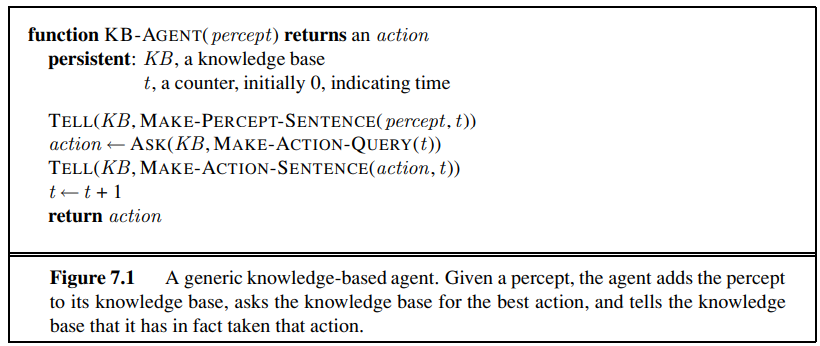
\includegraphics[]{images/KB-agents.png}
\end{center}
The figure above shows the outline of a knowledge-based agent program. Like all our agents, it takes a percept as input and returns an action. The agent maintains a knowledge base, KB, which may initially contain some \textbf{background knowledge}.\newline\newline
Each time the agent program is called, it does three things. First, it TELLs the knowledge base what it perceives. Second, it ASKs the knowledge base what action it should perform. In the process of answering this query, extensive reasoning may be done about the current state of the world, about the outcomes of possible action sequences, and so on.
Third, the agent program TELLs the knowledge base which action was chosen, and the agent executes the action. In order to do so, the agent must be able to:
\begin{itemize}
    \item Represent states, actions, etc.
    \item Incorporate new percepts
    \item Update internal representations of the world
    \item Deduce hidden properties of the world
    \item Deduce appropriate actions
\end{itemize}

\section{The Wumpus world}
In this section we describe an environment in which knowledge-based agents can show their worth. The \textbf{wumpus world} is a cave consisting of rooms connected by passageways. Lurking somewhere in the cave is the terrible wumpus, a beast that eats anyone who enters its room. The wumpus can be shot by an agent, but the agent has only one arrow. Some rooms contain bottomless pits that will trap anyone who wanders into these rooms (except for the wumpus, which is too big to fall in). The only mitigating feature of this bleak environment is the possibility of finding a heap of gold.
\begin{center}
    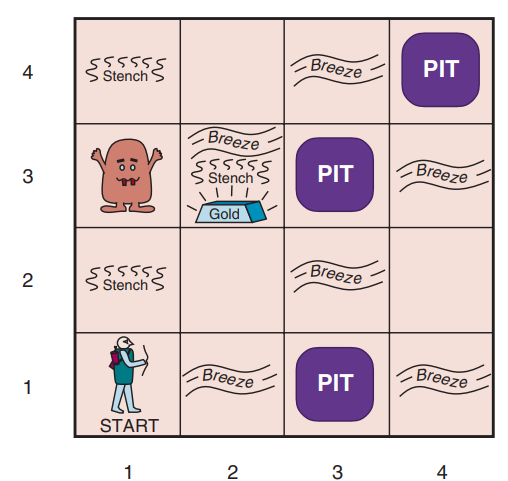
\includegraphics[]{images/wumpus.png}
\end{center}
The precise definition of the task environment is given by the PEAS description:
\begin{itemize}
    \item \textbf{Performance measure}: +1000 for climbing out of the cave with the gold, -1000 for falling into a pit or being eaten by the wumpus, -1 for each action taken and -10 for using up the arrow. The game ends either when the agent dies or when the agent climbs out of the cave.

    \item \textbf{Environment:} A $4 \times 4$ grid of rooms. The agent always starts in the square labeled $[1,1]$, facing to the right. The locations of the gold and the wumpus are chosen randomly, with a uniform distribution, from the squares other than the start square. In addition, each square other than the start can be a pit, with probability 0.2.

    \item \textbf{Actuators:} The agent can move \textit{Forward}, \textit{TurnLeft} by $90^{\circ}$, or \textit{TurnRight} by $90^{\circ}$. The agent dies a miserable death if it enters a square containing a pit or a live wumpus. The action \textit{Grab} can be used to pick up the gold if it is in the same square as the agent. The action \textit{Shoot} can be used to fire an arrow in a straight line in the direction the agent is facing (only one available). Finally, the action \textit{Climb} can be used to climb out of the cave, but only from square $[1,1]$.

    \item \textbf{Sensors:} The agent has five sensors, each of which gives a single bit of information:
    \begin{itemize}
        \item In the square containing the wumpus and in the directly (not diagonally) adjacent squares, the agent will perceive a \textit{Stench}.

        \item In the squares directly adjacent to a pit, the agent will perceive a \textit{Breeze}.

        \item In the square where the gold is, the agent will perceive a \textit{Glitter}.

        \item When an agent walks into a wall, it will perceive a \textit{Bump}.

        \item  When the wumpus is killed, it emits a woeful \textit{Scream} that can be perceived anywhere in the cave.
    \end{itemize}
\end{itemize}
We can characterize the wumpus environment along the various dimensions seen previously. It is discrete, static, and single-agent. It is sequential, because rewards may come only after many actions are taken. It is partially observable, because some aspects of the state are not directly perceivable. For an agent in the environment, the main challenge is its initial ignorance of the configuration of the environment.  Overcoming this ignorance seems to require logical reasoning.\newline\newline
Let us watch a knowledge-based wumpus agent exploring the environment using an informal knowledge representation language consisting of writing
down symbols in a grid:
\begin{center}
    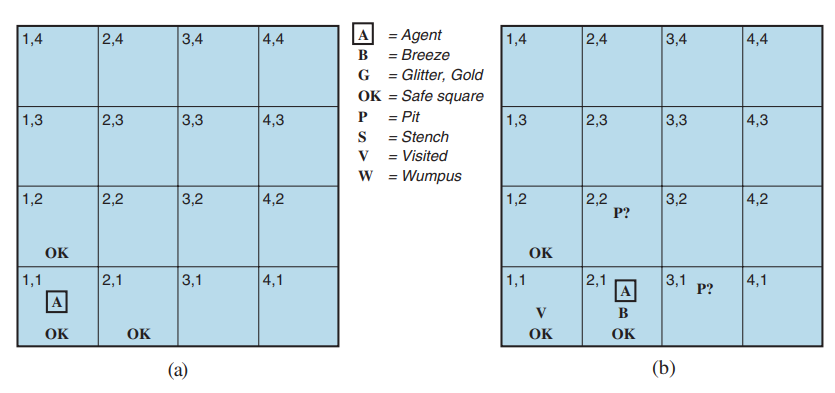
\includegraphics[scale=0.8]{images/wumpus-grid.png}
    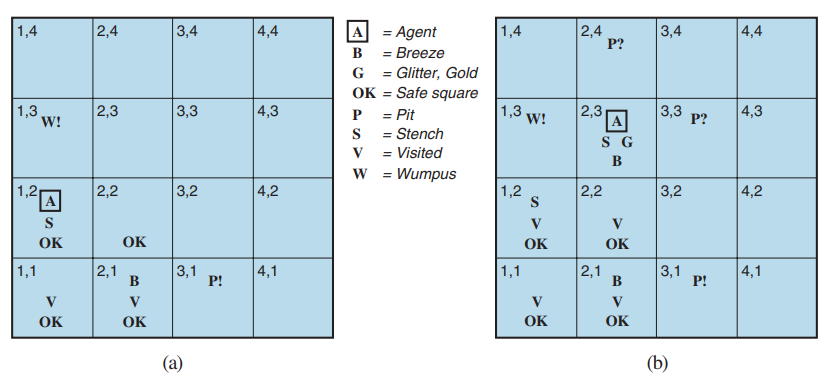
\includegraphics[scale=0.8]{images/wumpus-grid2.png}
\end{center}
Note that in each case for which the agent draws a conclusion from the available information, that conclusion is guaranteed to be correct if the available information is correct. we'll describe how to build logical agents that can represent in a \textbf{formal way} information and draw conclusions.

\section{Propositional Logic}
We now present a simple but powerful logic called \textbf{propositional logic}. The \textbf{syntax} of propositional logic defines the allowable sentences. The \textbf{atomic sentences} consist of a single proposition symbol (P, Q, R, ... but can be whatever). Each such symbol stands for a proposition that can be true or false. There are two proposition symbols with fixed meanings: \textit{True} is the always-true proposition and \textit{False} is the always-false proposition. \textbf{Complex sentences} are constructed from simpler sentences, using parentheses and \textbf{logical connectives}.
\begin{center}
    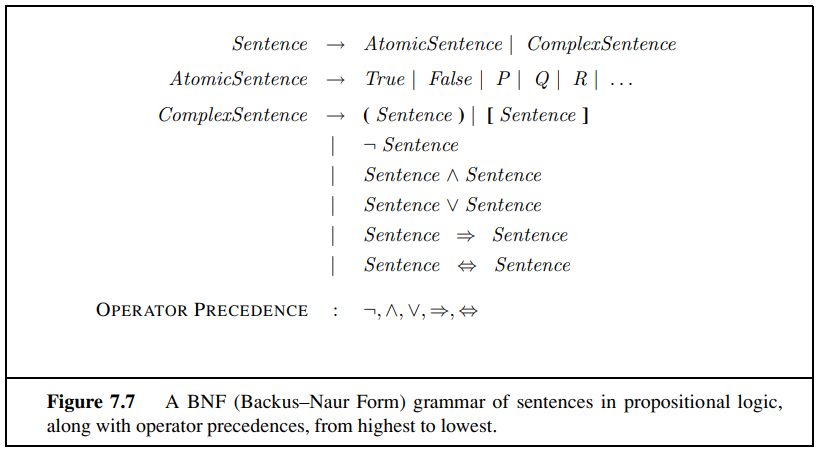
\includegraphics[scale=0.8]{images/BNF.png}
    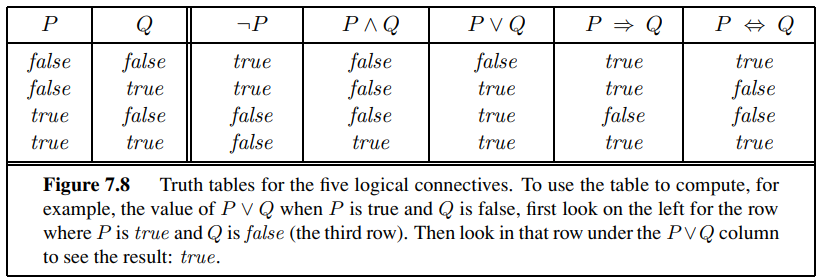
\includegraphics[scale=0.8]{images/truth-table.png}
\end{center}

\section{Models}
As we said previously, the knowledge bases consist of sentences. These sentences are expressed according to the \textbf{syntax} of the representation language, which specifies all the sentences that are well formed. A logic must also define the \textbf{semantics} or meaning of sentences. The semantics defines the truth of each sentence with respect to each possible world.\newline\newline
When we need to be precise, we use the term \textbf{model} in place of “possible world.”  If a sentence $\alpha$ is true in model $m$, we say that $m$ \textbf{satisfies} $\alpha$ or sometimes $m$ \textbf{is a model of} $\alpha$. We use the notation $M(\alpha)$ to mean the set of all models of $\alpha$. Basically, a model assigns truth values to proposition symbols of a sentence.\newline\newline
Now that we have a notion of truth, we are ready to talk about logical reasoning. This involves the relation of logical \textbf{entailment} between sentences, —the idea that a sentence follows logically from another sentence. In mathematical notation, we write:
\[\alpha \vDash \beta\]
to mean that the sentence $\alpha$ entails the sentence $\beta$. The formal definition of entailment is this: $\alpha \vDash \beta$ if and only if, in every model in which $\alpha$ is true, $\beta$ is also true. Using the notation just introduced, we can write
\[\alpha \vDash \beta\,\, \text{if and only if } M(\alpha) \subseteq M(\beta)\]
Note that the direction of the $\subseteq$ means that $\alpha$ is a stronger assertion than $\beta$.\newline\newline
We can apply the same kind of analysis to the wumpus-world reasoning example given previously. The agent has detected nothing in $[1,1]$ and a breeze in $[2,1]$. These percepts, combined with the agent’s knowledge
of the rules of the wumpus world, constitute the KB. The agent is interested (among other things) in whether the adjacent squares $[1,2]$, $[2,2]$, and $[3,1]$ contain pits. Each of the three squares might or might not contain a pit, so (for the purposes of this example) there are $2^3 = 8$ possible models.
\begin{center}
    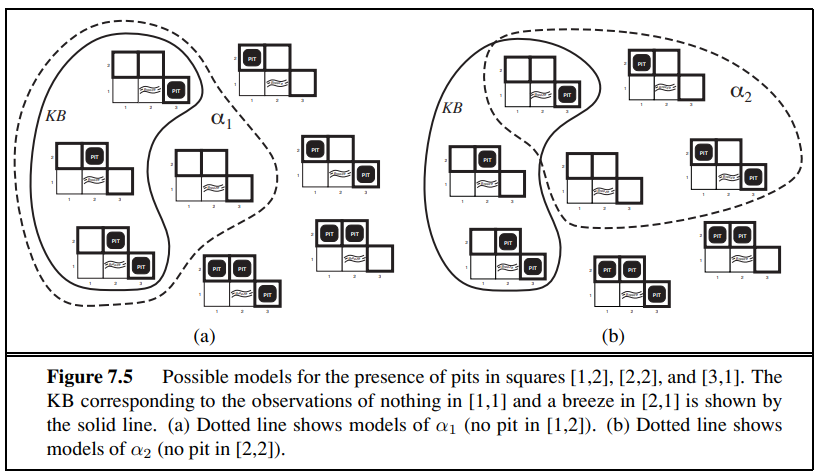
\includegraphics[scale=0.8]{images/kb-wumpus.png}
\end{center}
The KB can be thought of as a set of sentences or as a single sentence that asserts all the individual sentences. The KB is false in models that contradict what the agent knows; for example, the KB is false in any model in which $[1,2]$ contains a pit, because there is no breeze in $[1,1]$. There are in fact just three models in which the KB is true, and these are shown surrounded by a solid line in the figure above.\newline\newline
Now let us consider two possible conclusions:
\begin{itemize}
    \item $\alpha_1 = $ “There is no pit in $[1,2]$.”

    \item $\alpha_2 = $ “There is no pit in $[2,2]$.”

\end{itemize}
By inspection, we see the following: in every model in which KB is true, $\alpha_1$ is also true. Hence $KB \vDash \alpha_1$: there is no pit in $[1,2]$. We can also see that in some models in which KB is true, $\alpha_2$ is false. Hence, the agent cannot conclude that there is no pit in $[2,2]$.\newline\newline
In understanding entailment and inference, it might help to think of the set of all consequences of KB as a haystack and of $\alpha$ as a needle. Entailment is like the needle being in the haystack; inference is like finding it. This distinction is embodied in some formal notation: if an inference algorithm $i$ can derive $\alpha$ from KB, we write:
\[KB \vdash_i \alpha\]
which is pronounced “$\alpha$ is derived from KB by $i$”.\newline\newline
An inference algorithm that derives only entailed sentences is called \textbf{sound}: whenever $KB \vdash_i \alpha$, it is also true that $KB \vDash \alpha$. Note that, as we did with the example before, enumerating all possible models to check that $\alpha$ is true in all models in which KB is true is sound. The property of \textbf{completeness} is also desirable: an inference algorithm is complete if it can derive any sentence that is entailed.\newline\newline
If KB is true in the real world, then any sentence $\alpha$ derived from KB by a sound inference procedure is also true in the real world.

\section{A simple knowledge base}
Now we can construct a knowledge base for the wumpus world, focusing on its immutable aspects. For now, we need the following symbols for each $[x, y]$ location:
\begin{itemize}
    \item $P_{x, y}$ is true if there is a pit in $[x, y]$.
    \item $W_{x,y}$ is true if there is a wumpus in $[x, y]$, dead or alive.
    \item $B_{x,y}$ is true if the agent perceives a breeze in $[x, y]$.
    \item $S_{x,y}$ is true if the agent perceives a stench in $[x, y]$.
\end{itemize}
We label each \textbf{sentence} $R_i$ so that we can refer to them:
\begin{itemize}
    \item There is no pit in $[1,1]$: $R_1:\,\, \neg P_{1,1}$.
    \item A square is breezy if and only if there is a pit in a neighboring square. This has to be stated for each square; for now, we include just the relevant squares:
    \begin{itemize}
        \item $R_2: \,\, B_{1,1} \iff (P_{1,2} \lor P_{2, 1})$
        \item $R_3: \,\, B_{2,1} \iff (P_{1,1} \lor P_{2,2} \lor P_{3,1})$
    \end{itemize}

    \item The preceding sentences are true in all wumpus worlds. Now we include the breeze percepts for the first two squares visited in the specific world the agent is in, leading up to the situation in the figure above (Figure 7.5):
    \begin{itemize}
        \item $R_4: \,\, \neg B_{1,1}$
        \item $R_5: \,\, B_{2,1}$
    \end{itemize}
\end{itemize}
Our goal now is to decide whether $KB \vDash \alpha$ for some sentence $\alpha$. For example, is $\neg P_{1,2}$ entailed by our KB? Our first algorithm for inference is a \textbf{model-checking} approach that is a direct implementation of the definition of entailment: enumerate the models, and check that $\alpha$ is true in every model in which KB is true.
\begin{center}
    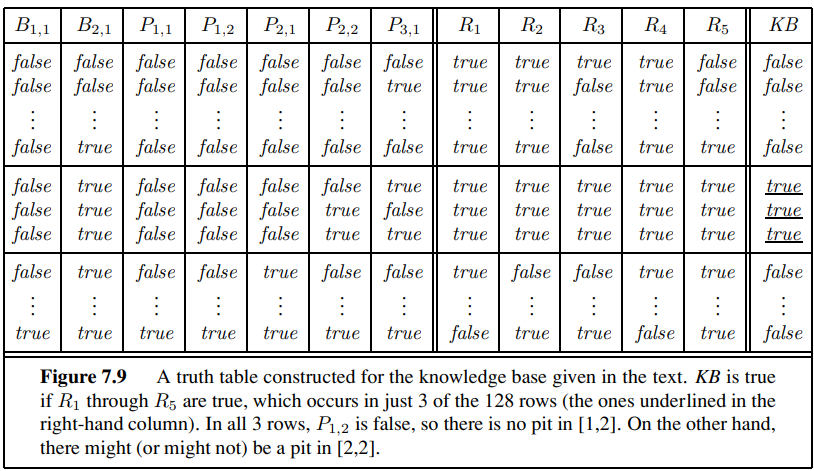
\includegraphics[]{images/wumpus-table.png}
\end{center}
Returning to our wumpus-world example, the relevant proposition \textbf{symbols} are $B_{1,1}, B_{2,1}, P_{1,1}, P_{1,2}, P_{2,1}, P_{2,2}$, and $P_{3,1}$. With seven symbols, there are $2^7 = 128$ possible models; in three of these, KB is true. Note that this is just a "snapshot" of the situation shown in the Figure 7.5. Obviously, as the agent goes on, the KB changes. In the three model where KB is \textit{True}, $\neg P_{1,2}$ is also \textit{True}. Hence, there is no pit in $[1,2]$. On the other hand, $P_{2,2}$ is true in two of the three models and false in one, so we cannot yet tell whether there is a pit in $[2,2]$. Note that KB is true if $R_1$ through $R_5$ are true (KB can be expressed as a sentence $R_1 \land ... \land R_5$), which occurs in just 3 of the 128 rows.
\begin{center}
    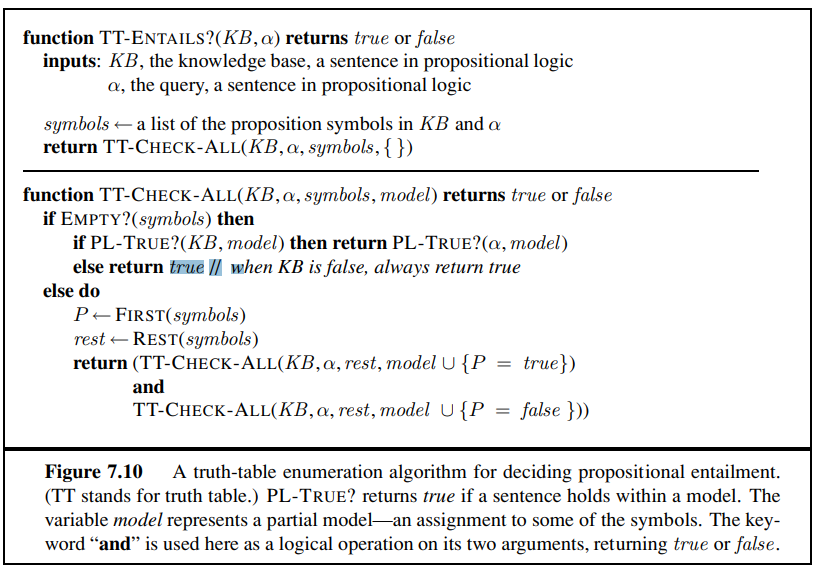
\includegraphics[]{images/tt-algorithm.png}
\end{center}
The algorithm above performs a recursive enumeration of a finite space of assignments to symbols. The algorithm is \textbf{sound} because it implements directly the definition of entailment, and \textbf{complete} because it works for any KB and $\alpha$ and always terminates; there are only finitely many models to examine.\newline\newline
Basically, the algorithm constructs the truth table seen above using a recursive implementation. In particular, it creates a binary tree where the nodes are the symbols in the KB and the branches are truth assignment for that symbol (\textit{True} or \textit{False}). It starts from the first symbol and recursively produces all the possible assignment for all the possible symbols. The paths from the root to the leaves corresponds to the rows of the table above, i.e. the models. Once the algorithm arrives at a leaf, it checks whether the sentence $\alpha$ holds within the corresponding model (path). The algorithm returns always \textit{True} if the KB is \textit{False} w.r.t the model because we are only interested to see if a sentence is \textit{True} when the KB is \textit{True}. These operations correspond to look at the rows of the table (models) where KB is \textit{True} and check whether $\alpha$ is also \textit{True}. If the sentence $\alpha$ is \textit{True} for all the models where also KB is \textit{True} (i.e. all the leaves \textit{returns} \textit{True}), then $\alpha$ can be deduces from KB. Note that if all the leaves return \textit{True}, when the algorithm ascents from recursion, the \textit{True} value is propagated towards the root by the logical \textit{and} and eventually the algorithm returns \textit{True}.  For the same reason, it is sufficient that just one leaf returns \textit{False} that the whole algorithm returns \textit{False} (this is why the algorithms always returns \textit{True} when KB is \textit{False}).\newline\newline
Note that If KB and $\alpha$ contain $n$ symbols in all, then there are $2^n$ models. Thus, the time complexity of the algorithm is $O(2^n)$ (The space complexity is only $O(n)$ because the enumeration is depth-first). Unfortunately, propositional entailment is co-NP-complete.

\chapter{Lec 09 - Neural Networks III}

\section{Other activation functions}
Multiple layers of cascaded units makes a Neural Network able to implement complex non linear functions. The non linearity of the model is given by the activation functions. In fact, without them (linear activation) the result of the model, even if it’s very complex, would still be linear. If we used step activation functions we wouldn't be able to resort to gradient descent to optimize the weights. This is because step function is not derivable. We have to choose one or more activation functions that are derivable.
\begin{itemize}
    \item \textbf{Sigmoid:}
    \[\sigma(y) = \frac{1}{1 + e^{-y}}\]

    \item \textbf{ReLu:}
    \[r(y) = max(0, y)\]
\end{itemize}
\section{Multi-layer Neural Networks: Keywords}
Let's define the most important keywords for Multi-layer Neural Networks:
\begin{itemize}
    \item $d$ \textbf{input units}: $d$ input data size $\textbf{x} \equiv (x_{1},...,x_{d})$, $d + 1$ when including the bias in the weight vector $\textbf{x}^{'} \equiv (x_{0}, x_{1},...,x_{d})$

    \item $n_{H}$ \textbf{hidden units} (with output $\textbf{y} \equiv (y_{1},...,y_{n_{H}})$)

    \item $c$ \textbf{output units}: $\textbf{z} \equiv (z_{1},...,z_{c})$. The number of desired output is $\textbf{t} \equiv (t_{1},...,t_{c})$

    \item $w_{ji}$ weight from the $i$-th input unit to the $j$-th hidden unit ($w_{j}$ is the weight vector of the $j$-th hidden unit)

    \item $w_{kj}$ weight from the $j$-th hidden unit to the $k$-th output unit ($w_{k}$ is the weight vector of the $k$-th output unit)
\end{itemize}
\section{Learning algorithm}
Let's consider, for example, a Neural Network with just one hidden layer and \textbf{sigmoid activation functions}. The basic idea of the learning algorithm consists in two phases:
\begin{itemize}
    \item \textbf{Forward phase:} for each example in the training set, present it to the network and compute the output.
    \item \textbf{Backward phase:} Back-propagate the committed error and update the weights of the hidden units accordingly. 
\end{itemize}
This algorithm is called \textbf{Backpropagation}\newline\newline
As we said before, this algorithm is based on gradient descent, so we need to minimize an error function $E[\textbf{w}]$ that can be defined as follows:
\[E[\textbf{w}] = \frac{1}{2cN}\sum_{s=1}^{N}\sum_{k=1}^{c}(t_{k}^{(s)} - z_{k}^{(s)})^{2}\]
In order to implement Backpropagation, we need to first compute the gradient for the weights of both output and hidden units.
\begin{itemize}
    \item \textbf{Gradient of the weights of an output unit:}
    \[\frac{\partial E}{\partial w_{\hat{k}\hat{j}}} = - \frac{1}{cN}\sum_{s=1}^{N}(t_{\hat{k}}^{(s)} - z_{\hat{k}}^{(s)} )z_{\hat{k}}(1 - z_{\hat{k}})y_{\hat{j}}^{(s)}\]
    where $y_{\hat{j}}^{(s)}$ is the output of the $\hat{j}$-th hidden unit.
    
    \item \textbf{Gradient of the weights of a hidden unit:}
    \[\frac{\partial E}{\partial w_{\hat{j}\hat{i}}} = - \frac{1}{cN}\sum_{s=1}^{N}y_{\hat{j}}^{(s)}(1 - y_{\hat{j}}^{(s)})x_{\hat{i}}^{(s)}\sum_{k=1}^{c}(t_{\hat{k}}^{(s)} - z_{\hat{k}}^{(s)} )z_{\hat{k}}(1 - z_{\hat{k}})w_{k\hat{j}}\]
\end{itemize}
Note that, for simplicity, we are considering a Neural Network with just one hidden layer, but the derivation can be extended for more than one hidden layer.
\subsection{Back-propagation algorithm}
Back-propagation is an algorithm that aims to update the weights of a Neural Network in order to minimize the error between the predicted output and the true output. The algorithm works by propagating the error back through the network, starting with the output layer and moving backwards through the hidden layers, adjusting the weights at each layer to reduce the error. It can be implemented in different ways:
\begin{itemize}
    \item \textbf{Batch gradient descent:} It \textbf{cumulates} gradients over all the training examples and then updates the weights.
    \item \textbf{Stochastic gradient descent:} For each example in $S$, it computes the gradients and update the weights.
    \item \textbf{Mini-batch gradient descent:} It updates the weights considering a subset of examples $Q \subseteq S$. 
\end{itemize}
This process is typically repeated many times until the error is sufficiently small or the maximum number of iterations is reached. Let's define the algorithm according to the derivations seen before:\newline\newline
\textbf{Back-propagation (stochastic)}
\begin{enumerate}
    \item Initialize all weights with small random values (e.g. between -0.5 and +0.5)
    \item Until the termination condition is satisfied:
    \begin{enumerate}
        \item For each $(\textbf{x},\textbf{t}) \in S$:
        \begin{enumerate}
            \item Present $\textbf{x}$ to the net and compute the vectors $\textbf{y}$ and $\textbf{z}$
            \item For each output unit $k$:
            \[\delta_{k} = z_{k}(1 - z_{k})(t_{k} - z_{k})\]
            \[\Delta w_{kj} = \delta_{k}y_{j}\]

            \item For each hidden unit $j$:
            \[\delta_{j} = y_{j}(1 - y_{j})\sum_{k=1}^{c}w_{kj}\delta_{k}\]
            \[\Delta w_{ji} = \delta_{j}x_{i}\]

            \item Update all weights:
            \[w_{sq} \leftarrow w_{sq} + \eta \Delta w_{sq}\]
        \end{enumerate}
    \end{enumerate}
\end{enumerate}
Note that this algorithm works only for a network with one hidden layer, but can be easily extended. In fact, the algorithm computes the error term $\delta$ for each unit of each layer, and then it multiplies this error term for the input of the unit.

\section{Computational power of neural networks}
\textbf{Theorem (Pinkus, 1996) simplified}:\newline
Given a feed-forward NN with just one hiddel layer, any continuous function $f:\mathbb{R}^{n} \rightarrow \mathbb{R}$ and an arbitrarily small $\epsilon > 0$, then, for a large class of activation functions, there always exists an integer $M$ such that the function $g: \mathbb{R}^{n} \rightarrow \mathbb{R}$ computed by the net using at least $M$ hidden units approximates the function $f$ with tolerance $\epsilon$, that is:
\[max_{x \in \Omega}|f(\textbf{x}) - g(\textbf{x})| < \epsilon\]
Note that the theorem attests the existence of a NN with $M$ hidden units that approximates the target function with the desired tolerance, but it says nothing about how $M$ can be computed.

\section{Fine tuning neural networks}
The choice of the net typology determines the hypothesis space used. With three-layers architecture (input, hidden, output), the number of hidden units detrmines the complexity of the hypothesis space. As we said for the Perceptron, the choice of the learning rate $\eta$ can be crucial for the convergence.
\subsection{Avoiding local minima}
The local minima problem in neural networks refers to the scenario where a neural network gets stuck in a sub-optimal solution during the training process. Instead of reaching the global minimum, which is the best possible solution, the network settles for a local minimum, that may not be the best fit for the data. This can happen because the loss function used can have multiple local minima, and the optimization algorithm may only find one of them. In order to avoid this problem, we can use different techniques:
\begin{itemize}
    \item Adding a term to the weight update rule (called \textbf{momentum}). Basically, a contribution deriving from the previous step is added, imposing a kind of inertia on the system.

    \item Using \textbf{stochastic training} (randomizing on the examples) instead of batch training can facilitate to avoid local minima.

    \item \textbf{Training multiple NNs} on the same data with different initialization and combining the outputs.
\end{itemize}

\subsection{Over-fitting}
With neural networks, usually, the error on the validation set increases as the number of weight updates increases. This is because, at the beginning, with small absolute values of the weights (similar each other), the decision surfaces are \textit{smoother}. When the absolute values of the weights increase , the complexity of the decision surfaces increases and with it the possibility to suffer over-fitting. \newline\newline
A possible solution can be to use an additional term in the error function to minimize based on the norm of the weights (regularization) $E + ||w||^{2}$.

\section{Hidden layer representation}
An important feature of multi-layer NNs is that they can find useful representations of input data (alternative to the input representation). Specifically, the output of the hidden units is an effective new input representation for the next layers. This feature can be used to define a particular type of NNs called Auto-encoders.


\chapter{Lec 10 - Generalized Linear Models and SVM I}
\section{Linear Models}
Linear models are one of the most important types of models in machine learning. A linear model is of the form:
\[f_{\textbf{w},b}(\textbf{x}) = \sum_{i=1}^{m} w_{i}x_{i} + b = \textbf{w} \cdot \textbf{x} + b\]
Which can also be written as
\[f_{\textbf{w},b}(\textbf{x}) = \sum_{i=0}^{m} w_{i}x_{i}= \textbf{w} \cdot \textbf{x}\]
where $x_{0} = 1$.
\begin{itemize}
    \item For \textbf{classification}, the sign of the result is returned, that is:
    \[h(\textbf{x}) = sign(f_{\textbf{w}}) \in \{-1, +1\}\]

    \item For \textbf{regression}, the \textit{original} function can be taken, that is:
    \[h(\textbf{x}) = f_{\textbf{w}} \in \mathbb{R}\]
\end{itemize}
\subsection{Linear Regression}
Given a training set $S = \{(\textbf{x}_{1}, y_{1}), ..., (\textbf{x}_{n}, y_{n})\}$, in linear regression we look for a hypothesis $h_{\textbf{w}}$ which minimizes the mean squared error on the training set, that is:
\[argmin_{\textbf{w}} \frac{1}{n}\sum_{i=0}^{n}(h_{\textbf{w}}(\textbf{x}_{i}) - y_{i})^{2}\]
We can formalize it in matrices terms:
\[E(\textbf{w}) = \frac{1}{n}\sum_{i=0}^{n}(h_{\textbf{w}}(\textbf{x}_{i}) - y_{i})^{2}\]
\[= \frac{1}{n}\sum_{i=0}^{n}(\textbf{w} \cdot \textbf{x}_{i} - y_{i})^{2}\]
\[= \frac{1}{n}||\textbf{Xw} - \textbf{y}||\]
where:
\begin{itemize}
    \item $\textbf{X}$ is a matrix of size $n \times d$
    \item $\textbf{w}$ is a vector of size $d \times 1$
    \item $\textbf{y}$ is a vector of size $n \times 1$
\end{itemize}
$d$ is the dimension of the feature space (including the bias term). Basically, we want that $\textbf{Xw} \approx \textbf{y}$.\newline\newline
Since $||\vec{z}||^{2} = \sum_{i}z_{i}^{2}$, the optimization problem can be defined as follows:
\[min_{\textbf{w}}E(\textbf{w}) \equiv \frac{1}{n}||\textbf{Xw} - \textbf{y}||^{2}\]
We want to find the vector $\textbf{w}$ that minimizes $E$. Basically, we want to find the points $\textbf{w}$ where the gradient vanishes (equals to 0), that is:
\[\nabla E(\textbf{w}) = \frac{2}{n}\textbf{X}^{T} (\textbf{Xw} - \textbf{y}) = 0\]
\[\textbf{X}^{T}\textbf{Xw} = \textbf{X}^{T}\textbf{y}\]
By multiplying the quantity $(\textbf{X}^{T}\textbf{X})^{-1}$ both on the left and on the right of the equation, it becomes:
\[(\textbf{X}^{T}\textbf{X})^{-1}(\textbf{X}^{T}\textbf{X})\textbf{w} = (\textbf{X}^{T}\textbf{X})^{-1}\textbf{X}^{T}\textbf{y}\]
Since $(\textbf{X}^{T}\textbf{X})^{-1}(\textbf{X}^{T}\textbf{X})$ is the identity matrix, the final equation is:
\[\textbf{w} = (\textbf{X}^{T}\textbf{X})^{-1}\textbf{X}^{T}\textbf{y}\]
This is a \textbf{closed form solution}. It means that with just one computation we are able to find the solution, it's not am iterative process. However, computing the inverse of a matrix can be very computational inefficient.

\subsection{Non-linear mapping}
The goal of non-linear mapping is to apply a transformation to non-linearly separable points in order to map them in a new feature space that is linearly separable. Then, a linear model (hyperplane) in the transformed space will correspond to a non-linear decision surface in the original space (Generalized Linear Models).

\section{Linear separability}
Consider the hypothesis space of hyperplanes. Given a set of linearly separable points, we have different hyperplanes that separates them. Intuitively, the widest possible margin (or \textbf{optimal}) hyperplane is the best one, because is the one that generalizes better, but how can we compute to which $\textbf{w}$, $b$ the best hyperplane corresponds.
\subsection{Margin of a hyperplane}
The margin of a hyperplane is the distance between the hyperplane and the closest data points of each class. \newline\newline
Let's consider the \textbf{binary classification} problem. Given the hyperplane $\textbf{w} \cdot \textbf{x} + b = 0$ (\textbf{optimal hyperplane}), the \textit{"distance"} of a point $\textbf{x}$ from the hyperplane can be expressed by the algebraic measure $g(\textbf{x}) = \textbf{w}^{T} \cdot \textbf{x} + b$. We can write $\textbf{x}$ as follows:
\[\textbf{x} = \textbf{x}_{p} + r\frac{\textbf{w}}{||\textbf{w}||}\]
where:
\begin{itemize}
    \item $||\textbf{w}||$ is the norm of $\textbf{w}$
    \item $\textbf{x}_{p}$ is the normal projection of $\textbf{x}$ onto the hyperplane.
    \item $r$ is the desired algebraic distance ($r > 0$ if $\textbf{x}$ is on the positive side of the hyperplane, otherwise $r < 0$).
\end{itemize}
Note that $g(\textbf{x}_{p}) = 0$ because $\textbf{x}_{p}$ is on the hyperplane. Furthermore, since we are considering the optimal hyperplane, the absolute distance between this hyperplane and any nearest positive example is the same as the absolute distance between any negative example. So, we can \textit{normalize} the value of $g$ such that $g(\textbf{x}) = 1$ if $\textbf{x}$ is in the positive margin hyperplane and $g(\textbf{x}) = -1$ if $\textbf{x}$ is in the negative margin hyperplane.\newline\newline
Take $\textbf{x}_{k}$ in the positive margin hyperplane, it follows that
\[g(\textbf{x}_{k}) = \textbf{w}^{T}\textbf{x}_{k} + b\]
Since $\textbf{x}_{k} = \textbf{x}_{p} + r\frac{\textbf{w}}{||\textbf{w}||}$:
\[= \textbf{w}^{T}\left(\textbf{x}_{p} + r\frac{\textbf{w}}{||\textbf{w}||}\right) + b\]
\[= \textbf{w}^{T}\textbf{x}_{p} + b + r\frac{\textbf{w}^{T}\textbf{w}}{||\textbf{w}||}\]
Since $\textbf{w}^{T}\textbf{w} = ||\textbf{w}||^{2}$:
\[= \textbf{w}^{T}\textbf{x}_{p} + b + r||\textbf{w}||\]
The term $\textbf{w}^{T}\textbf{x}_{p} + b = 0$ because, as we said before, $g(\textbf{x}_{p}) = 0$. This implies that:
\[g(\textbf{x}_{k}) = r||\textbf{w}|| = +1\]
This is true only if
\[r = \frac{1}{||\textbf{w}||}\]
Then, the margin $\rho$ is defined as follows:
\[\rho = 2r = \frac{2}{||\textbf{w}||}\]
\section{Support Vector Machines (SVM)}
Support Vector Machines (SVMs) are a set of supervised learning methods used for classification and regression tasks. The idea behind SVMs is to find the best hyperplane that separates the training data. This hyperplane is chosen in such a way that it maximizes the margin.
\subsection{Separable case: Quadratic optimization}
If we have $n$ linearly separable examples $\{(\textbf{x}_{i}, y_{i})\}$ (binary classification), it is possible to find the optimal hyperplane $h(\textbf{x}) = sign(\textbf{w} \cdot \textbf{x} + b)$ by solving the following \textbf{constrained} quadratic optimization problem:
\[min_{\textbf{w},b}\frac{1}{2}||\textbf{w}||^{2}\]
\[subject \,\, to: \,\, \forall i \in \{1,...,n\}: y_{i}(\textbf{w} \cdot \textbf{x}_{i} + b) \geq 1\]
Since the margin is defined as $\rho = \frac{2}{||\textbf{w}||}$ and we want to maximize it, we need to minimize $||\textbf{w}||$. This minimization problem is subject to the constraint that each point in the training set must be on the \textit{correct} side of the hyperplane, which means that for each point, the following inequality must hold: $\forall i \in \{1,...,n\}: y_{i}(\textbf{w} \cdot \textbf{x}_{i} + b) \geq 1$. This constraint is given by the fact that:
\begin{itemize}
    \item $\textbf{w} \cdot \textbf{x}_{i} + b \geq 1$ if $y_{i} = +1$
    \item $\textbf{w} \cdot \textbf{x}_{i} + b \leq 1$ if $y_{i} = -1$
\end{itemize}
This is a \textbf{convex} constrained quadratic problem, and for this reason it guarantees a unique solution.\newline\newline
With a large number of features it can be computationally inefficient to solve this problem, so we can use its \textbf{dual formulation}
\subsection{Dual formulation}
In the dual problem, Lagrange multipliers $\alpha_{i} \geq 0$ are associated with every constraint in the primal problem (one for each example).
\[max_{\alpha} \sum_{i=1}^{n}\alpha_{i} - \frac{1}{2}\sum_{i,j=1}^{n}y_{i}y_{j}\alpha_{i}\alpha_{j}(\textbf{x}_{i} \cdot \textbf{x}_{j})\]
\[subject \,\, to: \,\, \forall i \in \{1,...,n\}: \,\, \alpha_{i} \geq 0 \,\, and \,\, \sum_{i=1}^{n}y_{i}\alpha_{i} = 0\]
At the solution, most of the $\alpha_{i}$'s are zeros. Those examples associated with non zero multipliers are called \textbf{support vectors}.

\subsection{SVM solution}
The primal solution turns out to be:
\[\textbf{w} = \sum_{i=1}^{n}y_{i}\alpha_{i}\textbf{x}_{i}\]
\[b = y_{k} - \textbf{w} \cdot \textbf{x}_{k}\,\, \forall \textbf{x}_{k}\,\,s.t\,\, \alpha_{k} > 0\]
Hence:
\[h(\textbf{x}) = sign(\textbf{w} \cdot \textbf{x} + b) = sign\left(\sum_{i = 1 \in support \,\, vector}^{n}y_{i}\alpha_{i}(\textbf{x}_{i} \cdot \textbf{x}) + b\right)\]
The decision function only depends on dot products between the point and othe points in the training set (the support vectors).

\chapter{Lec 11 - NP-Hardness}

\section{Tractable vs Intractable problems}
Problems for which a polynomial algorithm exists are called \textbf{tractable}. If no such algorithm exists, the problem is called \textbf{intractable}.\newline\newline
\textbf{Examples:}
\begin{enumerate}
    \item \textbf{Eulerian circuit problem:} Given an undirected graph, an Eulerian circuit is a cycle that traverses all the edges only once. This problem can be solved in linear time. Note that in an Euler circuit you might pass through a vertex more than once.

    \item \textbf{Hamiltonian circuit problem:} Given an undirected graph, an Hamiltonian circuit is a cycle that traverses all the vertices only once. To date, no one knows a polynomial algorithm to solve it. Note that in a Hamiltonian circuit you may not pass through all edges.

    \item \textbf{Minimum spanning tree:}

    \item \textbf{Traveling Salesperson Problem (TSP):} Given a complete, undirected graph and a function $w: E \rightarrow \mathbb{R}$, output a \textbf{tour} (i.e. a cycle that visits every vertex exactly once) of minimum cost
    \[T \subseteq E \quad \text{minimizing }\sum_{e \in T}w(e)\]
    To date, no one knows a polynomial algorithm to solve it.
\end{enumerate}
A much easier task can be the following: Given a graph and a list of vertices $C$, \textbf{check} if $C$ is an Hamiltonian circuit.\newline\newline
Problems that are \textit{easy} to solve belong to the \textbf{complexity class} \textbf{P} (\textit{polynomial time}), 1), 3) $\in$ \textbf{P}. Problems that are \textit{easy} to verify belong to the complexity class \textbf{NP} (\textit{Non-deterministic polynomial}), 1), 2) ,3) ,4) $\in$ \textbf{NP}.

\section{NP-Hard}
\textbf{Decision Problems:}\newline
To simplify the study of the complexity of problems, we limit our attention to problems with a boolean answer (YES, NO), that is, decision problems.\newline\newline
Let's define \textbf{P} and \textbf{NP} classes in a more formal way:
\begin{itemize}
    \item \textbf{P} is the set of decision problems that can be solved in polynomial time.

    \item \textbf{NP} is the set of decision problems with the following property: if the answer is YES, then there is a proof of this fact that can be checked in polynomial time.

    \item \textbf{NP-Hard:} A computational problem is \textbf{NP-Hard} if a polynomial-time algorithm that solves it would imply a polynomial-time algorithm that solves every problem in \textbf{NP}.\newline\newline
    A problem is \textbf{NP-Complete} if it is both in \textbf{NP} and \textbf{NP-Hard}. Basically, these problems are the hardest in \textbf{NP}. 
\end{itemize}
\begin{figure}[h]
    \centering
    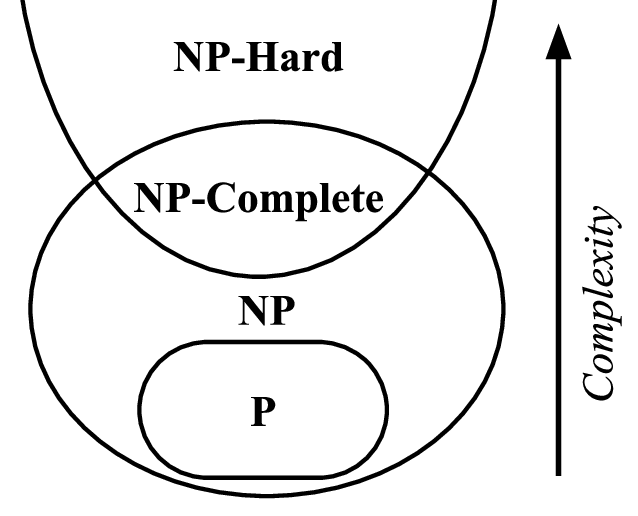
\includegraphics[scale=0.4]{images/P-NP.png}
    \caption{What we think the computation classes look like}
    \label{fig:P-NP-Np-Hard}
\end{figure}
One of the main open questions in computer science is whether \textbf{P=NP}.\newline\newline
Studying NP-Hardness is important because if a problem is \textbf{NP-Hard} is a strong evidence that it is intractable. It suggests you to use a different approach, such as identify tractable special-cases, or use \textbf{approximation algorithms}.

\section{Cook-Levin Theorem}
\textit{In computational complexity theory, the Cook–Levin theorem, also known as Cook's theorem, states that the Boolean satisfiability problem is \textbf{NP-complete}.}\footnote{Wikipedia definition}\newline\newline
SAT: formula satisfiability:
\begin{itemize}
    \item input: A boolean formula like the following: $(b \land \neg c) \lor (\neg a \land b)$

    \item output: It is possible to assign boolean values to the variables $a, b, c, ...$ such that the entire formula evaluates to TRUE?
\end{itemize}
determining the satisfiability of a formula in conjunctive normal form (CNF) where each clause is limited to at most three literals is \textbf{NP-complete} also; this problem is called \textbf{3-SAT}.\newline\newline
\textbf{Example of 3-CNF formula:}
\[(a \lor b \lor c) \land (b \lor \neg c \lor \neg d) \land (\neg a \lor c \lor d)\]
%Check if the theorem was defined on 3SAT???
How can we show that a problem is \textbf{NP-Hard}?

\section{Reductions}

To prove that a problem $P$ is \textbf{NP-Hard} we use \textbf{reduction}. We want to prove that every problem in \textbf{NP} reduces to problem $P$.\newline\newline
Reducing problem $A$ to problem $B$ means describing an algorithm to solve $A$ under the assumption that an algorithm for $B$ exists.
\begin{center}
    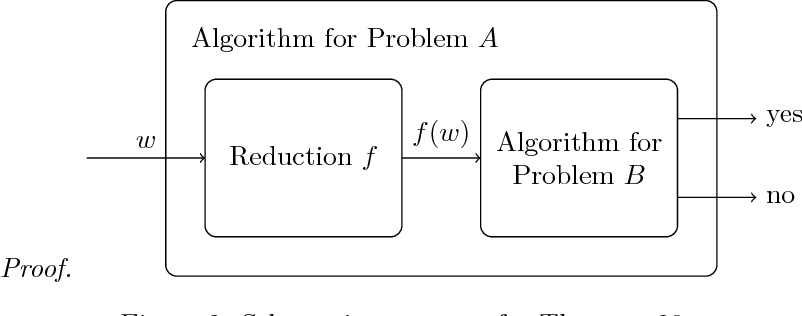
\includegraphics[scale=0.4]{images/Reduction.png}
\end{center}
$A < B$ means \textit{A reduces to B} where $B$ is the hardest problem ($A$ is as hard as $B$).


\chapter{Lec 12 - Preprocessing}

\section{Supervised learning pipeline}
The supervised learning pipeline can be summarized as follows:
\begin{enumerate}
    \item Analysis of the problem (Classification, Regression, ...)

    \item Collection, analysis and cleaning data

    \item Pre-processing and managing missing values

    \item Study of correlation between variables 

    \item Feature selection/weighting/learning

    \item Choice of the predictor and model selection

    \item Test
\end{enumerate}
Some of the most common objects that we can find in machine learning are:
\begin{itemize}
    \item \textbf{Vectors} (Set of values)
    \item \textbf{Strings}
    \item \textbf{Sets and Bags}: for example, the set of terms in a document or their frequency
    \item \textbf{Tensors}: for example, images and video
    \item \textbf{Trees and graphs}
\end{itemize}
The easiest way to represent these objects is to map them in a vectorial representation.\newline\newline
Features values can be divided in two classes: \textbf{Categorical} and \textbf{Quantitative}:
\begin{itemize}
    \item Categorical or symbolic features
    \begin{itemize}
        \item Nominals: They are used for naming or labeling variables, without any quantitative value. There is usually no intrinsic ordering to nominal data.

        \item Ordinals: Is a type of categorical data with an order.
    \end{itemize}

    \item Quantitative and numeric features:
    \begin{itemize}
        \item Intervals (Enumerables)
        \item Ration (Real values)
    \end{itemize}
\end{itemize}
Let's see how to encode categorical and quantitative variables into a vector.

\section{Encoding categorical or symbolic variables}
One of the most common method to encode a categorical variable into a vector is the \textbf{OneHot Encoding}. This technique allows you to represents categorical variables in a vector with as many components as the number of possible values for the variable.\newline\newline
For example, let's say that we want to encode a variable corresponding to the brand of a car. The possible values that an instance can take are: \textit{(Fiat, Toyota, Ford)}. The OneHot encoding of an instance having \textit{Toyota} as brand value could be the following: $[0, 1, 0]$. Basically, it's a vector where we set to one the component corresponding to the value of the instance.

\section{Encoding of continuous variables}
In this case, it is more difficult to find a good mapping. Therefore, the features are typically transformed to obtain values \textit{comparable} with other features.\newline\newline
Given a matrix of instances (training set), for each feature $j$, let $\hat{x}_{j} = \frac{1}{n}\sum_{i=1}^{n}x_{ij}$ be the average value of the current feature and let $\sigma_{j} = \sqrt{\frac{1}{n}\sum_{i=1}^{n}(x_{ij} - \hat{x}_{j})^{2}}$ be the standard deviation of $j$. We can apply the following transformations:
\begin{itemize}
    \item Centering: $c(x_{ij}) = x_{ij} - \hat{x}_{j}$. For each value $x_{ij}$ we compute $c(x_{ij})$ which is equal to the difference between the value and the average of the corresponding feature.

    \item Standardization: $s(x_{ij}) = \frac{c(x_{ij})}{\sigma_{j}}$. We want the \textit{columns} (features) of the matrix to have mean equals to 0 and variance equals to 1.

    \item Scaling to a range: $h(x_{ij}) = \frac{x_{ij} - x_{min j}}{x_{max j} - x_{min j}}$. Each value is scaled in a range between 0 and 1.

    \item Normalization: $g(\textbf{x}) = \frac{\textbf{x}}{||\textbf{x}||}$. In this case, we don't work over features but we want to normalize the instances (rows).
\end{itemize}
The python module \textit{sklearn} provides several methods to perform this kind of pre-processing.

\subsection{K-Nearest Neighbors}
K-Nearest Neighbors is a simple classification algorithm where a test example is classified with the majority class of its k-neighbors in the training set.\newline\newline
When the instances are \textbf{normalized} we can define the squared distance between them in terms of dot-product:
\[||\textbf{x} - \textbf{z}||^{2}\]
\[= ||\textbf{x}||^{2} + ||\textbf{z}||^{2} - 2\langle \textbf{x}, \textbf{z}  \rangle\]
Since the norm of the instances is equal to 1, it follows that:
\[= 2 - 2\langle \textbf{x}, \textbf{z}  \rangle\]
So, with normalized data, the distance between two instances is inversely proportional to their dot-product.

\section{Feature selection and feature extraction}
Feature \textbf{selection} is the reduction of the dimensionality of the features obtained by removing irrelevant or redundant features. The interpretability of the model is maintained.\newline\newline
Feature \textbf{extraction} is the reduction of the dimensionality of the features obtained by combining the original features (e.g. PCA). Generally, the interpretability of the model is lost.

\subsection{Feature selection}
The top reasons to use feature selection are:
\begin{itemize}
    \item It enables the machine learning algorithm to train faster

    \item It reduces the complexity of a model and makes it easier to interpret.

    \item It improves the accuracy of a model if the right subset is chosen.

    \item It reduces over-fitting.
\end{itemize}
Feature selection methods can be divided in 3 classes:
\begin{itemize}
    \item \textbf{Filter methods:} They perform feature selection before applying the predictor. They use an efficient scoring function (e.g. Mutual information, Chi squared, Information gain) that determines the usefulness of a given set of features.

    \item \textbf{Wrapped methods:} The predictor is evaluated on a hold-out sample using subset of different features. Then, the subset with highest score is chosen.

    \item \textbf{Embedded methods:} The selection of features occurs in conjunction with the training of the model, for example, by modifying the objective function to be optimized. 
\end{itemize}

\subsection{Feature extraction (PCA)}
\textbf{Principal Component Analysis (PCA)} converts a set of instances with possibly related features into corresponding values on another set of linearly unrelated features (principal components).\newline\newline
\textbf{Neural Networks} can also be seen as a particular way to perform feature extraction on their hidden layers. In fact, the output values of one of the hidden layers can be considered as a new representation of the original data.


\chapter{Lec 13 - Resolution for First Order Logic}

\section{Resolution}
The last of our three families of logical systems is based on \textbf{resolution}. In resolution for first order logic two clauses, which are assumed to be standardized apart so
that they share no variables, can be resolved if they contain complementary literals. Propositional literals are complementary if one is the negation of the other; first-order literals are complementary if one unifies with the negation of the other. Thus, we have
\begin{center}
    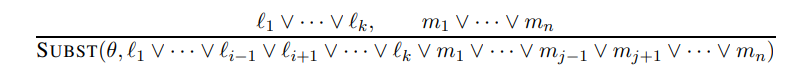
\includegraphics[]{images/resolution-fol.png}
\end{center}
where $UNIFY(l_i,\neg{m_j} ) = \theta$. For example, we can resolve the two clauses
\[[Animal(F(x)) \lor Loves(G(x), x)]\,\, \text{and} \,\,[\neg Loves(u, v) \lor \neg Kills(u, v)]\]
by eliminating the complementary literals $Loves(G(x), x)$ and $\neg Loves(u, v)$, with unifier $\theta = \{u/G(x), v/x\}$, to produce the \textbf{resolvent} clause
\[[Animal(F(x)) \lor \neg Kills(G(x), x)] .
\]
Then, the resolution steps can be applied to $CNF(KB \land \neg \alpha)$ as we did for propositional logic.

\section{Conversion to CNF}
As in the propositional case, first-order resolution requires that sentences be in \textbf{conjunctive
normal form} (CNF), that is, a conjunction of clauses, where each clause is a disjunction of literals. Literals can contain variables, which are assumed to be universally quantified. Every sentence of first-order logic can be converted into an inferentially equivalent CNF
sentence.\\\\
We illustrate the procedure by translating the sentence “Everyone who loves all animals is loved by someone,” or
\[\forall x \, [\forall y \, Animal(y) \Rightarrow Loves(x, y)] \Rightarrow [\exists y \, Loves(y, x)].\]
The steps are as follows:
\begin{itemize}
    \item \textbf{Eliminate implications:}
    \[\forall x \, [\neg \forall y \, \neg Animal(y) \lor Loves(x, y)] \lor [\exists y \, Loves(y, x)] .\]

    \item \textbf{Move} $\neg$ \textbf{inwards}: In addition to the usual rules for negated connectives, we need rules for negated quantifiers. Thus, we have
    \[\begin{split}
        & \neg \forall x \, p \,\, \text{becomes} \,\, \exists x \, \neg p\\
        & \neg \exists x \, p \,\, \text{becomes} \,\, \forall x \, \neg p .
    \end{split}\]
    Our sentence goes through the following transformations:
    \[\begin{split}
        & \forall x \, [\exists y \, \neg(\neg Animal(y) \lor Loves(x, y))] \lor [\exists y \, Loves(y, x)].\\
        & \forall x \,[\exists y \, \neg \neg Animal(y) \land \neg Loves(x, y)] \lor [\exists y \, Loves(y, x)].\\
        & \forall x \,[\exists y \, Animal(y) \land \neg Loves(x, y)] \lor [\exists y \, Loves(y, x)]
    \end{split}
    \]

    \item \textbf{Standardize variables}: each quantifier should use a different one:
    \[\forall x \,[\exists y \, Animal(y) \land \neg Loves(x, y)] \lor [\exists z \, Loves(z, x)] .\]

    \item \textbf{Skolemize:} \textbf{Skolemization} is the process of removing existential quantifiers by elimination. In the simple case, it is just like the Existential Instantiation rule seen previously: translate $\exists x \, P(x)$ into $P(A)$, where $A$ is a new constant. However, we can’t apply Existential Instantiation to our sentence above. If we blindly apply the rule to the two matching parts we get
    \[\forall x \, [Animal(A) \land \neg Loves(x, A)] \lor Loves(B,x),\]
    which has the wrong meaning entirely: it says that everyone either fails to love a particular animal $A$ or is loved by some particular entity $B$. Thus, we want the Skolem entities to depend on $x$ and $z$:
    \[\forall x \, [Animal(F(x)) \land \neg Loves(x, F(x))] \lor Loves(G(z), x) .\]
    Here $F$ and $G$ are \textbf{Skolem functions}.  The general rule is that the arguments of the Skolem function are all the universally quantified variables in whose scope the existential quantifier appears.

    \item \textbf{Drop universal quantifiers:}  At this point, all remaining variables must be universally quantified. Moreover, the sentence is equivalent to one in which all the universal quantifiers have been moved to the left. We can therefore drop the universal quantifiers:
    \[[Animal(F(x)) \land \neg Loves(x, F(x))] \lor Loves(G(z), x) .\]


    \item \textbf{Distribute} $\lor$ \textbf{over} $\land$:
    \[[Animal(F(x)) \lor Loves(G(z), x)] \land [\neg Loves(x, F(x)) \lor Loves(G(z), x)].\]
\end{itemize}
The sentence is now in CNF and consists of two clauses.

\section{Example proofs}
Resolution proves that $KB \vDash \alpha$ by proving $KB \land \neg \alpha$ unsatisfiable, that is, by deriving the empty clause. The algorithmic approach is identical to the propositional case. We give two example proofs. The first is the crime example presented in the previous sections. The sentences in CNF are:
\begin{center}
    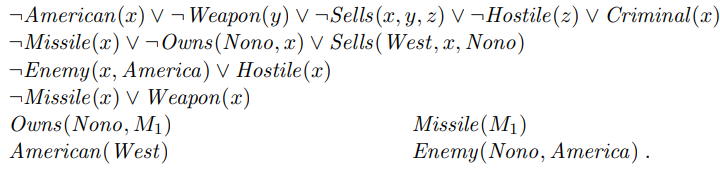
\includegraphics[]{images/crime-cnf.png}
    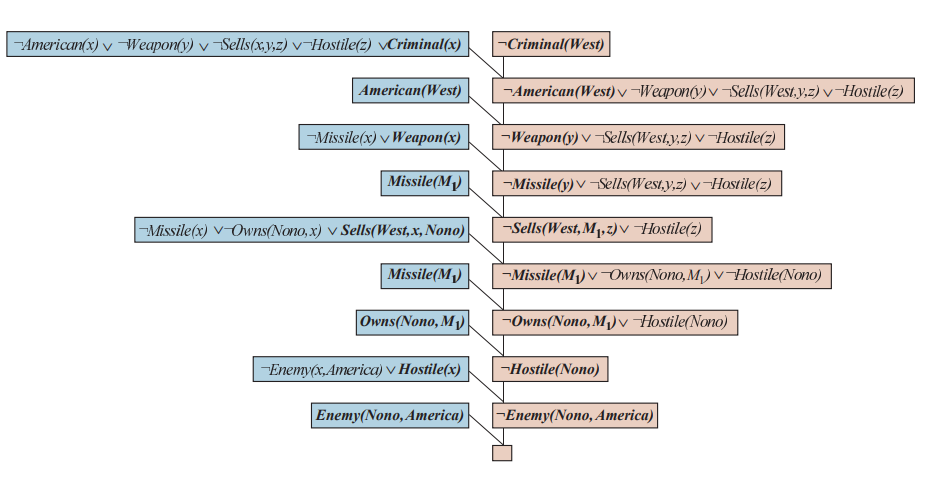
\includegraphics[]{images/resolution-crime-fol.png}
\end{center}
The resolution proof is shown in the figure above. Notice the structure: single “spine” beginning with the goal clause, resolving against clauses from the knowledge base until the empty clause is generated. This is characteristic
of resolution on Horn clause knowledge bases. In fact, the clauses along the main spine correspond exactly to the consecutive values of the goals variable in the backward-chaining algorithm.\\\\
Our second example makes use of Skolemization and involves clauses that are not definite clauses. This results in a somewhat more complex proof structure. In English, the problem is as follows:
\begin{center}
    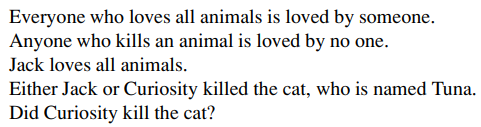
\includegraphics[]{images/resolution-fol-proof.png}
\end{center}
First, we express the original sentences, some background knowledge, and the negated goal G in first-order logic:
\begin{center}
    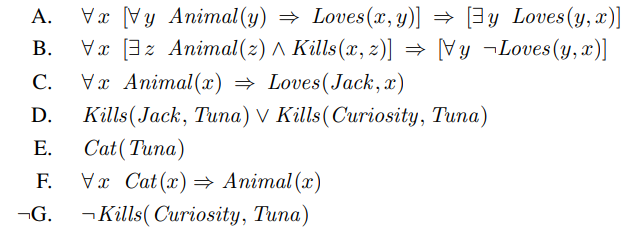
\includegraphics[]{images/kb-res-proof.png}
\end{center}
Now we apply the conversion procedure to convert each sentence to CNF:
\begin{center}
    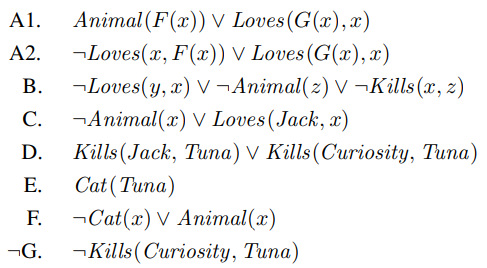
\includegraphics[]{images/kb-cnf-re-prrof.png}
\end{center}
The resolution proof that Curiosity killed the cat is given in the figure below:
\begin{center}
    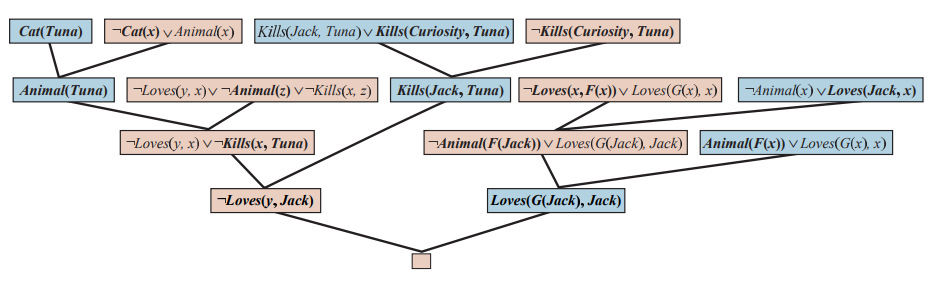
\includegraphics[]{images/res-proof-tree.png}
\end{center}
The proof answers the question “Did Curiosity kill the cat?” but often we want to pose more general questions, such as “Who killed the cat?”. Then, the goal is $\exists w \, Kills(w, Tuna)$, which, when negated, becomes $\neg Kills(w, Tuna)$ in CNF. Repeating the proof with the new negated goal, we obtain a similar proof tree, but with the substitution {w/Curiosity} in one of the steps. Unfortunately, resolution can produce \textbf{nonconstructive proofs} for existential goals. For example, $\neg Kills(w, Tuna)$ resolves with $Kills(Jack, Tuna) \lor Kills(Curiosity, Tuna)$ to give $Kills(Jack, Tuna)$, which resolves again with $\neg Kills(w, Tuna)$ to yield the empty clause. Notice that $w$ has two different bindings in this proof; resolution is telling us that, yes, someone killed Tuna, either Jack or Curiosity. This is no great surprise!
\begin{center}
    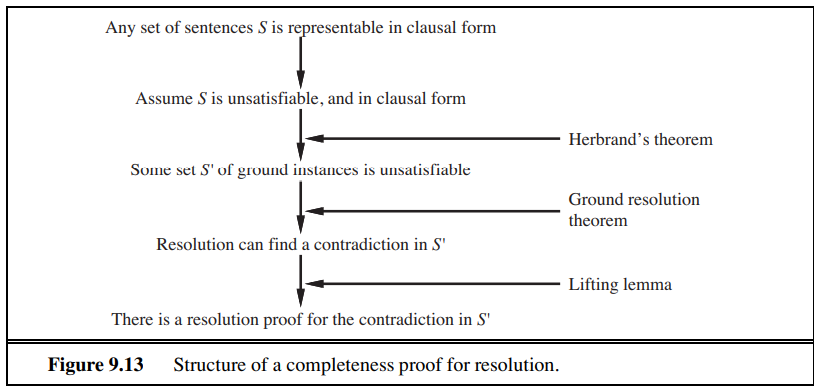
\includegraphics[]{images/res-completeness-fol.png}
\end{center}

\section{Resolution strategies}
We know that repeated applications of the resolution inference rule will eventually find a proof if one exists. In this subsection, we examine strategies that help find proofs efficiently.
\begin{itemize}
    \item \textbf{Unit preference/clause}: prefers to do resolutions where one of the sentences is a single literal.  The idea behind the strategy is that we are trying to produce an empty clause, so it might be a good idea to prefer inferences that produce shorter clauses.

    \item \textbf{Unit resolution:} is a restricted form of resolution in which every resolution step \textbf{must} involve a unit clause. Unit resolution is incomplete in general, but complete for Horn clauses. Unit resolution proofs on Horn clauses resemble forward chaining.

    \item \textbf{Set of support:} every resolution step involve at least one element of a special set of clauses (the set of support); the resolvent is then added into the set of support. Incomplete if the wrong set of support is chosen.

    \item \textbf{Input resolution:} In this strategy, every resolution combines one of the input sentences (from the KB or the query) with some other sentence. Complete for knowledge bases that are in Horn form, but incomplete in the general case. Input resolution has the characteristic shape of a single “spine” with single sentences combining onto the spine. The \textbf{linear resolution} strategy is a slight generalization that allows $P$ and $Q$ to be resolved together either if $P$ is in the original KB or if $P$ is an ancestor of $Q$ in the proof tree. Linear resolution is complete.

    \item \textbf{Subsumption:} eliminates all sentences that are subsumed by (that is, more specific than) an existing sentence in the KB. For example, if $P(x)$ is in the KB, then there is no sense in adding $P(A)$ and even less sense in adding $P(A) \lor Q(B)$. Subsumption helps keep the KB small and thus helps keep the search space small.

\end{itemize}

\chapter{Lec 14 - Higher-order functions for trees III}

\section{Trees type definition}
Until now we used binary trees that support data only in the leaves. Let's change the type definition in order to support information attached to nodes. We can do this in many different ways:
\begin{lstlisting}[style = FSharpStyle]
    type 'a tree =
        | Node of 'a * 'a tree * 'a tree
        | Leaf of 'a
\end{lstlisting}
In this case, a node is composed by an element of type 'a (which is the information attached to it) and the two sub-trees. However, with this definition we wouldn't be able to represent dead branches. In fact, each node must always have two sub-trees that can be either another node or a leaf.
\begin{lstlisting}[style = FSharpStyle]
    type 'a tree =
        | Node of 'a * 'a tree * 'a tree
        | Leaf of 'a option
\end{lstlisting}
With this implementation we can represent a dead branch defining a Leaf of None, but we could even define nodes with two empty leaves. So, this definition allows the programmer to write things that are not in their most simplified form.\newline\newline
In order to prevent this, we can do the following:
\begin{lstlisting}[style = FSharpStyle]
    type 'a tree =
        | Node of 'a * 'a tree option * 'a tree option
\end{lstlisting}
Now the \textbf{Node} data-constructor is a triple composed by:
\begin{itemize}
    \item An element of type 'a (information in the node)
    \item Two 'a tree option elements which represent the left and right sub-trees
\end{itemize}
When both the sub-trees are None, we are representing a leaf.\newline\newline
Let's write in F\# the following tree using this definition:\newline
\begin{tikzpicture}
    \Tree
    [.5  
        [.6
            \edge[]; {1}
            \edge[]; {2}
        ]
        [.7
            \edge[]; {3}
            \edge[blank]; \node[blank]{};
        ]
    ]
\end{tikzpicture}\newline
\begin{lstlisting}[style = FSharpStyle]
    let Leaf x = Some(Node(x, None, None))
    let tree = Node(5,
                Some(Node(6, Leaf 1, Leaf 2)),
                Some(Node(7, Leaf 3, None)))
\end{lstlisting}
Note that \textbf{Leaf x} is a function, not a data-constructor. It is just a shorter way to define leaves. The difference between functions and data-constructors is that functions can be used to \textbf{create}, but not for deconstructing (they can't be used to pattern-match).\newline\newline
We can write trees even in a shorter form by defining the following function:
\begin{lstlisting}[style = FSharpStyle]
    let SNode (x, t1, t2) = Some (Node (x, t1, t2))
    let tree = Node (5, 
               SNode (6, Leaf 1, Leaf 2), 
               SNode (7, Leaf 3, None)
               )
\end{lstlisting}
How can we pattern-match this type definition ? We have to specify all possible combinations of node types.
\begin{lstlisting}[style = FSharpStyle]
    let rec pretty_tree t = 
        match t with
        | Node(x, None, None) -> sprintf "(. %O .)" x
        | Node(x, Some l, Some r) -> sprintf "(%s %O %s)" (pretty_tree l) x (pretty_tree r)
        | Node(x, Some l, None) -> sprintf "(%s %O %s)" (pretty_tree l) x "."
        | Node (x, None, Some r) -> sprintf "(%s %O %s)" "." x (pretty_tree r)
        
    let st = pretty_tree tree

    // val st : string = "(((. 1 .) 6 (. 2 .)) 5 ((. 3 .) 7 .))"
\end{lstlisting}
The function above is a \textbf{pretty\_print} function for trees, which is a function that produces a string that represents the given tree. Instead of specify all the possibilities in the pattern-match, we can simplify things by defining an additional function. 
\begin{lstlisting}[style = FSharpStyle]
    let pretty_opt f o = 
        match o with 
        | None -> "."
        | Some x -> f x

    let rec pretty_tree t =
        match t with
        | Node (x, lo, ro) -> 
            let l = pretty_opt pretty_tree lo
            let r = pretty_opt pretty_tree ro
            sprintf "(%s %O %s)"  l x r
    
    let st = pretty_tree tree

    // val st : string = "(((. 1 .) 6 (. 2 .)) 5 ((. 3 .) 7 .))"
\end{lstlisting}
\section{Record types}
In F\# we can define the so called \textbf{record types} using the following syntax:
\begin{lstlisting}[style = FSharpStyle]
    type 'a tree = {data : 'a;
                     left : 'a tree option;
                     right : 'a tree option}
\end{lstlisting}
Records are series of \textit{Label : type} separated by a semicolon.


\chapter{Lec 15 - Sequence Modeling}

\section{Learning in Sequential Domains}
Why learning in sequential domains is different than static domains ? Because successive points in sequential data are \textbf{strongly correlated}. Machine learning models and algorithms for sequence learning have to consider that data points are not independent, deal with sequential distortions and/or variations (e.g. In speech, variations in speaking rate) and make use of \textbf{contextual information}.
\newline\newline
With static data we usually learn:
\[P(\textbf{o}|\textbf{x})\]
where $\textbf{x}$ is a fixed-size tuple of predictive attributes and $\textbf{o}$ is a classification/regression task.\newline\newline
With \textbf{sequential data}, instead, $\textbf{x}$ is a \textbf{sequence} $x^{(1)}, ..., x^{(t)}, ...$ where each $x^{(t)}$ has a static type. $\textbf{o}$ may be either static (e.g., sequence classification) or a sequence.\newline\newline
Using mathematical induction, a \textbf{sequence} is either an external vertex, or an ordered pair $(t, h)$ where the head $h$ is a vertex and the tail $t$ is a sequence.

\subsection{Sequencial Transductions}
Sequence Transduction is a machine learning task that involves converting an input sequence into an output sequence, potentially of different lengths.\newline\newline
Let $X$ and $O$ be the \textbf{input} and \textbf{output} label spaces. We denote by $X^*$ the set of all sequences with labels in $X$. We can define a general transduction $T$ as a function
\[T : X^* \rightarrow O^*\]
\begin{itemize}
    \item $T(\cdot)$ has \textbf{finite memory} $k \in \mathbb{N}$ if $\forall \textbf{x} \in X^*$ and $\forall t$, $T(x^{(t)})$ only depends on $\{\textbf{x}^{(t)}, \textbf{x}^{(t-1)}, ..., \textbf{x}^{(t-k)}\}$ 

    \item $T(\cdot)$ is \textbf{algebraic} if it has 0 finite memory (i.e., no memory at all)

    \item A transduction $T(\cdot)$ is \textbf{causal} if the output at time $t$ does not depend on future inputs (at time $t + 1, t + 2,...$ )

\end{itemize}

\subsection{Learning Sequences}
Sequences have variable length but typical machine learning models
have a fixed number of inputs. In order to solve this problem we can:
\begin{itemize}
    \item Limit context to a \textbf{fixed-size window}.
    \item Use \textbf{recurrent} models.
    \item Use \textbf{transformers} for non-causal sequences (e.g. text).
\end{itemize}


\section{Recursive State Representation}
In order to represent a recursive state we can use the following equations:
\[\begin{split}
    h^{(t)} & = f(h^{(t-1)}, x^{(t)}, t)\\
    o^{(t)} & = g(h^{(t)}, x^{(t)}, t)
\end{split}\]
where $f$ is the \textit{state transition function} and $g$ is the \textit{output function}. 
\newline\newline
$h^{(t)}$ is called the state of the system and it's defined by a \textbf{recursive equation}. Indeed, the definition of $h$ at time $t$ refers back to the same definition at time $t - 1$. It contains information about the whole past sequence. For a finite number of time steps $\tau$, the graph can be unfolded by applying the definition $\tau - 1$ times. \textbf{Unfolding} the equation by repeatedly applying the definition yields an expression that does not involve recurrence. Such an expression can now be represented by a traditional directed acyclic computational graph.
\begin{center}
    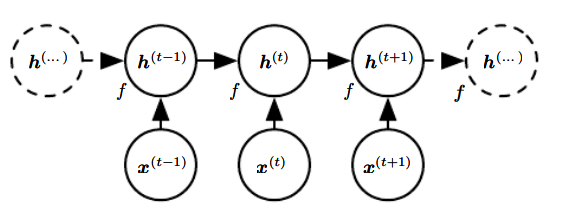
\includegraphics[]{images/recurrent-graph.png}
\end{center}
The state transition function can be represented using the time shift operator $q^{-1}$:
\[q^{-1}h^{(t)} = h^{(t-1)}\]
\begin{center}
    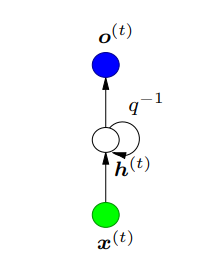
\includegraphics[]{images/time-shift-op.png}
\end{center}
The unfolding process thus introduces two major advantages:
\begin{enumerate}
    \item Regardless of the sequence length, the learned model always has the same input size, because it is specified in terms of transition from one state to another state, rather than specified in terms of a variable-length history of states.

    \item It is possible to use the same transition function $f$ with the same parameters at every time step.
\end{enumerate}
These two factors make it possible to learn a single model that operates on all time steps and all sequence lengths. Learning a single, shared model allows generalization to sequence lengths that did not appear in the training set, and allows the model to be estimated with far fewer training examples than would be required without parameter sharing.\newline\newline
Given a sequence $s \in X^{*}$ and a recursive transduction $T$, the \textit{encoding network} associated to $s$ and $T$ is formed by unrolling (time unfolding) the recursive network of $T$ through the input sequence $s$.
\begin{center}
    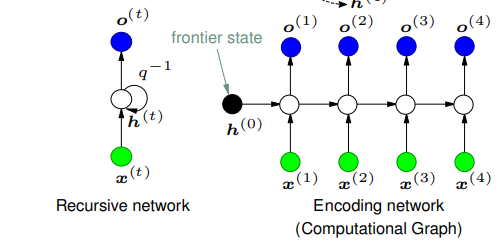
\includegraphics[]{images/encoding-network.png}
    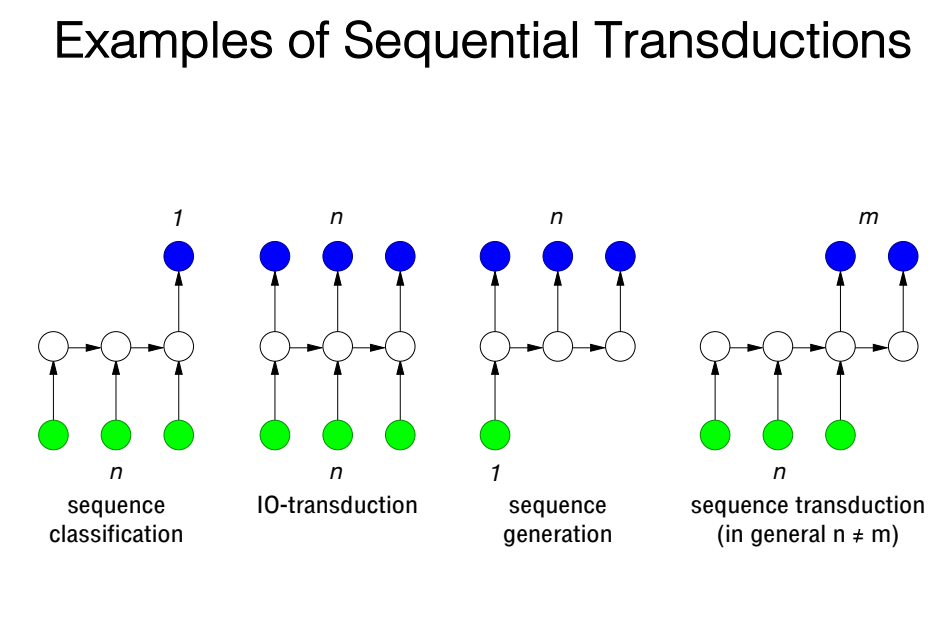
\includegraphics[scale=0.7]{images/sequential--transduction.png}
\end{center}
$T$ is \textbf{stationary} if $f(\cdot)$ and $g(\cdot)$ do not depend on $t$\newline\newline
There are different ways in which we can implement $f(\cdot)$ and $g(\cdot)$. There are two general families of models:
\begin{itemize}
    \item Linear:
    \begin{itemize}
        \item Kalman Filter
        \item Hidden Markov Models
        \item Linear Dynamical Systems
        \item ...
    \end{itemize}
    \item Nonlinear
    \begin{itemize}
        \item Recurrent Neural Networks
        \item ...
    \end{itemize}
\end{itemize}

\section{Shallow Recurrent Neural Networks}
Armed with the graph unrolling and parameter sharing ideas, we can design a wide variety of recurrent neural networks. In general we have:
\[\begin{split}
    \textbf{h}^{(t)} & = f(\textbf{U}\textbf{x}^{(t)} + \textbf{W}\textbf{h}^{(t-1)} + \textbf{b})\\
    \textbf{o}^{(t)} & = g(\textbf{V}\textbf{h}^{(t)} + \textbf{c})
\end{split}\]
where $f()$ and $g()$ are non-linear functions (e.g. $tanh()$ and $softmax$), and $h^{(0)} = 0$ (or can be learned jointly with the other parameters). $\textbf{U}$ and $\textbf{W}$ are weight matrices which parametrize \textbf{input-to-hidden} connections and \textbf{hidden-to-hidden} recurrent connections respectively. \textbf{Hidden-to-output} connections are parametrized by the weight matrix $\textbf{V}$.\newline\newline
An example of RNN for IO-transduction with discrete outputs:
\[\begin{split}
    \textbf{h}^{(t)} & = tanh(\textbf{U}\textbf{x}^{(t)} + \textbf{W}\textbf{h}^{(t-1)} + \textbf{b})\\
    \textbf{o}^{(t)} & = \textbf{V}\textbf{h}^{(t)} + \textbf{c}\\
    \hat{\textbf{y}} & = softmax(\textbf{o}^{(t)})\\
    L & = \sum_t L^{(t)} = - \sum_t log\,p_{model}(\textbf{y}^{(t)} | \{\textbf{x}^{1}, ..., \textbf{x}^{(t)}\})
\end{split}\]
where:
\begin{itemize}
    \item $o^{(t)}$ is the unnormalized log probabilities a time $t$
    \item $\textbf{y}^{(t)}$ is the target vector a time $t$
    \item $p_{model}(\textbf{y}^{(t)} | \{\textbf{x}^{1}, ..., \textbf{x}^{(t)}\}$ is given by reading the entry for $\textbf{y}^{(t)}$ from the model’s output vector $\hat{\textbf{y}}^{(t)}$, that is, the loss $L$ \textbf{internally computes} $\hat{\textbf{y}}$.
    \item $L$ is the loss function
\end{itemize}
The corresponding computation graph is the following
\begin{center}
    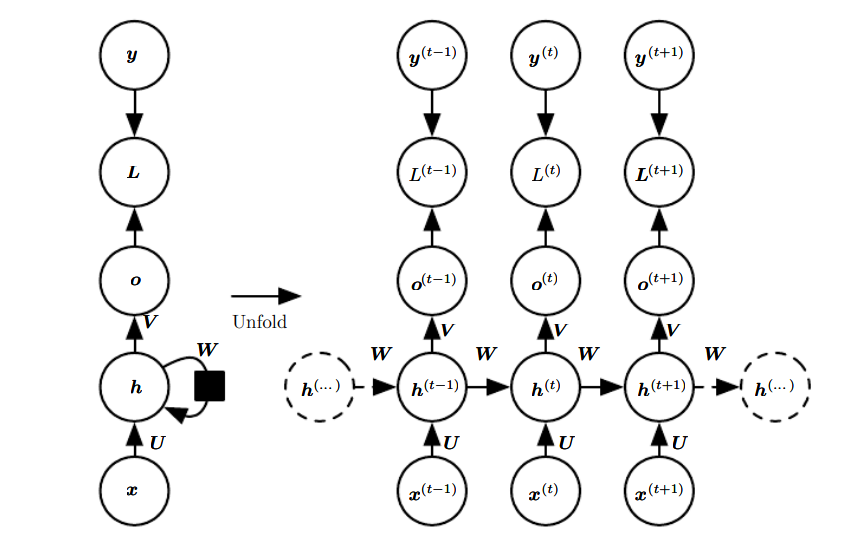
\includegraphics[scale=0.8]{images/rnn-computational-graph.png}
\end{center}
Some examples of important design patterns for recurrent neural networks
include the following:
\begin{itemize}
    \item Recurrent networks that produce an output at each time step and have recurrent connections between hidden units (IO-transduction).

    \item Recurrent networks that produce an output at each time step and have recurrent connections only from the output at one time step to the hidden units at the next time step

    \item Recurrent networks with recurrent connections between hidden units, that read an entire sequence and then produce a single output (e.g. for classification).
\end{itemize}
There are a lot of possible additional architectural features, such as short-cut connections, higher-order states, feedback from output, teacher forcing, bidirectional RNN, etc\footnote{See slides for further information}. All these architectural features (and others...) are orthogonal, i.e. they can be combined together.


\subsection{Teacher Forcing}
The network with recurrent connections only from the output at one time step to the hidden units at the next time step is strictly less powerful because it lacks hidden-to-hidden recurrent connections. Therefore, it requires that the output units capture all of the information about the past that the network will use to predict the future. Because the output units are explicitly trained to match the training set targets, they are unlikely to capture the necessary information about the past history of the input.\newline\newline
For this reason, models that have recurrent connections from their outputs leading back into the model may be trained with \textbf{teacher forcing}. Teacher forcing is a procedure in which during training the model receives the ground truth output $\textbf{y}^{(t)}$ as input at time $t + 1$. When the model is deployed, the true output is generally not known. In this case, we approximate the correct output $\textbf{y}^{(t)}$ with the model’s output $\textbf{o}^{(t)}$, and feed the output back into the model.
\[\begin{split}
    \textbf{h}^{(t)} & = tanh(\textbf{U}\textbf{x}^{(t)} + \textbf{W}\textbf{y}^{(t-1)} + \textbf{b})\\
    \textbf{o}^{(t)} & = \textbf{V}\textbf{h}^{(t)} + \textbf{c}\\
    \hat{\textbf{y}} & = softmax(\textbf{o}^{(t)})\\
    L & = - \sum_t log\,p_{model}(\textbf{y}^{(t)} | \textbf{y}^{(1)}, ..., \textbf{y}^{(t-1)}, \textbf{x}^{(1)}, ..., \textbf{x}^{(t)})
\end{split}\]
\begin{center}
    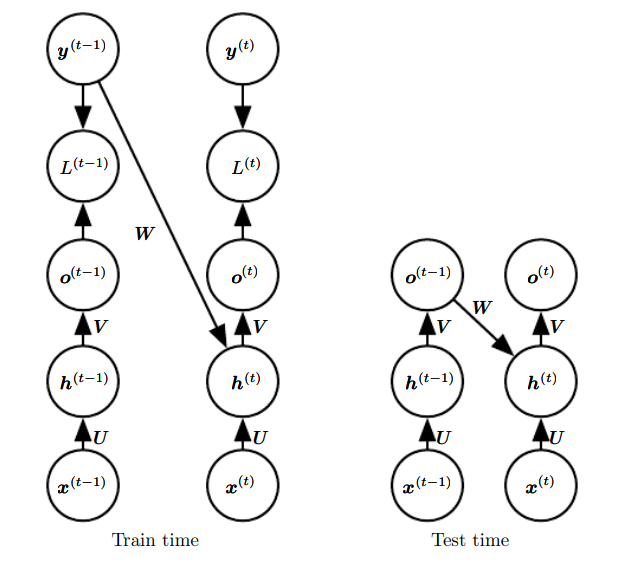
\includegraphics[]{images/teacher-forcing.png}
\end{center}
The advantage of eliminating hidden-to-hidden recurrence is that, for any loss function based on comparing the prediction at time $t$ to the training target at time $t$, all the time steps are decoupled. Training can thus be parallelized, with the gradient for each step $t$ computed in isolation.

\subsection{Bidirectional RNNs}
in many applications we want to output a prediction of $\textbf{y}^{(t)}$ which may depend on the whole input sequence. For example, if there
are two interpretations of the current word that are both plausible, we may have to look far into the future (and the past) to disambiguate them. Bidirectional recurrent neural networks (or bidirectional RNNs) were invented to address that need.\newline\newline
As the name suggests, bidirectional RNNs combine an RNN that moves forward
through time, beginning from the start of the sequence, with another RNN that moves backward through time, beginning from the end of the sequence.
\begin{center}
    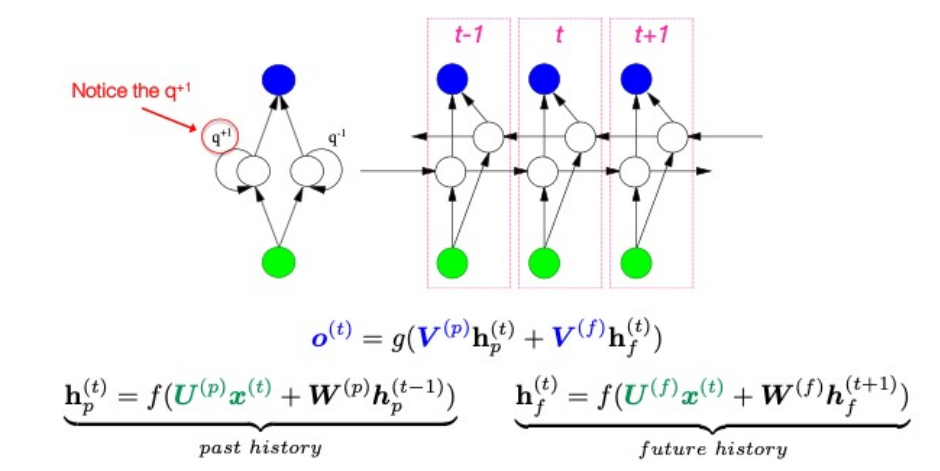
\includegraphics[scale=0.9]{images/bidirectional-rnn.png}
\end{center}

\subsection{1 to \textit{n} transduction}
Previously, we have discussed RNNs that take a sequence of vectors $\textbf{x}^{(t)}$ for $t = 1, ..., \tau$ as input. Another option is to take only a single vector $\textbf{x}$ as input. When $\textbf{x}$ is a fixed-size vector, we can simply make it an extra input of the RNN
that generates the $\textbf{y}$ sequence.  The interaction between the input $\textbf{x}$ and each hidden unit vector $\textbf{h}^{(t)}$ is parametrized by a newly introduced weight matrix $\textbf{R}$.
\begin{center}
    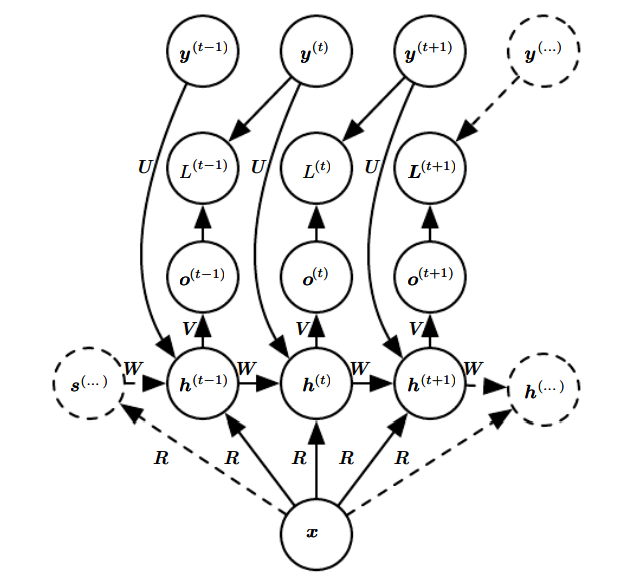
\includegraphics[scale=0.8]{images/1-to-n transduction.png}
\end{center}
Each element $\textbf{y}^{(t)}$ of the observed output sequence serves both as input (for the current hidden unit at time $t$) and, during training, as target (for the previous output unit at time $t-1$).\newline\newline
This RNN is appropriate for tasks such as image captioning, where a single image is used as input to a model that then produces a sequence of words describing the image.

\subsection{Encoder-Decoder Sequence-to-Sequence Architectures}
Here we discuss how an RNN can be trained to map an input sequence to an output sequence which is not necessarily of the same length. This comes up in many applications, such as speech recognition, machine translation, etc.\newline\newline
An encoder-decoder RNN architecture is is composed of an encoder RNN that reads the input sequence and a decoder RNN that generates the output sequence. The final hidden state of the encoder RNN is used to compute a generally fixed-size context variable $C$ which represents a semantic summary of the input sequence and is given as input to the decoder RNN.
\begin{center}
    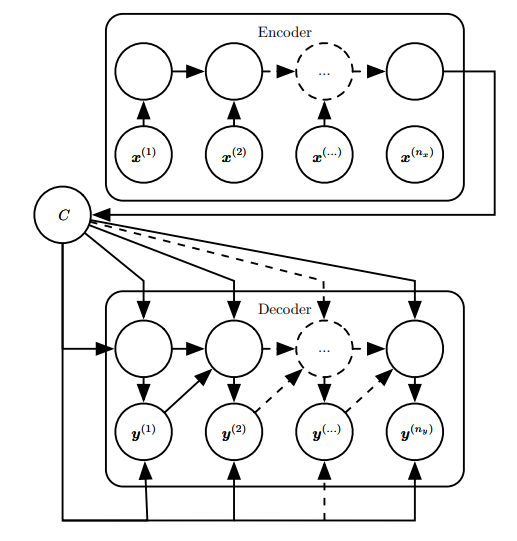
\includegraphics[]{images/encoder-decoder rnn.png}
\end{center}
If the context $C$ is a vector, then the decoder RNN is simply a vector-to-sequence RNN.


\chapter{Lec 16 - Graph Neural Networks}

\section{Introduction}
Traditional ML approaches have been developed assuming data to be encoded into feature vectors; however, many important real-world applications generate data that are naturally represented by more complex structures, such as graphs. Graphs are particularly suited to
represent the relations (arcs) between the components (nodes) constituting an entity. For instance, in social network data, single data “points” (i.e., users) are closely inter-related.\newline\newline
A graph $G = (V, E)$ can be represented using the so called \textbf{adjacency matrix}. A $n \times n$ matrix $A$ such that $A[i,j] = 1$ if $edge(i,j) \in E$, 0 otherwise.\newline\newline
    \textbf{Example:}\newline\newline
    \begin{center}
        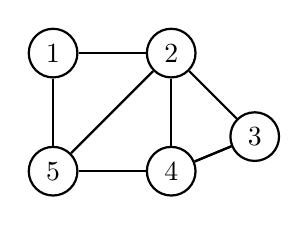
\begin{tikzpicture}[node distance={15mm}, thick, main/.style = {draw, circle}] 
            \node[main] (1) {$1$}; 
            \node[main] (2) [right of=1] {$2$}; 
            \node[main] (3) [below right of=2] {$3$}; 
            \node[main] (4) [below of=2] {$4$}; 
            \node[main] (5) [below of=1] {$5$}; 
            \draw (1) -- (2); 
            \draw (1) -- (5); 
            \draw (2) -- (5);
            \draw (2) -- (4);
            \draw (5) -- (4);
            \draw (3) -- (4); 
            \draw (5) -- (4);
            \draw (4) -- (3);
            \draw (2) -- (3);
        \end{tikzpicture}
    \end{center}
    The Adjacency matrix of the graph above is the following:
    \[\begin{bmatrix}
        0 & 1 & 0 & 0 & 1 \\
        1 & 0 & 1 & 1 & 1 \\
        0 & 1 & 0 & 1 & 0 \\
        0 & 1 & 1 & 0 & 1 \\
        1 & 1 & 0 & 1 & 0
    \end{bmatrix}\]
In undirected graphs this matrix is \textbf{symmetric}, while in directed graphs it is \textbf{asymmetric}. In case of a weighted graph, each cell of the matrix has either the value of the edge weight $w$ or $-$. Each node and edge is represented by a feature vector:
\begin{center}
    \includegraphics[scale=0.5]{images/graphs.png}
\end{center}
The position $(m,n)$, of the adjacency matrix contains the number of walks of length one from node $m$ to node $n$. Position $(m,n)$ of the \textbf{squared} adjacency matrix $A^2$ contains the number of walks of length two from node $m$ to node $n$.\newline\newline
The main problem settings that can arise when dealing with structured data are the following:
\begin{itemize}
    \item Predictions over \textbf{nodes} in a network: In this setting, the dataset is composed of a single (possibly disconnected) large graph. Each example is a node in the graph, and the learning tasks are defined as predictions over the nodes. Given an unseen node $u$, the task is to predict the correct target $y_u$. An example in this setting is the prediction of properties of a social network user based on his or her connections.

    \item Predictions over \textbf{graphs}: In this case, each example is composed of a whole graph, and the learning tasks are predictions of properties of the whole graphs. An example is the prediction of toxicity in humans of chemical compounds represented by their molecular graph.

    \item Link-prediction tasks: the model predicts whether or not there should be an edge between nodes. 
\end{itemize}

\section{Learning on graphs is difficult}
Let $\textbf{X}$ be the matrix in which the feature vectors of each node are stored. We can observe that node indexing in graphs is arbitrary. This means that, differently from images, permuting the node indices results in a permutation of the columns of $\textbf{X}$ and a permutation of both the rows and columns of $A$. However, the underlying graph is unchanged. This property is called Permutation Invariance. More formally, given a permutation matrix $\textbf{P}$, we get a different representation of the same graph:
\[\begin{split}
    \textbf{X}' & = \textbf{XP}\\
    \textbf{A}' & = \textbf{P}^T \textbf{AP}
\end{split}
\]
This property can give the intuition about why learning on graphs is difficult. In fact, determining if two graphs are equal (graphs isomorphism) is a problem for which are not known polynomial-time algorithms. Furthermore, sub-graph isomorphism, which is the problem of determining if a graph is a sub-graph of another graph, is NP-Complete. These problems affect machine learning because a model should be able to predict the same output for isomorphic graphs (which can be represented in different ways). Furthermore, the model we design should capture the similarity between two graphs (sub-graph isomorphism).\newline\newline
In general, the main problems we face when learning on graphs are the following:
\begin{enumerate}
    \item Same graph can be represented in different ways;
    \item How to recognize that a given graph $G_2$ is a sub-graph of $G_1$
    \item How to represent graphs of different sizes (i.e., different number of nodes) into fixed-size vectors without loosing expressiveness ?

    \item How to avoid explosion in the number of parameters with the size of the graphs?
    
\end{enumerate}
Problem 3 is commonly faced by using recursive models that exploit a
causal state space [Sperduti \& Starita., TNN 1997], while Problem 4  is commonly faced by exploiting shared parameters.\newline\newline
Regarding Problems 1 and 2, a sound and meaningful representation for graphs can be achieved by using a neural network with \textbf{convolution operator}, defined on graphs.

\section{Graph Neural Networks - General Idea}
A Graph Neural Network (GNN) receives in input a graph (adj. matrix and node representations. for simplicity) and passes it through a series of $k$ layers. Each layer computes a hidden representation for each node, with the last layer computing the final nodes' embeddings $\textbf{H}_k$. Similarly to CNNs, each node representation includes information about the node and its context within the graph.
\begin{itemize}
    \item For \textbf{node-level tasks}, the output is computed from $\textbf{H}_k$;

    \item For \textbf{graph-level tasks}, the nodes' embeddings are combined (e.g., by averaging), and the resulting vector is mapped via a linear transformation or neural network to a fixed-size vector from which the classification/regression task is performed.

    \item For \textbf{link-prediction tasks}, the embeddings of the two endpoint nodes must be mapped to a single number representing the probability that the edge is present (e.g. dot product of the nodes' embeddings and pass the result through a sigmoid function to create a probability).
 
\end{itemize}
\begin{center}
    \includegraphics[]{images/gnn.png}
\end{center}

\section{Graph Convolution}
The general idea of graph convolution starts from a parallel between graphs and images. GNNs implement convolution in a similar way how CNNs do, that is, learning the features by inspecting neighboring nodes. GNNs generalize the definition of convolution for non-regular structured data.

\subsection{NN4G by Micheli}
\textbf{NN4G} is an architecture based on a graph convolution that is defined as:
\begin{center}
    \includegraphics[scale=0.6]{images/nn4g.png}
\end{center}
where: 
\begin{itemize}
    \item $\sigma$ is a nonlinear activation function applied element-wise.
    \item $N(v)$ represent the neighborhood of node $v$.
    \item $\textbf{W}^i$ is a weights' matrix;
    \item $\textbf{x}_u$ is the feature vector of node $u$.
\end{itemize}
Actually, this is a simplified notation, since the original one uses skip connections (see GNN book chapter).
\begin{center}
    \includegraphics[]{images/nn4g-2.png}
\end{center}
Note that:
\begin{itemize}
    \item The first layer ($i = 1$), which has no previous layers, computes the nodes' representations only on the basis of each vertex feature vector.

    \item Each convolution performed on the $i$-th hidden units, with $i > 1$, takes as input the neighbors' representations of the previous layer. Basically, it merges the representations of each node with those of its neighbors:

    \item $X_1(g), X_2(g), X_3(g)$ are scalar values computed by aggregating the representations $\textbf{x}_i(g)$ for each unit $i$.
    In particular they are defined as:
    \[X_i(g) = \frac{1}{k}\sum_{v \in Vert(g)}x_i(v)\]
    if $k = 1$, this corresponds to a sum. Basically, we compute a representation per-graph per-layer. Then, this 3 representations are parametrized by the weights $w_1, w_2, w_3$ and used to compute the output for the whole graph (graph-level task).
\end{itemize}
The convolutional operation presented above can be defined in a compact way using matrix multiplications:
\begin{center}
    \includegraphics[scale=0.6]{images/matrix-gcn.png}
\end{center}
where $\textbf{A}$ is the adjacency matrix. Exploiting matrix multiplications makes the computation really fast. Furthermore, note that, as for images, the receptive field of the layers increases as we stack more layers.\newline\newline
Note also that, since with the convolution operator we are merging neighboring nodes' representations, isomorphic graphs in which the order of the nodes is changed will have the same nodes' representations.

\subsection{Graph Fourier Transform}
The operation described above is graph convolution, but how it is derived? Defining the formal convolution operator on graph is difficult.\newline\newline
Let $x: V \rightarrow \mathbb{R}$ be a signal on the nodes $V$ of the graph $G$, i.e., a function that associates a real value with each node of $V$. We can represent every signal as a vector $\textbf{x} \in \mathbb{R}^n$, which from now on we will refer to as signal. In order to set up a convolutional network on $G$, we need the notion of convolution between a signal $\textbf{x}$ and a filter signal $\textbf{f}$.\newline\newline
The key idea is to use a Fourier transform. In the frequency domain, thanks to the \textbf{Convolution Theorem}, the (undefined) convolution of two signals becomes the (well-defined) component-wise product of their transforms. So, if we knew how to compute the Fourier transform of a function defined on a graph, we could define the convolution operator.\newline\newline
The Convolution Theorem states that convolution in one domain (time, space) corresponds to pointwise multiplication in frequency domain.\newline\newline
The \textbf{graph Fourier transform} is defined starting from the (normalized) Laplacian matrix of the graph, which is defined as:
\[L = I_n - D^{-\frac{1}{2}} A D^{-\frac{1}{2}}\]
where:
\begin{itemize}
    \item $I_n$ is the identity matrix;
    \item $A$ is the adjacency matrix;
    \item $D$ is the degree matrix, that is, the \textbf{diagonal} matrix containing the number of edges attached to each vertex;
\end{itemize}
Then, we can compute the eigendecomposition of $L$ (which is always possible):
\[L = U \Lambda U^T\]
where $\Lambda = diag([\lambda_0, ..., \lambda_{n-1}])$ and $U$ is the Fourier basis of the graph.\newline\newline
Finally, Given a spatial signal $\textbf{x}$:
\begin{itemize}
    \item $\hat{\textbf{x}} = U^T\textbf{x}$ is its graph Fourier Transform

    \item $\textbf{x} = U \hat{\textbf{x}}$ is the inverse Fourier transform
\end{itemize}
Therefore, convolution between a parametric filter and a signal can be defined as:
\[y = \textbf{f}_\theta *_G \textbf{x} = U\left( (U^T\textbf{f}_\theta) \odot (U^T \textbf{x})\right)\]
It can be proved that this operator corresponds to the one used for NN4G presented previously (see slides for more details).

\section{Aggregation Layer for graph classification}
With Graph Convolution we have a representation for each graph node. How can we map node representations to a graph-level representation? There are some simple solutions, like the sum or the average of nodes' representations as we saw previously, or we can rely on more complex alternatives: Universal readout.


\section{Graph Recurrent Neural Networks}
Scarselli et al. proposed a network architecture where, instead of stacking multiple layers, a single recurrent layer is adopted:
\[\textbf{h}_v^{t+1} = \sum_{u \in N(v)}f(\textbf{h}_u^t, \textbf{x}_v, \textbf{x}_u)\]
where $f$ is a function (e.g. neural network) with shared parameters across all the nodes and all the time steps. The recurrent system is defined as a contraction mapping, and thus it is guaranteed to converge to a fixed point $\textbf{h*}$.

\subsection{Gated Graph Neural Networks}
The idea is to remove the constraint for the recurrent system to be a contraction mapping, and implement this idea by adopting recurrent
neural networks to define the recurrence. Specifically, the gated recurrent unit (GRU) is adopted. The recurrent convolution operator is defined as follows:
\begin{center}
    \includegraphics[scale=0.8]{images/gated-gnn.png}
\end{center}
where $\textbf{A}_v$ is row $v$ of the adjacency matrix $\textbf{A}$.


\chapter{Back-Propagation Through Time}

\section{BPTT}
\begin{figure}
    \centering
    \includegraphics[scale=0.2]{images/bptt_1.PNG}
    \label{fig:enter-label}
\end{figure}
\begin{figure}
    \centering
    \includegraphics[scale=0.2]{images/bptt_2.jpg}
    \label{fig:enter-label}
\end{figure}
\begin{figure}
    \centering
    \includegraphics[scale=0.3]{images/bptt_3.jpg}
    \label{fig:enter-label}
\end{figure}
\begin{figure}
    \centering
    \includegraphics[scale=0.3]{images/bptt4.jpg}
    \label{fig:enter-label}
\end{figure}
\chapter{Lec 18 - Long-Term Dependencies}

\section{Learning Long-Term Dependencies}
The basic problem of learning long-term dependencies is that gradients propagated over many stages tend to either vanish (most of the time) or explode\footnote{a problem when large error gradients accumulate and result in very large updates to neural network model weights during training} (rarely, but with much damage to the optimization).\newline\newline
A long-term dependency is when the desired output at time $t$ depends on the input at time $t - \tau$, with $t > \tau >> 1$ (e.g. $\textbf{x}^{(t - 100)} \rightarrow \textbf{y}^{(t)}$).\newline\newline
This means that, for the Recurrent Neural Network to output the correct
desired $\textbf{y}^{(t)}$, it has to recognize its dependency on $\textbf{x}^{(t - \tau)}$, and use $\textbf{x}^{(t - \tau)}$ in the generation of $\textbf{y}^{(t)}$.
\newline\newline
Here are some approaches to try to reduce the vanishing/exploding gradients
problem:
\begin{itemize}
    \item Architectural
    \begin{itemize}
        \item Long Short-Term Memory or Gated Recurrent units
        \item Reservoir Computing: Echo State Networks and Liquid State Machines
    \end{itemize}
    \item Algorithmic
    \begin{itemize}
        \item Clipping gradients (avoids exploding gradients)
        \item Hessian Free Optimization
        \item Smart Initialization: pre-training techniques
    \end{itemize}
\end{itemize}

\section{Long Short-Term Memory}
Long Short Term Memory networks - usually just called “LSTMs” - are a special kind of RNN, capable of learning long-term dependencies.\newline\newline
They are based on the idea of creating paths through time that have derivatives that neither vanish nor explode.\newline\newline
The mechanism allows the networks to “remember” relevant information for a long period of time and to "forget" them when they are no more relevant.
\newline\newline
The LSTM does have the ability to remove or add information to the cell state, carefully regulated by structures called gates. Gates are a way to optionally let information through. They are composed out of a sigmoid neural net layer and a pointwise multiplication operation. The sigmoid layer outputs numbers between zero and one, describing how much of each component should be let through. A value of zero means “let nothing through,” while a value of one means “let 
verything through!”
\newline\newline
An LSTM has three of these gates, to protect and control the cell state:
\begin{enumerate}
    \item Forget gate: The sigmoid layer called the “forget gate layer ”\textit{decides} what information we’re going to throw away from the cell state. It looks at $h^{(t-1)}$ and $x^{(t)}$, and outputs a number between 0 and 1 for each number in the cell state $C^{(t-1)}$ . A 1 represents “completely keep this” while a 0 represents “completely get rid of this.” Let $f_t$ be its output. The forget gate multiplies the old state by $f_t$, forgetting the things it decided to forget.
    \begin{center}
        \includegraphics[]{images/forget-gate.png}
    \end{center}

    \item Input gate: It decides what new information are going to be stored in the cell state. This has two parts. First, a sigmoid layer called the “input gate layer” decides which values are going to be updated. Let $i^t$ be its output. Next, a tanh layer creates a vector of new candidate values, $\Tilde{C^t}$, that could be added to the state. The input gate computes $i^t * \Tilde{C^t}$. The output of this gate is added to the output of the forget gate to determine the new cell state.
    \begin{center}
        \includegraphics[]{images/Input-gate.png}
        \includegraphics[scale=0.9]{images/new cell-state.png}
    \end{center}
    
    \item Output gate: It deterines what parts of the cell state are going to be outputted. It puts the cell state through tanh (to push the values to be between -1 and 1). The result is multiplied by the output of a sigmoid layer so that it only outputs the parts it decided to.
    \begin{center}
        \includegraphics[]{images/output-gate.png}
    \end{center}
\end{enumerate}
There are a lot of variations of the LSTM architecture. One popular variant is adding “peephole connections.” This means that we let the gate layers look at the cell state. Other variations are:
\begin{itemize}
    \item No Input Gate (NIG)
    \item No Forget Gate (NFG)
    \item No Output Gate (NOG)
    \item No Input Activation Function (NIAF)
    \item No Output Activation Function (NOAF)
\end{itemize}
However, vanilla LSTM performs reasonably well in general and variations do not significantly improve the performance. Furthermore, the forget gate is crucial for LSTM performance.

\section{Simplifying LSTM: Gated Recurrent Units}
The main difference between GRU and LSTM is that GRU uses a single gating unit that simultaneously controls the forgetting factor and the decision to update the state unit.
\begin{center}
    \includegraphics[]{images/GRU.png}
\end{center}
The update gate $\textbf{z}$ selects whether the hidden state need to be updated with a new hidden state $\Tilde{\textbf{h}}$. The reset gate $\textbf{r}$ decides whether the previous hidden state is ignored.\newline\newline
The values for $\textbf{z}$ and $\textbf{r}$ are defined as usual using the sigmoidal layers as in LSTM.\newline\newline
Basically, the idea is that if the $\textbf{z}$ vector has a value equal to 0 in position $i$, when we compute the element-wise multiplication between $\textbf{z}$ and $\textbf{h}^{(t-1)}$ the $i$-th value in $\textbf{h}^{(t-1)}$ will be cancelled. On the other hand, the $i$-th element in $(1 - \textbf{z})$ is 1. Therefore, the $i$-th element of $\textbf{h}^{(t-1)}$ will be updated with the $i$-th element of $\Tilde{\textbf{h}}$.

\section{Reservoir Computing}
Reservoir Computing is an umbrella term used to identify a general framework of computation derived from Recurrent Neural Networks (RNN). This technique can be implemented with \textbf{Echo State Networks} and \textbf{Liquid State Machines}. The idea is to fix the input-to-hidden and hidden-to-hidden connections at random values and only learn the output units connections. The intuition was born from the fact that in training RNNs most of the times the weights showing most change were the ones in the last layer.\newline\newline
The first part of the system, called Reservoir, is an RNN with fixed weights that acts as ”black-box” model of a complex system; The second one is known as Readout, a classifier layer of some kind, usually a simple linear one, connected by a set of weights to the Reservoir.\newline\newline
One way to think about these reservoir computing recurrent networks is that they are similar to kernel machines: they map an arbitrary length sequence (the history of inputs up to time $t$) into a fixed-length vector (the recurrent state $\textbf{h}^{(t)}$), on which a linear predictor (typically a linear regression) can be applied to solve
the problem of interest.\newline\newline
How do we set the input and recurrent weights so that a rich set of histories can be represented in the recurrent neural network state? in order to produce a “rich” set of dynamics, the reservoir should
\begin{itemize}
    \item be big (hundreds to thousands units).
    
    \item be sparsely (hidden weight matrix W up to 20\% possibile connections) and randomly (uniform distribution symmetric around zero) connected.

    \item satisfy the echo state property, i.e., the ability to forget information from the far past (or the effect of $\textbf{x}^{(t)}$ and $\textbf{h}^{(t)}$ on the future state should vanish gradually as time passes). This means that the spectral radius $\rho(\textbf{W}) < 1$, i.e, $\textbf{W}$ is contractive. 

    \item On the contrary, the input ($U$) and optional output feedback weight matrices are dense (still random with uniform distribution).
    
\end{itemize}
\textbf{Echo State Networks} are composed of standard standard recurrent neurons plus leaky integrators, while \textbf{Liquid State Machines} implements spiking integrate-and-fire neurons and dynamic synaptic connection models. A leaky integrator is defined as follows:
\[\textbf{h}^{(t)} = (1 - a)\textbf{h}^{(t-1)} + \sigma(\textbf{U} \textbf{x}^{(t)} + \textbf{W}\textbf{h}^{(t-1)})\]
Basically, it adds a portion of the previous state representation (according to $a$) to the new state representation.\newline\newline 
If the network is too contractive, it will forget too quickly information from the past. In order to overcome this problem we can use the \textbf{intrinsic plasticity} approach. The main idea is to exploit the full range of output of the activation function of the hidden units. IP is a computationally efficient online learning rule to adjust threshold and gain of sigmoid reservoir neurons. It drives the neurons’ output activities to approximate exponential distributions. The exponential distribution maximizes the entropy of a non-negative random variable with a fixed mean, thus enabling the neurons to transmit maximal information\newline\newline
To evaluate  a RC network we use memory capacity, which tells us if the internal state of the network can reproduce input from the far past :
\[\sum_{k=0}^\infty r^2 (\textbf{x}^{(t - k)}, \textbf{o}_k^{(t)})\]
where $r^2 (\textbf{x}^{(t - k)}, \textbf{o}_k^{(t)})$ is the squared correlation coefficient between the input $\textbf{x}^{(t - k)}$ with delay $k$ and the corresponding output $\textbf{o}_k^{(t)}$ generated by the network at time $t$ for delay $k$.

\section{Deep Recurrent Networks}
The computation in most RNNs can be decomposed into three blocks of parameters
and associated transformations:
\begin{enumerate}
    \item  from the input to the hidden state,
    \item  from the previous hidden state to the next hidden state, and
    \item  from the hidden state to the output.
\end{enumerate}
With the RNN architecture, each of these three blocks is associated with a single weight matrix. In other words, when the network is unfolded, each of these corresponds to a shallow transformation. By a shallow transformation, we mean a transformation that would be represented by a single layer within a deep MLP. Typically this is a transformation represented by a learned affine transformation followed by a fixed nonlinearity.\newline\newline
Experimental evidence shows a significant advantage if the state of an RNN is decomposed into multiple layers.  We can think of the lower layers in the hierarchy as playing a role in transforming the raw input into a representation that is more appropriate at the higher levels of the hidden state.\newline\newline
However, in general, it is easier to optimize shallow architectures and adding depth may hurt learning by making optimization difficult.


\chapter{Lec 19 - Reinforcement Learning}

\section{Reinforcement Learning}
An \textbf{Agent} operates in an environment $e$, which in response to action $a$ (given by the agent) in the state $s$ returns the next state and a reward $r$ (which can be positive, negative or neutral). The goal of the Agent is to maximize a reward function.\\\\
In many complex domains, reinforcement learning is the only feasible way to train a program to perform at high levels. For example, in game playing, it is very hard for a human to provide accurate and consistent evaluations of large numbers of positions, which would be needed to train an evaluation function directly from examples.  Instead, the program can be told when it has won or lost, and it can use this information to learn an evaluation function that gives reasonably accurate estimates of the  probability of winning from any given position.\\\\
We will assume that the agent does not know how the environment works or what its actions do, and we will allow for probabilistic action outcomes. Thus, the agent faces an unknown Markov decision process. It consists of the set of all the states $S$, the action set $A$, the transition function $\delta$, and the reward function $R$. A Markov decision process relies on the following assumption: the probability of future state $s_{t+1}$ only depends on the current state and action $s_t$, $a_t$,  and doesn’t depend on any of the previous states and actions.\\\\
At each discrete time $t$:
\begin{itemize}
    \item the agent observes state $s_t \in S$;
    \item it chooses action $a_t \in A$ (among the possible actions in state $s_t$);
    \item  it receives immediate reward $r_t$, that can be positive, negative or neutral.
    \item  the state changes to $s_{t+1}$
\end{itemize}
As we said before, we assume that $r_t$ and $s_{t+1}$ only depend on current state and action. Note that $\delta$ and $r$ may be nondeterministic and not necessarily known to agent.\\\\
More formally, the agent's goal is to learn an action policy $\pi: S \rightarrow A$ that maximizes the expected sum of (discounted) rewards obtained if policy $\pi$ is followed:
\[E=\sum_{t=0}^\infty \gamma^t R(s_t)\]
where $\gamma$ is called the \textbf{discount factor}. Note that with discounted rewards, the utility of an infinite sequence is finite. Furthermore, The closer $\gamma$ is to 0, the more the agent will try to optimize the current reward $r_t$. The closer $\gamma$ is to 1, the more the agent will aim to optimize future rewards.

\section{What to Learn}
To begin, consider \textbf{deterministic} environments: for each possible policy $\pi$ the agent might adopt, we can define an evaluation function over states:
\[V^\pi(s) = \sum_{i=0}^\infty \gamma^i r_{t+i}\]
where $r_t, r_{t+1}, ...$ are generated executing policy $\pi$ starting at state $s$. Then the choice of the best actions to play becomes an optimization problem. Indeed, it comes down to finding the optimal policy $\pi^*$ that maximizes the evaluation function:
\[\pi^* = argmax_\pi V^\pi (s)\]
So, how can we find the optimal policy $\pi^*$?\\\\
We might try to have agent learn the evaluation function $V^{\pi^*}$
(which we write as $V^*$).
\begin{equation}
    \pi^* (s) = argmax_a[r(s,a) + \gamma V^*(\delta(s,a))]
\end{equation}
Unfortunately, learning $V^*$ is a useful way to learn the optimal policy only when the agent has perfect knowledge of $\delta$ and $r$. This requires that it be  able to perfectly  predict the immediate result (i.e., the immediate reward and immediate successor) for every possible state-action transition. In many practical problems, it is impossible for the agent or its human programmer to predict in advance the exact outcome of applying an arbitrary action to an  arbitrary state.

\subsection{Q-learning}
Let us define the evaluation function $Q(s, a)$ so that its value is the maximum discounted cumulative reward that can be achieved starting from state $s$ and applying action $a$ as the first action. In other words, the value of $Q$ is the reward received immediately upon executing action $a$ from state $s$, plus the value  (discounted by $\gamma$) of following the optimal policy thereafter.
\[Q(s,a) = r(s,a) + \gamma V^*(\delta(s,a))\]
Then, we can rewrite (1) as:
\[\pi^* (s) = argmax_a Q(s,a)\]
Why is this rewrite  important? Because it shows that if the agent learns the $Q$ function instead of the $V^*$ function, it will be  able to select optimal actions even when it has no knowledge of the functions $r$ and $\delta$.

\subsection{An Algorithm for Learning \textit{Q}}
The key problem  is finding a reliable way to  estimate training  values for $Q$, given  only a sequence of immediate rewards $r$ spread out over time. This can be accomplished through  iterative approximation. To see how,  notice the  close relationship between $Q$ and $V^*$:
\[V^*(s) = max_{a'}Q(s, a')\]
Which allows us to write $Q$ \textbf{recursively} as:
\[
\begin{split}
    Q(s_t, a_t) & = r(s_t, a_t) + \gamma \, V^*(\delta(s_t, a_t))\\
    & = r(s_t, a_t) + \gamma \, max_{a'}Q(s_{t+1}, a')
\end{split}
\]
This recursive definition of $Q$ provides the basis for algorithms that iteratively approximate $Q$.\\\\
Let $\hat{Q}$ denote learner’s current approximation to $Q$. The agent repeatedly observes its current state $s$, chooses some action $a$, executes this action, then observes the resulting reward $r = r(s, a)$ and the new state $s' = \delta(s, a)$. Then, it updates $\hat{Q}$ as follows:
\[\hat{Q}(s,a) = r + \gamma \, max_{a'}\hat{Q}(s', a')\]
The above $Q$ learning algorithm for \textbf{deterministic} Markov decision processes is described more precisely as follows:
\begin{center}
    \includegraphics[]{images/Q-learning.png}
\end{center}
Notice the algorithm does not specify how actions are chosen by the agent. One obvious strategy would be for the agent in state $s$ to select the action $a$ that maximizes $\hat{Q}(s, a)$, thereby \textbf{exploiting} its current approximation $\hat{Q}$.  However, with  this strategy the agent runs the risk that it will overcommit to actions  that are found during early training to have high $\hat{Q}$ values, while failing to explore other actions that have even higher values. For this reason, it is common in $Q$ learning to use a probabilistic approach to selecting actions.  Actions with higher $\hat{Q}$ values are assigned higher probabilities, but every action is assigned a nonzero probability. Usually the agent favors \textbf{exploration} during early stages of learning, then gradually shifts toward a strategy of exploitation.
\begin{center}
    \includegraphics[scale=0.9]{images/Q-learning-ex.png}
\end{center}
Notice if rewards are non-negative, then:
\[(\forall s, a, n) \quad \hat{Q}_{n+1}(s,a) \geq \hat{Q}_n (s,a)\]
where $n$ denotes the $n$-th iteration. A second general property that holds is that through-out the training process every $\hat{Q}$ value will remain in the interval between zero and its true $Q$ value:
\[(\forall s, a, n) \quad 0 \leq \hat{Q}_n (s,a) \leq Q(s,a)\]

\subsection{Convergence}
Will the algorithm above  converge toward a $\hat{Q}$ equal to the true $Q$ function? The answer is yes, under certain conditions. First, we must assume the system is a deterministic MDP. Second, we must assume the immediate reward values are bounded. Third, we assume the agent selects actions in such a fashion that it  visits every possible state-action pair infinitely often.\\\\
The key idea underlying the proof of convergence is that the table entry $\hat{Q}(s,a)$ with the largest error must have its error reduced by a factor of $\gamma$ whenever it is updated.\\\\
Let $\hat{Q}_n$ be the table storing the values for each $(s,a)$ after $n$ updates, and $\Delta_n$ be the maximum error in $\hat{Q}_n$, i.e.
\[\Delta_n = max_{s,a}|\,\hat{Q}_n(s,a) - Q(s,a)\,|\]
For any table entry $\hat{Q}_n(s, a)$ updated on iteration $n + 1$, the error in the revised estimate $\hat{Q}_{n+1}(s, a)$ is:
\begin{center}
    \includegraphics[]{images/Q-learning-conv-proof.png}
\end{center}
Note we used general fact that:
\[|\,max_a f_1(a) - max_a f_2(a)\,| \leq max_a|\,f_1(a) - f_2(a)\,|\]

\subsection{Nondeterministic Case}
Above we considered $Q$ learning in deterministic environments. Here we consider the nondeterministic case, in which the reward function $r(s, a)$ and action transition function $\delta(s, a)$ may have probabilistic outcomes.\\\\
In this section we extend the $Q$ learning  algorithm for the deterministic case to handle nondeterministic MDPs. In the nondeterministic case we must first restate the objective of the learner to take into account the fact that outcomes of actions are no longer deterministic. The obvious generalization is to redefine the value $V^\pi$ of a policy $\pi$ to be the expected value (over these nondeterministic outcomes) of the discounted cumulative reward  received by applying this policy.
\[V^\pi(s_t) = E\left[\sum_{i=0}^\infty \gamma^i r_{t+i} \right]\]
As before, we define the optimal policy $\pi^*$ to be the policy $\pi$ that maximizes $V^\pi(s)$ for all states $s$. Next  we generalize our earlier definition of $Q$ by taking its expected value.
\[Q(s,a) = E[r(s,a) + \gamma V^*(\delta(s,a))]\]
To learn, alter training rule to:
\begin{equation}
    \hat{Q}_n(s,a) \leftarrow (1 - \alpha_n)\hat{Q}_{n-1}(s,a) + \alpha_n [r + \gamma \, max_{a'}\hat{Q}_{n-1}(s', a')]
\end{equation}
where
\[\alpha_n = \frac{1}{1 + visits_n(s,a)}\]
where $visits_n(s,a)$  is the  total number of times this state-action pair  has been visited up to and including the $n$-th iteration. The key idea in this revised rule is that revisions to $\hat{Q}$ are made more gradually than in  the deterministic case. Notice if we were to set $\alpha_n$ to 1 we would have exactly the training rule for the deterministic case. Under specific conditions, can still prove convergence of $\hat{Q}$ to $Q$.

\subsection{Temporal Difference Learning (TD-lambda)}
The $Q$ learning algorithm learns by iteratively \textbf{reducing the discrepancy} between $Q$ value estimates for adjacent state. In this sense, $Q$ learning is a special case of a general class of temporal diflerence algorithms that learn by reducing discrepancies between estimates made by the agent at different times.\\\\
Whereas the training rule of Equation (2) reduces the difference between the estimated $\hat{Q}$ values of a state and its immediate successor, we could just as well design an algorithm that reduces discrepancies between this state and  more distant descendants or ancestors.
\[Q^{(2)}(s_t, a_t) = r_t + \gamma r_{t+1} + \gamma^2 max_a \hat{Q}(s_{t+2}, a)\]
or, in general, for $n$ steps
\[Q^{(n)}(s_t, a_t) = r_t + \gamma r_{t+1} + ... + \gamma^{n-1}r_{t+n-1} + \gamma^n max_a \hat{Q}(s_{t+n}, a)\]
Sutton (1988) introduces a general method for blending  these alternative training estimates, called $TD(\lambda)$. The idea  is to use a constant $0 \leq \lambda \leq 1$ to combine the estimates obtained from various lookahead distances in the following fashion:
\[Q^\lambda (s_t, a_t) = (1-\lambda)\left[ Q^{(1)}(s_t, a_t) + \lambda Q^{(2)}(s_t, a_t) + \lambda^2 Q^{(3)}(s_t, a_t) + ...\right]\]
Note if we choose $\lambda = 0$ we have our original training estimate $Q^{(1)}$, which considers only one-step discrepancies in the $\hat{Q}$ estimates. As $\lambda$ is increased, the algorithm places increasing emphasis on discrepancies based on more distant lookaheads.\\\\
Many improvements/extensions are possible, for example, we can replace $\hat{Q}$ table with a (deep) neural net!


\chapter{Lec 20 - Constraint Satisfaction Problems}
\section{Introduction}
When we talked about problem solving agents we explored the idea that problems can be solved by searching in a space of \textbf{states}. These states can be evaluated by domain-specific heuristics and tested to see whether they are goal states. From the point of view of the search algorithm, however, each state is
atomic, or indivisible, a black box with no internal structure.\\\\
This chapter describes a way to solve a wide variety of problems more efficiently. We use a \textbf{factored representation} for each state:  a set of variables, each of which has a value. A problem is solved when each variable has a value that satisfies all the constraints on the variable. A problem described this way is called a \textbf{constraint satisfaction problem}, or CSP.\\\\
CSP search algorithms take advantage of the structure of states and use general-purpose rather than problem-specific heuristics to enable the solution of complex problems. The main idea is to eliminate large portions of the search space all at once by identifying variable/value combinations that violate the constraints.

\section{Constraint satisfaction problems}
A constraint satisfaction problem consists of three components, $X$, $D$, and $C$:
\begin{itemize}
    \item $X$ is a set of variables, $\{X_1, ..., X_n\}$
    \item $D$ is a set of domains, $\{D_1, ..., D_n\}$, one for each variable.
    \item $C$ is a set of constraints that specify allowable combinations of values.
\end{itemize}
To solve a CSP, we need to define a state space and the notion of a solution. Each
state in a CSP is defined by an \textbf{assignment} of values to some or all of the variables. An assignment that does not violate any constraints is called a \textbf{consistent} or legal assignment. A \textbf{complete assignment} is one in which every variable is assigned, and a \textbf{solution} to a CSP is a consistent, complete assignment. A \textbf{partial assignment} is one that assigns values to only some of the variables.

\subsection{Example problem: Map coloring}
We are given the task of coloring each region of Australia  either red, green, or blue in such a way that no neighboring regions have the same color. To formulate this as a CSP, we define the variables to be the regions:
\[X = \{WA, NT, Q, NSW ,V, SA, T\}\]
The domain of each variable is the set $D_i = \{red, green, blue\}$. The constraints require neighboring regions to have distinct colors. Since there are nine places where regions border, there are nine constraints:
\[C = \{SA \neq WA, SA \neq NT, SA \neq Q, SA \neq NSW , SA \neq V,
WA \neq NT, NT \neq Q, Q \neq NSW , NSW \neq V \} .\]
There are many possible solutions to this problem, such as:
\[\{WA = red, NT = green, Q = red, NSW = green, V = red, SA = blue, T = green \}.\]
\begin{center}
    \includegraphics[]{images/CSP.png}
\end{center}
It can be helpful to visualize a CSP as a \textbf{constraint graph}, as shown in the figure below.
\begin{center}
    \includegraphics[scale=0.8]{images/CSP-constraint-graph.png}
\end{center}
The nodes of the graph correspond to variables of the problem, and a link connects any two variables that participate in a constraint. Note that this problem is a Binary CSP, that is, each constraint relates at most two variables.\\\\
CSP solvers can be faster than state-space searchers because the CSP solver can quickly eliminate large swatches of the search space. For example, once we have
chosen $\{SA = blue\}$ in the Australia problem, we can conclude that none of the five neighboring variables can take on the value blue. 

\section{Variations on the CSP formalism}
The simplest kind of CSP involves variables that have \textbf{discrete}, \textbf{finite domains}. 
\\\\
A discrete domain can be \textbf{infinite}, such as the set of integers or strings. With infinite domains, it is no longer possible to describe constraints by enumerating all allowed combinations of values. Instead, a \textbf{constraint language} must be used.
\\\\
Special solution algorithms (which we do not discuss here) exist for \textbf{linear constraints} on integer variables, that is, constraints in which each variable appears only in linear form. It can be shown that no algorithm exists for solving general \textbf{nonlinear constraints} on integer variables.  
\\\\
Constraint satisfaction problems with \textbf{continuous domains} are common in the real world and are widely studied in the field of operations research. The best-known category of continuous-domain CSPs is that of \textbf{linear programming} problems, where constraints must be linear equalities or inequalities. Linear programming problems can be solved in time polynomial in the number of variables.\\\\
In addition to examining the types of variables that can appear in CSPs, it is useful to look at the \textbf{types of constraints}:
\begin{itemize}
    \item The simplest type is the \textbf{unary constraint}, which restricts the value of a single variable. For example, in the map-coloring problem it could be $SA \neq green$.

    \item A \textbf{binary constraint} relates two variables. For example, $SA \neq NSW$ is a binary constraint.

    \item  We can also describe \textbf{higher-order constraints}, which involve 3 or more variables, such as asserting that the value of $Y$ is between $X$ and $Z$. An example of higher-order constraints problem is provided by \textbf{cryptarithmetic} puzzles.
    \begin{center}
        \includegraphics[scale=0.8]{images/CSP-ca.png}
    \end{center}

    \item  Many real-world CSPs include \textbf{preference constraints} indicating which solutions are preferred,  e.g., red is better than green, often representable by a cost for each variable assignment. With this formulation, CSPs with preferences can be solved with optimization search methods, either path-based or local. We call such a problem a \textbf{constraint optimization problem}, or COP. Linear programming problems do this kind of optimization.
\end{itemize}
Examples of Real-world CSPs:
\begin{itemize}
    \item Assignment problems e.g., who teaches what class
    \item Timetabling problems
    \item Hardware configuration
    \item Spreadsheets
    \item Transportation scheduling
    \item Factory scheduling
    \item Floorplanning
\end{itemize}
Notice that many real-world problems involve real-valued variables.

\section{Backtracking search}
In this section we look at \textbf{backtracking search} algorithms that work on partial assignments. Let’s start with the straightforward, dumb approach, then fix it. We could apply a standard depth-limited search. A state would be a partial assignment, and an action would be assign a value to an unassigned variable that does not conflict with current assignment. The goal test would be checking if the current assignment is complete. But for a CSP with $n$ variables of domain size $d$, we quickly notice something terrible:  the branching factor at the top level is $nd$ because any of $d$ values can be assigned to any of $n$ variables. At
the next level, the branching factor is $(n - 1)d$, and so on (branching factor at depth $l$ is $(n-l)d$). Therefore, we would generate a tree with $n! \cdot d^n$ leaves, even though there are only $d^n$ possible complete assignments!\\\\
Our naive formulation ignores crucial property common to all CSPs: \textbf{commutativity}.  CSPs are commutative because when assigning values to variables, we reach the same partial assignment regardless of order. Therefore, we
need only to consider assignments to a \textbf{single variable} at each node in the search tree. For example, at the root node of a search tree for coloring the map of Australia, we might make a choice between $SA = red, SA = green$, and $SA = blue$,  but we would never choose between $SA = red$ \textbf{and} $WA = blue$. With this restriction, the number of leaves is $d^n$, as we would hope. Depth-first search for CSPs with single-variable assignments is called \textbf{backtracking search}. Backtracking search is the basic uninformed algorithm for CSPs. It can solve n-queens for $n \approx 25$
\begin{center}
    \includegraphics[scale=0.8]{images/CSP-backtracking.png}
\end{center}
The algorithm above implements backtracking search. It repeatedly chooses an unassigned variable, and then tries all values in the domain of that variable in turn, trying to find a solution. If an inconsistency is detected, then BACKTRACK returns failure, causing the previous call to try another value.\\\\
In the previous chapters we improved the poor performance of uninformed search algorithms by supplying them with domain-specific heuristic functions derived from our knowledge of the problem. It turns out that we can solve CSPs efficiently without such domain-specific knowledge. Instead, we can add some sophistication to the unspecified functions in the algorithm presented above using them to address the following questions:
\begin{enumerate}
    \item Which variable should be assigned next?

    \item In what order should its values be tried?

    \item When the search arrives at an assignment that violates a constraint, can the search avoid repeating this failure?

    \item Can we take advantage of problem structure?
\end{enumerate}

\subsection{Variable and value ordering}
The simplest strategy for SELECT-UNASSIGNED-VARIABLE is to choose the variable with the fewest “legal” values. This technique is usually  called the \textbf{most constrained variable} heuristic.
\begin{center}
    \includegraphics[scale=0.9]{images/CSP-MCV.png}
\end{center}
For example, in the figure above,  after the assignments for $WA = red$ and $NT = green$ (level 2) there is only one possible value for $SA$, so it makes sense to assign $SA = blue$ next rather than assigning $Q$.
\\\\
If some variable $X$ has no legal values left, the heuristic  will select $X$ and failure will be detected immediately, avoiding pointless searches through other variables (pruning the search tree). It usually performs better than a random or static ordering, sometimes by a factor of 1,000 or more, although the results vary widely depending on the problem.
\\\\
Once a variable has been selected, the algorithm must decide on the order in which to examine its values (ORDER-DOMAIN-VALUES). For this, the \textbf{least-constraining-value} heuristic can be effective in some cases.  It prefers the value that rules out the fewest choices for the neighboring variables in the constraint graph. For example, suppose that we have generated the partial assignment with $WA = red$ and $NT = green$ and that our next choice is for $Q$. Blue would
be a bad choice because it eliminates the last legal value left for $Q$’s neighbor, $SA$. The least-constraining-value heuristic therefore prefers red to blue.\\\\
Why should variable selection be fail-first, but value selection be fail-last?  It turns out that, for a wide variety of problems, a variable ordering that chooses a variable with the minimum number of remaining values helps minimize the number of nodes in the search tree by pruning larger parts of the tree earlier. For value ordering, the trick is that we only need one solution; therefore it makes sense to look for the most likely values first. If we wanted to enumerate all solutions rather than just find one, then value ordering would be irrelevant.

\subsection{Forward checking}
What inferences should be performed at each step in the search of the backtracking algorithm? The main idea behind \textbf{forward checking} is to keep track of remaining legal values for unassigned variables, terminating the search when any variable has no legal values. Whenever a variable $X$ is assigned, for each unassigned variable $Y$ that is connected to $X$ by a constraint, delete from $Y$ ’s domain any value that is inconsistent with the value chosen for $X$. By doing this, it eliminates branching on those values, making the search more efficient. Once forward checking detects that the partial assignment is inconsistent with the constraints of the problem, it backtracks immediately. Basically, it makes the backtracking algorithm more efficient preventing it from continuing the search when a partial assignment is inconsistent with the constraints of the problem.
\begin{center}
    \includegraphics[]{images/CSP-forward-checking.png}
\end{center}
The figure above shows the progress of backtracking search on the Australia CSP with forward checking. There are two important points to notice about this example. First, notice that after $WA = red$ and $Q = green$ are assigned, the domains of $NT$ and $SA$ are reduced to a single value; we have eliminated branching on these variables altogether by propagating information from $WA$ and $Q$. A second point to notice is that after $V = blue$, the domain of $SA$ is empty. Hence, forward checking has detected that the partial assignment
$\{WA = red, Q = green, V = blue\}$ is inconsistent with the constraints of the problem, and the algorithm will therefore backtrack immediately.

\subsection{Constraint propagation}
Forward checking propagates information from assigned to unassigned variables, but doesn’t provide early detection for all failures. To solve this problem we can do a specific type of inference called \textbf{constraint propagation}:  using the constraints to reduce the number of legal values for a variable, which in turn can reduce the legal values for another variable, and so on. The key idea is \textbf{local consistency}. There are different types of local consistency, that we do not have time to discuss...

\subsection{Problem structure}
In this section, we examine ways in which the structure of the problem, as represented by the constraint graph, can be used to find solutions quickly.\\\\
Looking again at the constraint graph for Australia, one fact stands out: Tasmania is not connected to the mainland. Intuitively, it is obvious that coloring Tasmania and coloring the mainland are \textbf{independent sub-problems}. Independence can be ascertained simply by finding \textbf{connected components} of the constraint graph. Each component corresponds to a sub-problem.\\\\
Suppose each sub-problem has $c$ variables out of $n$ total, where $c$ is a constant. Then there are $n/c$ sub-problems, each of which takes at most $d^c$ work to solve, where $d$ is the size of the domain. Hence, the total work is $O(d^c n/c)$, which is linear in $n$. Without the decomposition, the total work is $O(d^n)$, which is exponential in $n$. Let’s make this more concrete: dividing a Boolean CSP with 80 variables into four sub-problems reduces the worst-case solution time from the lifetime of the universe down to less than a second.\\\\
Completely independent subproblems are delicious, then, but rare.  Fortunately, some
other graph structures are also easy to solve. For example, a constraint graph is a tree when any two variables are connected by only one path.\\\\
\textbf{Theorem:} if the constraint graph has no loops, the CSP can be solved in $O(nd^2)$ time.
\begin{center}
    \includegraphics[]{images/CSP-Tree.png}
\end{center}

\section{Local search for CSPs}
Local search algorithms turn out to be effective in solving many CSPs. They
use a complete-state formulation: the initial state assigns a value to every variable, and the search changes the value of one variable at a time. The point of local search is to eliminate the violated constraints.\\\\
The next variable for an assignment is randomly selected within any conflicted variable. In choosing a new value for a variable, the most obvious heuristic is to select the value that results in the minimum number of conflicts with other variables, the \textbf{min-conflicts} heuristic. Min-conflicts is surprisingly effective for many CSPs. Amazingly, on the n-queens problem, if you don’t count the initial placement of queens, the run time of min-conflicts is roughly independent of problem size. It solves even the million-queens problem in an average of 50 steps (after the initial assignment).


\end{document}
